\documentclass[twocolumn, conference, 10pt]{IEEEtran}

\setlength {\marginparwidth }{2cm} 

\usepackage{graphicx, pifont}
\usepackage{subfigure}
\usepackage{mathtools}
\usepackage{tikz}
\usepackage{soul}
\usepackage{cite}
\usepackage{changes}
\usepackage{physics}
\usepackage{amsmath,amssymb}
\usepackage{algorithm}
\usepackage{algpseudocode}
\usepackage[toc,page]{appendix}
\usepackage{wrapfig}
\usepackage[makeroom]{cancel}
\usepackage{tablefootnote}
\usepackage{comment}
\usepackage[english]{babel}
\usepackage[utf8]{inputenc}
\usepackage{boxedminipage}
\usepackage{textcomp}
\usepackage{xcolor, wrapfig}
\usepackage{fancyhdr}
\usepackage{tabularx}
\usepackage{makecell}
%\usepackage[disable]{todonotes}
%\usepackage{todonotes}
%\usepackage{biblatex}
\presetkeys{todonotes}{disable}{}

\IEEEoverridecommandlockouts
\usepackage{listings}
% \usepackage{caption}

\definecolor{mygreen}{RGB}{28,172,0}
\lstset{
    xleftmargin=15pt,
    xrightmargin=5pt,
    frame=single,%
    captionpos=b,
    language=Matlab,
    basicstyle=\ttfamily\scriptsize,%
    breaklines=true,%
    keywordstyle=\color{black},%
    commentstyle=\color{mygreen},%
    showstringspaces=false,%
    numbers=left,%
    numberstyle={\tiny \color{black}},%
    numbersep=9pt,%
    emph=[1]{for,end,break,function},
    emphstyle=[1]\color{blue}\bfseries, %
    emph=[2]{sparse,length,unique,full,rand,ode45},
    emphstyle=[2]\color{black}\bfseries, %
}

\DeclareMathOperator\arctanh{arctanh}

\algnewcommand\algorithmicforeach{\textbf{for each}}
\algdef{S}[FOR]{ForEach}[1]{\algorithmicforeach\ #1\ \algorithmicdo}
\let\oldtodo\todo
\newcommand*{\Scale}[2][4]{\scalebox{#1}{$#2$}}%
\renewcommand{\todo}[1]{\oldtodo[inline, color=yellow]{{\bf TODO:} #1}}
%\newcommand{\fixme}[1]{\oldtodo[inline, color=red]{{\bf FIXME:} #1}}
\newcommand{\fixme}[1]{\fcolorbox{black}{red}{\color{yellow}{\bf FIXME:} #1}}
\newcommand{\note}[1]{\oldtodo[inline, color=green]{{\bf Note:} #1}}
\newcommand{\donotshow}[1]{}
\newcommand\encircle[1]{%
    \tikz[baseline=(X.base)]
    \node (X) [draw, shape=circle, inner sep=0] {\strut #1};
}
\def\eg{{\em e.g.}, }
\def\ie{{\em i.e.}, }
\def\etal{et al.\ }
\newcommand{\red}[1]{{\color{red}#1}}
\newcommand{\blue}[1]{{\color{blue}#1}}

\newcommand*\xor{\oplus}

%\setlength{\abovedisplayskip}{5pt}
%\setlength{\belowdisplayskip}{5pt}

\graphicspath{{FIGS/}}

\title{Efficient LDPC Decoding using Physical Computation
%\thanks{Copyright and Reprint Permission: Abstracting is permitted with 
%credit to the source. Libraries are permitted to photocopy beyond the 
%limit of U.S. copyright law for private use of patrons those articles 
%in this volume that carry a code at the bottom of the first page, provided 
%the per-copy fee indicated in the code is paid through Copyright Clearance 
%Center, 222 Rosewood Drive, Danvers, MA 01923. For reprint or republication 
%permission, email to IEEE Copyrights Manager at pubs-permissions@ieee.org. 
%All rights reserved. Copyright ©2021 by IEEE.}
}
\author{
\IEEEauthorblockN{Uday Kumar Reddy Vengalam, Andrew Hahn, Yongchao Liu, Anshujit Sharma, Hui Wu, and Michael Huang}
%\IEEEauthorblockN{Richard Afoakwa, Yiqiao Zhang, Uday Kumar Reddy Vengalam, 
%Zeljko Ignjatovic, and Michael Huang}
\IEEEauthorblockA{Department of Electrical and Computer Engineering, 
University of Rochester \\
\{uvengala, ahahn7, yongchao.liu, ashar36, hui.wu,
michael.huang\}@rochester.edu}
}

%\author{Uday Kumar Reddy Vengalam}
%\additionalaffiliation{\institution{AMD Research} \country{USA}}
%\orcid{0000-0001-6748-0625}
%\email{uvengala@ur.rochester.edu}

%\affiliation{ \institution{University of Rochester} \country{USA}}

%\author {Yongchao Liu} 
%\orcid{0009-0005-6756-7911}
%\email{yongchao.liu@rochester.edu}
%\affiliation{ \institution{University of Rochester} \country{USA}}

%\author{Tong Geng} 
%\orcid{0000-0002-3644-2922}
%\email{tong.geng@rochester.edu}
%\affiliation{ \institution{University of Rochester} \country{USA}}


%\author{Hui Wu}
%\orcid{0009-0008-9150-5608}
%\email{hui.wu@rochester.edu}
%\affiliation{ \institution{University of Rochester} \country{USA}}

%\author{Michael Huang}
%\orcid{0000-0001-9799-2920}
%\email{michael.huang@rochester.edu}
%\affiliation{ \institution{University of Rochester} \country{USA}}

\begin{document}
\maketitle
\pagestyle{plain}

\begin{abstract}\label{sec:abstract}
\begin{comment}
    

Low density parity code (LDPC) has become the standard channel coding for many
communication applications including the 5G-NR. Fast and energy efficient LDPC
decoding is thus crucial for the modern communication infrastructure and the
society that depends on it. The vast majority of research and prototyping effort
in decoding LDPC is focused on engineering an efficient custom circuitry hardwiring
a variant of a Belief Propagation (BP) algorithm. An alternative approach is
to express the decoding as a Combinatorial Optimization Problem (COP) and leverage
recent advances in hardware that accelerates COP solving. While such an approach
has not yet been competitive and leaves a rather large gap in the ultimate performance metrics, this paper shows that the reason is not fundamental, but suboptimal hardware and formulation.
A co-designed system can overcome performance gap and helps to achieve a LDPC decoder which is 4 times more efficient in energy consumption per bit compared to  state of the art.

\blue{Low density parity code (LDPC) has become the standard channel coding for many communication applications, including the 5G-NR. Fast and energy efficient LDPC decoding is thus crucial for the modern communication infrastructure and the society that depends on it. The vast majority of research and prototyping effort in decoding LDPC is focused on engineering an efficient custom circuitry hardwiring a variant of a Belief Propagation (BP) algorithm. An alternative approach is to express the decoding as a Combinatorial Optimization Problem (COP) and leverage recent hardware advances that accelerate COP solving. While such an approach has yet to be competitive and leaves a rather large gap in the ultimate performance metrics, this paper shows that the reason is not fundamental but suboptimal hardware and formulation. A co-designed system can overcome the performance gap and helps to achieve an LDPC decoder that is 4 times more efficient in energy consumption per bit compared to state of the art.}
\end{comment}

Due to 5G deployment, there is significant interest in LDPC decoding.
While much research is devoted on efficient hardwiring of algorithms 
based on Belief Propagation (BP), it has been shown that LDPC decoding can be formulated as a
combinatorial optimization problem, which could benefit from significant
acceleration of physical computation mechanisms such as
Ising machines. This approach has so far resulted in poor
performance. This paper shows that the reason is not fundamental but
suboptimal hardware and formulation. A co-designed Ising machine-based 
system can improve speed by 3 orders of magnitude. As a result,
a physical computation approach can outperform hardwiring
state-of-the-art algorithms. In this paper, we show such an
augmented Ising machine that is 4.4$\times$ more energy efficient than
the state of the art in the literature.



\begin{comment}
\begin{itemize}
    \item LDPC codes are important ECC codes for its ability to reach the Shannon limit
    \item they have been standardized for many different applications
    \item The decoding of LDPC codes is a combinatorial optimization problem
    \item Ising machines have shown to solve COPs very effectively
    \item major problem: to map cop with constraints on ising machines needs to be converted into a QUBO which requiers some extra spins
    \item this makes the state space for search increase exponentially
    \item with changes to the hardware of BRIM we can directly map decoding LDPC without conversion
    \item this leads to design of LDPC decoder with \blue{118.6 Gbits/sec} through, \blue{158.24mW} power consumption.
    \item this design helps in reduction of energy consumption per bit by an order of magnitude compared to other state of art LDPC decoders
    
\end{itemize}
\end{comment}

\end{abstract}

\begin{IEEEkeywords}
Ising model, QUBO, Min-Sum algorithm
\end{IEEEkeywords}

%\section{Introduction}

\begin{comment}
    

Error-correcting codes (ECCs) are essential in detecting and correcting
errors in modern communication and storage infrastructures. The central idea
of any ECC is that the sender encodes redundant information into the coded
message. The redundancy allows the receiver to deal with a limited number
of errors induced by the communication channel or storage media. There
have been many ECCs introduced in the literature, such as Hamming codes
~\cite{hamming1950error}, convolutional codes~\cite{viterbi1971convolutional},
polar codes~\cite{arikan2008performance}, turbo codes~\cite{berrou1993near},
etc. However, among them, the low density parity check (LDPC)
codes~\cite{gallager1962low} have become more popular due to their
ability to approach the Shannon limit~\cite{mackay1999good}. Recently
they have been introduced in the 5G-NR standard along with Polar
codes~\cite{tr20175g}.

Decoding LDPC is, at the moment, computationally intensive. 
Perhaps the most popular approach to LDPC decoding is a Belief Propagation (BP) type algorithm. More specifically, several digital ASIC designers~\cite{peng2011115mw,roth201015,tran2014asic} have all adopted a particular version called the Min-Sum algorithm~\cite{fossorier1999reduced}, where an approximation is applied to the canonical BP algorithm to reduce computational intensity. Combined with well-designed custom hardware, we can expect a decoder with a throughput of 30Gbps, with a power consumption of 250mW when targetting 5G applications.
\note{the above is speculative for now}

Fundamentally, regardless of the implementation details, these efforts share a broadly similar approach with the same end goal: to minimize the likelihood of a bit error in the decoded word. The optimization's objective function can be explicitly derived with a channel noise model. The problem can also be solved like a standard combinatorial optimization problem (COP) and benefit from hardware annealers designed for these problems. For instance, Kasi and Jamieson~\cite{kasi2020towards} looked at this approach using D-Wave's quantum annealer. They found it to outperform an FPGA-based implementation of a variant of BP. 

However, mapping LDPC decoding to Ising machines needs converting to QUBO format. A standard conversion approach causes the problem size to be doubled. As the state space of a combinatorial optimization increases exponentially with regard to the problem size, such an increase in problem size has a devastating impact on any solvers.
In this chapter, we address this problem by modifying the hardware of 
a state-of-the-art electronic Ising machine to more efficiently
solve LDPC decodes without drawbacks from the standard formulation approach. For a given annealing time our results show that new formulation can obtain better Bit Error Rate (BER) compare to the conventional mapping. We still need to investigate if the proposed design would result in a better LDPC decoder compared to the state of the art.

%Our preliminary results show that the proposed modification helped to achieve an LDPC decoder with a  throughput of 118 Gbps and power consumption of 158.24mW, representing a 6x reduction in energy per bit compared to state-of-the-art decoders for 5G standards.
\end{comment}

%\begin{comment}
\section{Introduction}

Error-correcting codes (ECCs) are essential in detecting and correcting
errors in modern communication and storage infrastructures. The central idea
of any ECC is to encode redundant information into the message sent. 
The redundancy allows the receiver to deal with a limited number
of errors induced by the communication channel or storage media. There
have been many ECCs introduced in literature, such as Hamming codes~\cite{hamming1950error}, convolutional codes~\cite{viterbi1971convolutional},
polar codes~\cite{arikan2008performance}, turbo codes~\cite{berrou1993near},
etc. However, among them, \emph{low density parity check} (LDPC)
codes~\cite{gallager1962low} have become more popular due to their
ability to achieve the Shannon limit~\cite{mackay1999good}. Recently
they have been introduced in the 5G-NR standard along with Polar
codes~\cite{bae2019overview}.

%\todo{ Ideally we will also summarize how many chips/designs along the line of OMS have been published with a range of performance of these chips.}

%\todo{I vaguely recall there's some notion that LDPC decode costs half of all energy in the entire chain. Do you remember that? Either way please go dig out a citation.}
Decoding LDPC is at the moment computationally intensive. 
Perhaps the most popular approach to LDPC decoding 
is a Belief Propagation (BP) type algorithm. More specifically, more than 200 ASIC
designs have been discussed in literature~\cite{shao2019survey,soton399259} 
all using some variant of
the Min-Sum algorithm~\cite{fossorier1999reduced}, where an
approximation is applied to the canonical BP algorithm to reduce 
computational intensity. 
An alternative approach to LDPC decoding is to treat it as a 
combinatorial optimization problem (COP). 
Algorithmically, Min-Sum variants are far more efficient 
than a typical COP solver when targeting
real-world LDPC decoding. However, the latter can benefit from 
orders-of-magnitude acceleration from emerging hardware
Ising machines~\cite{afoakwa.hpca21, inagaki2016cim, DBLP:journals/corr/abs-1903-07163}. 
Indeed, one such design using D-Wave's quantum annealer was found
to outperform an FPGA-based implementation of a variant of BP~\cite{kasi2020towards}.

\begin{comment}
\red{A natural question is whether the latter approach (formulating the 
problem as a COP and leverage a hardware annealer) 
is a more promising approach. The answer is a qualified yes.
While the rest of the paper discusses the many details, the main takeaways are:
\begin{itemize}
    \item For a typical LDPC decoding problem, Min-Sum style algorithm is 
    far more efficient (by about \fixme{1000x}) than solving it as a blackbox COP 
    for von Neumann architectures.
    \item Hardwiring Min-Sum in an ASIC can achieve \fixme{$10^3$} improvement in speedups. Similarly, a state-of-the-art hardware annealer can 
\end{itemize}


word under some model of noise behavior 

a generic optimization approach of using an annealer.

LDPC decoding can also be formulated as 
a constrained combinatorial optimization problem. Consequently, special-purpose annealers can be employed to perform decoding.}
\end{comment}

Nevertheless, LDPC decoding using Ising machines is not yet competitive with the state-of-the-art
ASIC designs hard-wiring Min-Sum algorithm.
Depending on the details of the custom hardware, these ASICs can expect a decoder throughput of 
roughly 0.13 - 271Gbps, with a power consumption of 5mW - 12W.
Using D-Wave hardware to solve an LDPC decoding problem today can only
achieve 21 Mb/s throughput, not to mention the kilo-watt power consumption.
Of course, part of that is specific to D-Wave hardware. But there are intrinsic
reasons as well. In this paper, we change this picture and show 
an efficient LDPC decoder based on physical computation
with the following contributions: \begin{enumerate}
\item \textbf{Fundamental analysis:} we show an important factor prohibiting out-performance is in 
current problem formulation when mapping to an Ising machine. 

\item \textbf{Co-designed architecture:} We address this problem by 
proposing a novel, co-designed Ising machine architecture that allows better expressivity of the target problem.

\item \textbf{Evaluation:} Using detailed simulation, we show 
decoding throughput of 81 Gbits/sec and a power consumption of 158.24mW, representing at least 4 times reduction in energy compared to state-of-the-art decoder ASICs for 5G standards.

\end{enumerate}


%We still need to investigate if the proposed design would result in a better LDPC decoder compared to the state of the art.



\begin{comment}
In a related but different track of work, researchers are trying to solve a combinatorial optimization problem by mapping to physical processes such that the resulting state represents an answer to the problem. Quantum computers marketed by D-Wave Systems are prominent examples. Unlike circuit model quantum computers~\cite{google_quantum,pednault2019leveraging}, D-Wave machines perform quantum annealing~\cite{bunyk_2014_tas}. The idea is to map a combinatorial optimization problem to a system of qubits such that the system's energy maps to the metric of minimization. Then, when the system is controlled to settle down to a low-energy state, the qubits can be read out, which correspond to a solution of the mapped problem.

Indeed, several alternative designs have emerged recently, showing good quality solutions for non-trivial sizes in milli- or micro-second latencies~\cite{inagaki2016cim, wang2019oim, carmes_comm2020}. These systems all share the property that a problem can be mapped to the machine's setup. Then the machine's state evolves according to the physics of the system. This evolution has the effect of optimizing a formula called the Ising model (more on that later). 
Hence they are called Ising Machines. Reading out the state of such a system at the end of the evolution thus has the effect of obtaining a solution (usually a very good one) to the problem mapped. 

%Quadratic Unconstrained binary optimization (QUBO) problem. 
%Bistable Resistively-coupled Ising Machine (BRIM) is a CMOS-compatible Ising machine that is shown to outperform many existing Ising machines~\cite{afoakwa.hpca21}, which we use as a baseline system.

LDPC decoding can be formulated as an optimization problem for a standard Ising machine. However, the problem itself is a form of constrained optimization. A standard formulation approach causes the problem size to 
be doubled. 
As the state space of in a combinatorial optimization increases 
exponentially with regard to the problem size, such increase in problem
size comes with devastating impact on any solvers.
In this paper, we address this problem by modifying the hardware of 
a state-of-the-art electronic Ising machine so that it more efficiently
solve LDPC decodes without drawback from the standard formulation approach.
The proposed modification helps to achieve an LDPC decoder with a 
throughput of \blue{118 Gbits/sec} and a power consumption of \blue{158.24mW}, 
representing at least an order of magnitude reduction in energy compared to state-of-the-art decoders for 5G standards.

\end{comment}
\section{Background and Related Work}
\label{sec:background}


We first discuss the communication model assumed. We then discuss LDPC codes  
and the Ising model.

\subsection{Communication model}
In a general communication system,  
a message $M$ is first encoded using an encoder into a code word $C$. This code 
word is modulated using a modulator into the signal to be sent. While being
transmitted, the signal gets affected by noise present in the channel.
The received signal is then demodulated and decoded to recover the original
message $M$, hopefully error free.

\begin{figure}[htp]
    \centerline{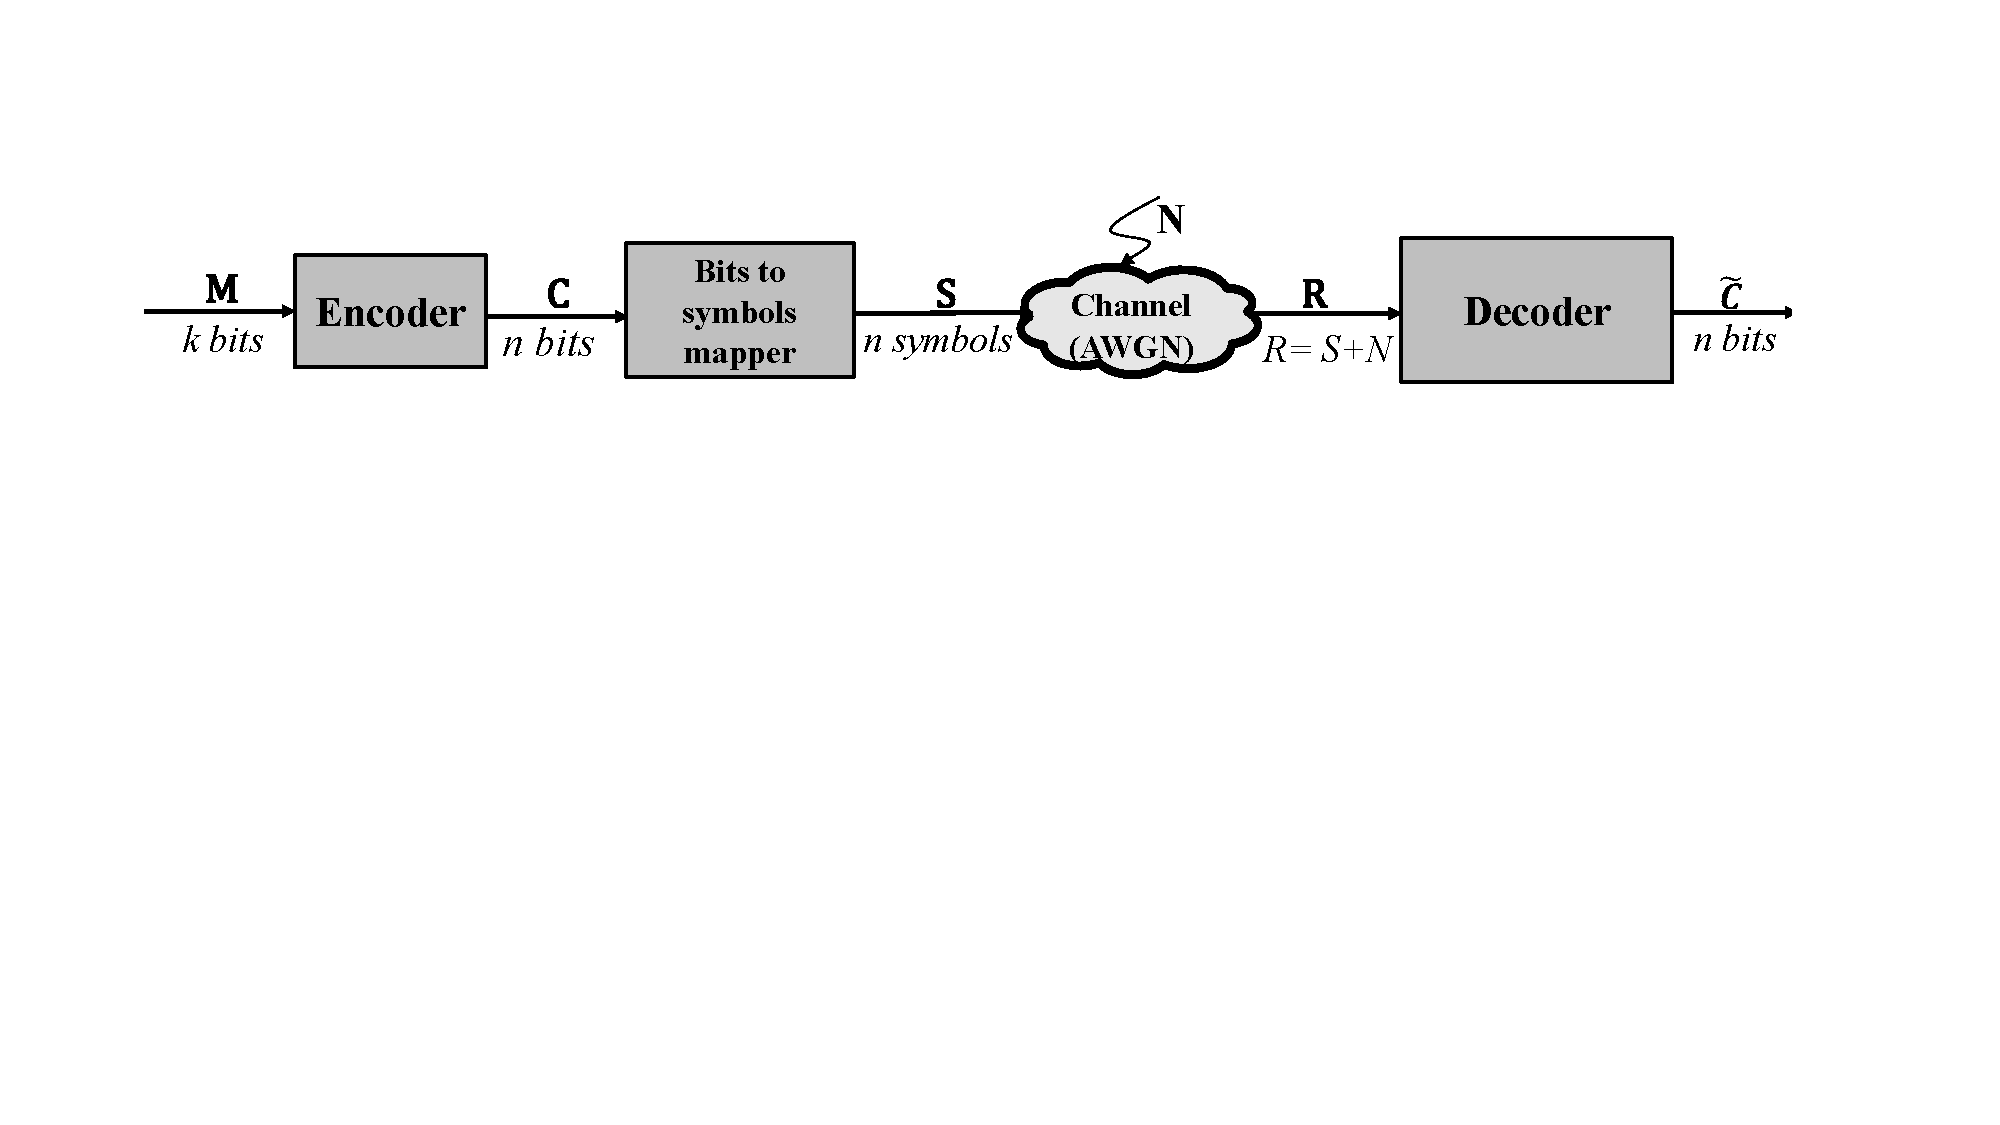
\includegraphics[width=0.50\textwidth]{FIGS/comunication_system.pdf}}
    \caption{Schematic diagram of communication system.}
    \label{fig:communication_digaram}
\end{figure}


%In this paper, we assumed a discrete communication system (Figure~\ref{fig:communication_digaram}),  where a $k$-bit binary message $M$ is  encoded into an $n$-bit code word ($C$) using a ($k$, $n$) LDPC code. This code word is modulated using the \emph{binary phase shift keying} (BPSK) modulation scheme, transmitted over a channel with additive white Gaussian noise (AWGN), and demodulated into received signal where $R_i=(1-2C_i)+\mathcal{N}(0, 1/SNR)$. 
%\todo{Professor please take a look at this paragraph }

In this paper, we assumed a discrete communication system (Fig.~\ref{fig:communication_digaram}), 
where a binary message $M$ with $k$-bit is encoded into an $n$-bit code word $C$ using a ($k$, $n$) LDPC  code. This code word is converted into an $n$-bit vector ($S_i = 1-2C_i$) of symbols representing a \emph{binary phase shift keying} (BPSK) constellation. This $n$-bit vector of symbols is transmitted over a channel with additive white Gaussian noise (AWGN). At the receiver end, we would receive a signal where $R_i=S_i+N(1/SNR)$, $N$ represents the channel's noise.


\subsection{Low Density Parity Check Codes}
LDPC codes are a class of linear block codes. The parity bits (redundant
information) are obtained using bitwise XOR operation on a selected number of
message bits. These codes are specified by a generator matrix $G_{k \times
n}$ or a parity check matrix $H_{m \times n}$, each of which can be obtained
from the other using the following relation $H\xor G^\top =0$. Here $m$ is
the number of parity bits, $n$ is the number of bits of the code word, and
$k$ is the number of bits in the message ($k=n-m$). The ratio of the length of
the message ($k$) to the size of the code word ($n$) is called the \emph{rate}: 
$r = k/n$. For example, the 5G standard uses 1/3 and 1/5 rate codes. 
The generator matrix is used for encoding a message ($M$) into a code 
word ($C$) using the following equation $C = G^\top\xor M$.
At the receiver side the decoded message is obtained from both the received
message ($R$) and the parity check matrix. The name ``low density" comes from the
sparse structure of the parity check matrix. 

\begin{figure}[htbp]
    \centering
    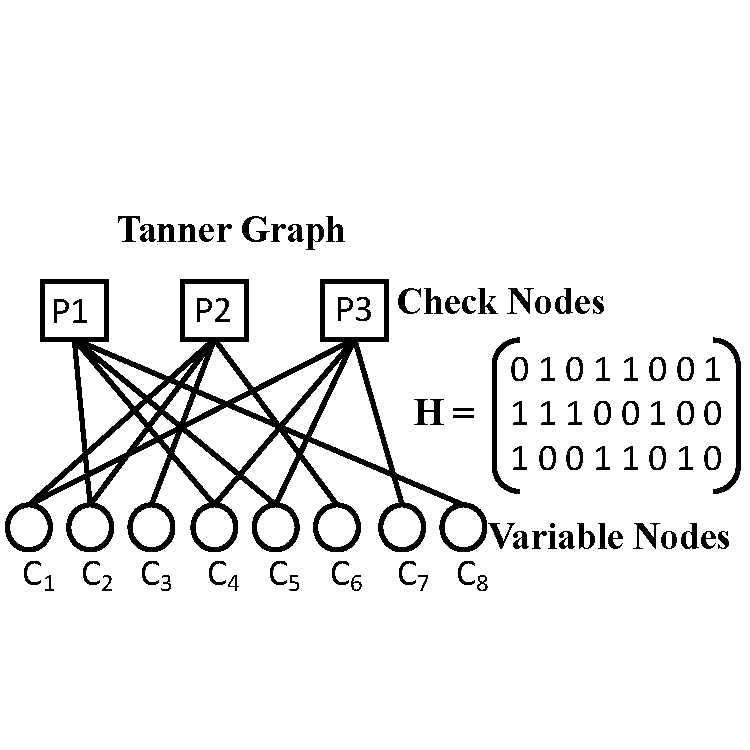
\includegraphics[width=0.38\textwidth]{FIGS/tanner_graph.pdf}
    \caption{Tanner graph with corresponding parity check matrix $H$.}
    \label{fig:tg}
\end{figure} 

LDPC codes can be represented graphically using Tanner graphs. These graphs are bipartite, meaning that the graph nodes are separated into two distinctive sets, and edges only connect nodes of two different types. The two types of nodes in a Tanner graph are variable and check nodes. Fig.~\ref{fig:tg} is an example of a Tanner graph that is constructed using parity check matrix $H$ shown above. It consists of $m$ check nodes (the number of parity bits) and $n$ variable nodes (the number of bits in an encoded message). Check node $P_i$ is connected to variable node $C_j$ if the element $h_{ij}$ of $H$ is a 1. These graphical structures are handy for analysis and decoding purposes.

%\note{I don't think the following commented paragraph is relevant.}

%There are many types of LDPC codes like regular, irregular, systematic, and nonsystematic. In regular code, the degree of rows and columns of parity check matrix are equal, i.e., the number of ones in every row is fixed. Similarly, the number of ones in every column is also fixed. In a systematic code, an encoded message is constructed with message bits followed by parity bits. The main advantage of systematic code is that the message can be directly obtained from the decoded word. The most commonly used LDPC codes are irregular systematic codes. These codes can also be constructed using a base graph as a template; hence they are called protographic~\cite{thorpe2003low}.

%\todo{fix citation above}
\begin{comment}
\subsection{Binary Phase shift Keying}
To efficiently transmit messages over communication channels, modulation schemes are employed. In this paper, we consider binary phase-shift keying (BPSK). This technique utilizes a single-frequency carrier signal and encodes digital data onto the signal by applying a phase shift. For a 0 in the data, no phase shift is applied; for a 1, the phase of the carrier signal is shifted by $180$ degrees. The data can then be recovered by the receiver by simply checking for the presence of this shift during each clock cycle by comparing it to a reference signal. If the carrier during that period has a phase shift present, the transmitted bit is decoded as 1; if not, the transmitted bit is decoded as 0.
 
Mathematically, encoding a message using BPSK modulation can be represented as follows. If $M$ is the message used for transmission, $S$ is the modulated signal, then $S = 1-2 \times M$. The received signal $R$ can be defined as $R= S+ n$, where $n$ is the noise added to the signal by the channel. 

\subsection{Decoding LDPC codes using Belief Propagation}

LDPC codes are often decoded using BP-style algorithms. The code word $\tilde{C}$ is decoded from the received message by calculating each bit's belief, or log-likelihood ratio (LLR), of being zero. 
The decoding process of LDPC code using BP is as follows: %uses tanner graph representation.
\begin{enumerate}
    \item First, the variable nodes in tanner graph are initialized using the intrinsic LLRs calculated using the received signal, and these values are broadcasted to the corresponding neighbor check nodes.
    \item Then an extrinsic LLR is calculated at each check node for each neighbor variable node based on the received LLRs from other neighbor variable nodes. Once the calculation is done, these extrinsic LLRs are again broadcasted back to each corresponding neighbor variable node.
    \item After receiving the extrinsic LLRs from the check nodes, LLRs are recalculated for each connected check node using both received extrinsic LLRs from other check nodes and the intrinsic LLR calculated from the signal.
    \item Once the calculation is done, it is broadcasted again to check nodes. This passing process is carried out until the maximum iteration count is attained or until the decoded code word can satisfy the parity check conditions.
\end{enumerate}
    This decoding methodology is also popularly known as a message-passing algorithm. There are many variants for this algorithm, like layered BP~\cite{hocevar2004reduced}, Offset Min-Sum, Normalized Min-sum~\cite{chen2005improved}, and more. These variants differ in the way they calculate the LLRs.   
    
\end{comment}

%\todo{is adjacent the same as neighboring? If so, use one to minimize confusion. Let's use "neighbor" which is simpler than "neighboring" without changing meaning.}

%\todo{make it sequential}
 \begin{comment}
 
 Let us assume the decode code word be $\tilde{C}$. Let the set of variable nodes that are connected to check node $c$ be denoted as $N(c)$, and the set of check nodes that are connected to variable node $v$ be denoted as M(v). Also $N(c)\backslash v$ and $M(v)\backslash c$ denote the set N(c) and M(v) excluding bit node v and check node c. The conventional iterative decoding process is based on the following steps:

\todo{Consistency in subscripting, and minimizing levels without ambiguity.}

%\note{A couple of ambiguities. $\tilde{c}$ is the decoded word, which means M+N bits long? But $c$ is a "node"? meaning it's not a word or related to word $\tilde{c}$, using deliberately the same letter implied some connection -- that one is a variation of the other.}

Step 1:

Each variable node $v$ is initialized using the intrinsic log-likelihood ratio  calculated by using following formula, 

\begin{equation}
    LLR_{v} = \log \frac{P(v=0/R)}{P(v=1/R)} = \frac{2R}{\sigma^2} 
\end{equation}

%\note{$0/r_i$ is still 0. Do you mean conditional probability given $r_i$}

where $\sigma$ represents the estimated variance of the Gaussian noise of the channel and $P(v=0/R)$ conditional probability of $v$ being zero, given $R$.

%\note{Do you mean estimated/assumed variance}

Step 2:

Once the LLR values are calculated at variable nodes, they are passed to the neighboring check nodes. Let $LLR_{v \rightarrow c}$ be the LLR received by the check node $c$ from variable node $v$.

At the check node $c$ for each neighboring variable node $v$, an extrinsic LLR ($LLR_{c \rightarrow v}$) is calculated  using equation~\ref{eq::llrc2v} and passed to that corresponding node.

\begin{equation}
%\begin{split}
    \label{eq::llrc2v}
    LLR_{c \rightarrow v} = 2 \times \arctanh\{   \\ \prod_{v_{i} \in N(c)\backslash v}  \frac{1+e^{-|LLR_{v_{i} \rightarrow c}|}}{1-e^{-|LLR_{v_{i} \rightarrow c } |}}\}
%    \end{split}
\end{equation}

Step 3:

After receiving the messages from the check nodes, the extrinsic messages to the neighboring check nodes are computed using equation ~\ref{eq::llrv2c} and passed to corresponding check nodes.

\begin{equation}
    \label{eq::llrv2c}
    LLR_{v \rightarrow c }  = \sum_{c_{i} \in M(v)\backslash c} LLR_{c{_i} \rightarrow v } + LLR_{v}
\end{equation}

The value of each bit of code word is decided at the variable node by calculating the final LLR by summing all LLRs received from the check nodes along with the intrinsic LLR. If the final LLR value is greater than zero, then the value of the bit is decided as zero; otherwise, 1. Step2 and Step3 are repeated until a maximum number of iterations are reached or if the decoded code word satisfies the constraint $H \xor c =\hat{0}$.

($LLR_{c \rightarrow v }$) calculated using equation~\ref{eq::llrc2v} is approximately equal to the minimum absolute value of the LLRs received from variable nodes. The sign of $LLR_{c \rightarrow v }$ is equal to the product of the sign of $LLR_{v \rightarrow c } $  all received at check node c. 

Based on this approximation, a variation of the Belief propagation called the Min-Sum algorithm was developed. The LLRs that need to be propagated to the neighbor variable node are calculated by replacing all the received LLRs with the minimum value, and the minimum value is replaced with the second minimum value. The product of the signs of received LLRs decides whether to flip the signs or not.
\end{comment}

%\todo{If this is a chapter, wouldn't this whole Ising model be described in detail somewhere earlier already? If so, this can be a very quick recall (e.g., keeping the equation), but not a repeat. Just point to the earlier chapter for detail.}
%\begin{comment}
    

\subsection{Ising Model}\label{sec:ising_mode}

The Ising model is used to describe the energy of a system of coupled
spins. The spins have one degree of freedom and take one of two values ($+1$,
$-1$). The energy of the system is a function of pair-wise coupling of the
spins ($J_{ij}$) and the interaction ($h_i$)
of some external field ($\mu$) with each
spin. The resulting energy is as follows:

\begin{equation}
\label{eqn:Ising_w_field}
% H = -\sum_{(i<j)} J_{ij}\sigma_i\sigma_j - \mu \sum_i h_i\sigma_i
E = -\sum_{\mathclap{(i<j)}} J_{ij}\sigma_i\sigma_j - \mu \sum_{\mathclap{i}} h_i\sigma_i
\end{equation}


A physical system with its energy defined by the formula naturally tends towards low-energy
states. It is as if nature tries to solve an optimization problem with
Eq.~\ref{eqn:Ising_w_field} as the objective function, which is not a trivial
task. Indeed, the cardinality of the state space grows exponentially with the
number of spins, and the optimization problem is NP-complete: it is easily
convertible to and from a generalized max-cut problem, which is part of the
original list of NP-complete problems~\cite{Karp1972}.

Thus if a physical system of spins somehow offers programmable coupling
parameters ($J_{ij}$ and $\mu h_i$ in Eq.~\ref{eqn:Ising_w_field}), they can
be used as a special purpose computer to solve\footnote{Throughout
the paper, by ``solving" an optimization problem we mean the
searching for a good solution rather than necessarily finding the global optimum, 
equivalent to reaching the ground state.} optimization problems that
can be expressed in the form of an Ising formula (Eq.~\ref{eqn:Ising_w_field}). In fact, all
problems in the Karp NP-complete set have their Ising formula
derived~\cite{lucas2014ising}. Also, if a problem already has a QUBO (quadratic
unconstrained binary optimization) formulation, mapping to Ising formula is as
easy as substituting bits for spins, \eg $\sigma_i = 2b_i-1$.

Because of the broad class of problems that can map to the Ising formula,
building nature-based computing systems that solve these problems has
attracted significant attention~\cite{kim2010quantum,berloff2017realizing,
barends2016digitized,yamaoka201520k,bunyk2014architectural,king2018observation,
bohm2019poor,hamerly2019towards,pierangeli2019large}.

\begin{comment}
Loosely speaking, an Ising machine's design goes through four
steps:
\begin{enumerate}

\item Identify the physical variable to represent a spin (be it a 
qubit~\cite{PhysRevB.82.024511}, the phase of an optical pulse~\cite{inagaki2016coherent}, 
or the polarity of a capacitor's voltage~\cite{afoakwa.hpca21}).

\item Identify the mechanism of coupling and how to program the coefficients.

\item Demonstrate the problem solving capability showing both the theory of its
operation (reveal the ``invisible hand" of nature) and satisfactory results
of practice.

\item Demonstrate superior machine metrics (solution time, energy consumption,
and construction costs).

\end{enumerate} 
\end{comment}

%It is important to note that different approaches may
%offer different fundamental tradeoffs and goes through varying gestation
%speeds. Thus it could be premature to evaluate a general approach based on
%observed instances of prototypes. Nevertheless, we provide a broad-brushed
%characterization, which can help researchers get a 
%basic sense of the landscape -- as long as the caveats are properly understood.
%\end{comment}


\begin{comment}
    

\subsection{Ising Machines}
\todo{Again, shouldn't this be present already elsewhere?}

We divide existing Ising Machines into three categories based on the technology used for their design: Quantum, Optical, and Electronic annealers. 

The latest Quantum Ising annealer manufactured by D-wave can support up to 2000 qubits~\cite{D-Wave}. The qubits are coupled to form a chimera graph. As a result of local coupling, the D-wave machine can only map up to 64 nodes all to all connected graph~\cite{hamerly2019experimental, hamerly2018scaling}. These annealers are also susceptible to noise, necessitating cryogenic operating condition that consumes much power (25KW for D-Wave 2000q)~\cite{dwave_stats}.

At the moment, the most powerful Ising machine is the Coherent Ising Machine (CIM)~\cite{inagaki2016cim, cim_yamamoto, McMahon614, 16bit_cim, ncomm_bohm2019}. It uses an optical parametric oscillator to generate and manipulate the signal to represent one spin. Unlike D-Wave, CIM nodes are all-to-all coupled. The machine has two components: an optical cavity built using kilometers of fibers, and an auxiliary computer to implement coupling between nodes. Every pulse's amplitude and phase in the optical cavity are detected, and its interaction with all other pulses is calculated using an auxiliary computer (FPGA). This computation is then used to modulate new pulses that are injected back into the optical cavity. Strictly speaking, the current implementation is a nature-simulation hybrid Ising machine. Thus, beyond the challenge of constructing the cavity, CIM  also requires a significant supporting structure that involves fast conversions between optical and electrical signals. 


 The operating principle of CIM can be viewed as a Kuramoto model~\cite{Takeda_2017},  so in theory, we can achieve a similar goal using other oscillators. This led to the design of an electronic Oscillator-based Ising Machines. These systems use LC tanks for spins and (programmable) resistors as coupling units. However, inductors are often a source of practical challenges for on-chip integration. They are area intensive and have undesirable parasitics with reduced quality and increased phase noise, which poses practical challenges in maintaining frequency uniformity and phase synchronicity between thousands of on-chip oscillators. 


Another electronic design with resistive coupling is the Bistable Resistively-coupled Ising Machine (BRIM)~\cite{afoakwa.hpca21}, in which the Ising spin is implemented as capacitor voltage controlled by a feedback circuit, making it bistable. Since it uses voltage (as opposed to phase) to represent spin, it enables a straightforward interface to implement additional architectural support for computational tasks. In BRIM, the polarity of the voltage across a capacitor represents the spin of the node and the coupling strength is inversely proportional to the resistance of the coupling resistors, i.e., $R_{ij}=\frac{R}{\abs{J_{ij}}}$, where $R$ is a scaling coefficient and the negative coupling is achieved by cross coupling the capacitors in neighboring nodes.
\end{comment}

\begin{comment}
\subsection{Existing LDPC decoders}
\todo{need to discuss about existing hardware LDPC decoders and existing Ising machines }

Most of the LDPC decoders in literature are designed by a hard-wiring a specific algorithm for a particular parity check matrix based on a chosen standard. ~\cite{?} discuss the design of LDPC decoder for 5g standard implementing offset Min-Sum Layered algorithm. The following design only supports the LDPC decoder for 5g base graph1 with an expansion factor of 384. ~\cite{?} discuss the design of the same 5g standard LDPC decoder implementing the same offset Min-sum algorithm but with support for all graphs possible in the standard. ~\cite{?} discuss pipelining the layered Min-sum algorithm for IEEE 802.e. standard to achieve high throughput.

Ising Machines have also been used for implementing decoders for LDPC codes. ~\cite{?} discuss how to convert LDPC codes into QUBO format and implement LDPC codes on D-wave. This implementation's main drawback is that it cannot fit an LDPC code of standards. This system's bit error rate (BER) is not as good as the Min-Sum algorithm's.
\end{comment}

\section {Co-designed Ising Machine Architecture}
\label{sec:arch}


%In this section, we discuss about the algorithm change to QUBO formulation of decoding of LDPC codes and it's formulation.
\subsection{Fundamentals of QUBO formulation of LDPC decoding}
\label{sec:QUBO_formulation}

The goal of LDPC decoding is to reproduce the original message $M$ with low bit error rates. 
This is modeled as a combinatorial optimization problem with two objectives: \begin{enumerate}
    \item The decoded output $\tilde{C}$ is a code word (satisfies parity check).
    \item It should be close to the received message $R$.
\end{enumerate}
If we use the BPSK modulation scheme, the objective function can be represented by Eq.~\ref{eq::obj}
where $\alpha$ adjusts the relative emphasis of the two objectives above.\footnote{Choosing $\alpha > \sum_{i=1}^{n} 4|R_i|$ is suggested~\cite{tawada2020new} to \emph{guarantee} the decode output is always a code word. In our observations, this choice results in poorer results than using empirically selected values.} \begin{equation}
\label{eq::obj}
\begin{split}
    F =  \sum_{i=0}^{n-1}(R_i - (1-2\tilde{C_i}))^2 + \alpha (H \xor \tilde{C})
\end{split}
\end{equation}

%\todo{shouldn't there be a factor before $H \xor \tilde{C}$ to determine how important satisfying parity check.}
\begin{comment}
\begin{equation}
\label{eq::obj}
\begin{split}
    F = \sum_{i=0}^{n-1}(R_i - (1-2\tilde{C_i}))^2 \\
   with\ constraint\ that\  H \xor \tilde{C} = \hat{0}
\end{split}
\end{equation}
\end{comment}

\subsubsection{Conversion to QUBO formulation}
Fundamentally, because of the presence of the XOR operation, Eq.~\ref{eq::obj}
is not a quadratic formula (\eg QUBO). Therefore it can not be directly mapped
to an Ising machine. There are multiple ways of converting the formulation into
a quadratic form, but here we only discuss one, which uses minimum auxiliary
spins~\cite{tawada2020new}. The general idea is straightforward: Satisfying
parity check means that $H\xor \tilde{C}$ is an all-zero vector. This in turns
means that the inner product of each row of $H$ with $\tilde{C}$ is an
even number. This can be represented as $H_j \cdot \tilde{C} = 2L_j$, where
$H_j$ is the $j$-th row of the parity check matrix ($H$), and $L_j$ is any integer.
This condition can be represented using the following objective function:
\begin{equation}
    F_s = \sum_{j=0}^{m-1}(\sum_{i=0}^{n-1} H_{j,i}\tilde{C}_i - 2L_j)^2.
\end{equation}
Since the integer $L_j$ is a free variable, it needs to be
to be represented by auxiliary variables $y_{j,k}\in \{0,1\}$. 
Given a fixed LDPC code, $L_j$ is
bounded: $0 \leq L_j \leq \lfloor \frac{|H_j|}{2} \rfloor $, where $|H_j|$
is the number of 1’s in $H_j$. 
This can be done in a number of ways with different tradeoffs. One approach is
\emph{unary} (or one-hot) encoding, another is \emph{binary} encoding as follows.
\begin{equation}\label{eq:unary_binary}
\begin{split}
    \text{Unary encoding:\;}&  L_j = \sum_{k=0}^{\lfloor \frac{|H_j|}{2} \rfloor} y_{j,k} \\
    \text{Binary encoding:\;}&
             L_j = \sum_{k=0}^{\lfloor \log_2 (\frac{|H_j|}{2})\rfloor} 2^k y_{j,k}
\end{split}
\end{equation}
Thus, the objective function can be written as: 
\begin{equation}
\label{eq::obj_ising}
    F = \sum_{i=0}^{n-1}\left(R_i - (1-2\tilde{C_i})\right)^2 + \alpha F_s,
\end{equation}
and after collecting terms,
$F$ can be written in the following format: 
\begin{equation}
F = x^\top Qx +c 
\end{equation}
where $x$ represents all binary variables including those of $\tilde{C}$ and the auxiliary variables $y_{j,k}$. The matrix $Q$ is mapped onto Ising machines to find $x$ as a solution for the decoding problem.

This conversion is necessary for a standard Ising machine. But it requires
extra spins. In fact, binary encoding (Eq.~\ref{eq:unary_binary}) almost
doubles the total number of spins required and unary encoding requires even
more. Keep in mind that the size of an Ising model's state space scales with
$2^n$ where $n$ is the number of spins. The added auxiliary spins not only
increase the hardware resource demand, but also has significant implications
on an Ising machine's ability to navigate through the solution space and thus
on the solution quality (see Sec.~\ref{sec:solution_quality}). To address the 
issue, we propose a new co-designed Ising machine architecture for LDPC decoding
without adding auxiliary spins. 

\subsection {Co-designed formulation and architecture}\label{secc:m_qubo} 

To see how an Ising machine architecture can be extended to support LDPC
decoding, we rewrite the decoding objective function (Eq.~\ref{eq::obj})
using spin representation to more easily map to the hardware implementation,
specifically $\Tilde{C_i}=0\rightarrow\sigma_i=1$, and 
$\tilde{C_i}=1\rightarrow \sigma_i=-1$.
With this rewrite, an XOR operation on a binary variable is converted into 
a multiplication operation of the corresponding spin variable as can be
seen in Table~\ref{tabel:truth_table}. 
Thus Eq.~\ref{eq::obj} can be written as follows:
\begin{equation}
\label{eq::mul_obj}
\begin{split}
    f = \sum_{i=0}^{n-1}(R_i - \sigma_i)^2  + \alpha \sum_{j=0}^{m-1}(1-\prod_{\mathclap{ H_{j,i}=1}} \sigma_i)/2.
\end{split}
\end{equation}
Since constants do not affect the objective function, we can remove them:
\begin{equation}
\label{eq::LDPC_ising}
\begin{split}
    f =  \sum_{i=0}^{n-1}-2R_i\sigma_i  -\frac{\alpha}{2}\sum_{j=0}^{m-1} 
    \sigma_i \sigma_{j\backslash i},\;\;
    where\ \sigma_{j\backslash i}\ =\ \prod_{\mathclap{H_{j,k}=1, k\neq i} } \sigma_k
\end{split}
%\sum_{\mathclap{\;\;\;H_{j,i}=1}} 
\end{equation}
%\todo{check the above formulation}

\begin{wraptable}{r}{1.5in}
%\vskip -20pt
\footnotesize
\centering
\caption{Truth table of bit XOR operation and spin multiplication  }
\setlength{\tabcolsep}{2pt}
\label{tabel:truth_table}
\begin{tabular}{|c|c|c|c|c|c|} 
\hline
$A$ &  $B$ &  $A \xor B$ & $\sigma_A$ & $\sigma_B$ & $\sigma_A.\sigma_B$ \\ 
\hline\hline
 0 &  0  & 0 & 1 & 1 & 1\\  
\hline
0  &  1 & 1 & 1 & -1 & -1\\   
\hline
1    & 0 & 1 & -1& 1& -1\\ 
\hline
1    & 1 & 0  & -1 & -1 & 1\\ 
\hline
\end{tabular}
\end{wraptable}

We can see that Eq.~\ref{eq::LDPC_ising} bears a significant resemblance to the Ising model 
(Eq.~\ref{eqn:Ising_w_field}) if we treat all $\sigma_{j\backslash i}$ as some (auxiliary) spins. 
Note that these spins are simply functions of regular spins.
We can thus design an \emph{augmented} Ising machine that uses extra logic to generate these
auxiliary spins which are coupled with regular spins. 

On the surface, the use of auxiliary spins would suffer the same drawbacks of using extra
spins discussed earlier (hardware cost and bloated state space). In reality, these spins  
are fundamentally different from the 
auxiliary spins resulted from Eq.~\ref{eq:unary_binary} in two important ways as follows
(quantitative results will be shown later in Sec.~\ref{sec:evaluations}).
\begin{enumerate}
    \item \textbf{Degree of freedom:} The auxiliary spins ($\sigma_{j\backslash i}$) do not have
    any additional degree of freedom. This means that fundamentally they do not increase the size
    of the state space. Consequently, they do not add to the difficulty of navigating the energy landscape.
    
    \item \textbf{Coupling complexity:} Another common drawback for using auxiliary spins is that the
    circuit complexity is dominated by couplers which scales quadratically with the number of spins. 
    Indeed, we can see in Eq.~\ref{eq::LDPC_ising} that there are many auxiliary spins needed. 
    Take only one checksum $j$ for instance and assume
    (for simplicity of argument) that it involves 10 regular spins $\sigma_{i1}$ to $\sigma_{i10}$. 
    Then each such spin requires its own auxiliary spins $\sigma_{j\backslash i1}$ to 
    $\sigma_{j\backslash i10}$. This repeats for every one of the $m$ checksums, easily leading
    to tens of thousands of spins for kilo-bit codes in theory. But in reality, as we will 
    discuss in detail later,
    there is significant regularity, structure, and sparsity in the coupling needed for
    real-world codes. As a result, a custom-designed Ising machine has very limited coupling
    complexity.
\end{enumerate}

%As suggested by Eq.~\ref{eq::LDPC_ising}, the couplings are only between a regular spin ($\sigma_i$) and specific auxiliary spins ($\sigma_{j\backslash i}$).




%Hence $P_{j\backslash i}$ in the following Equation~\ref{eq::LDPC_ising} can be calculated by XNORing the state of node $N_i$ with parity equation $P_j$. The parity equation can be evaluated by XNORing the nodes' states. For simplicity, in Equation~\ref{eq::LDPC_ising}, if we consider that the energy only depends upon satisfying the parity equations. The system implementing the following equation should flip the current states of nodes involved in an unsatisfied parity equation to achieve a code word that satisfies all the parity check equations. This behavior can be easily mimicked with a system of capacitors and XNOR gates.


%Figure~\ref{fig:circuit_digaram} shows the circuit implementation of Equation~\ref{eq::LDPC_ising} with a parity check matrix with only one parity equation. The voltage on capacitors represents the state of nodes. The parity equation $P$ is implemented by XNORing all the nodes involved \ie $V_1$ to $V_4$. $P_{\backslash i}$ at each node is calculated by XNORing the state of node $V_i$ with parity equation $P_j$.

%Suppose we consider $P$ being satisfied when it is high. In the Figure~\ref{fig:circuit_digaram}, when $P$ is high, the output of XNOR gates, connected to the capacitor of nodes representing $P_{\backslash i}$, is the same as that of the node's states. So when a parity equation P is satisfied, the states of nodes $V_1$ to $V_4$ are unchanged. When the parity equation ($P$) is low,  $P_{\backslash i}$ contradicts the node's states. So the output of XNOR gates will flip the states of nodes. Hence this circuit can find a code word that satisfies a parity equation. 

With this new formulation,
we now discuss the design of a complete system (illustrated in Fig.~\ref{fig:arch}), 
staring with \ding{172} the overall architecture centering on the coupling array 
architecture (Sec.~\ref{ssec:arch}), followed by \ding{173} circuit designs for spins, bias units, 
parity units, and coupling units (Sec.~\ref{ssec:circuit}).

\subsection{Architecture of the augmented Ising machine}
\label{ssec:arch}

In principle, any Ising machine can be adapted according to Eq.~\ref{eq::LDPC_ising}. In practice,
because the auxiliary spins are logical function of regular spins, we use BRIM~\cite{afoakwa.hpca21}
as the baseline. Its CMOS-compatible, voltage-based spins are more convenient for our purpose
than qubit- or phase-based machines~\cite{dwave-timing, wang2019oim}.

We first discuss the coupling array as it is by far the dominant component, generally containing $O(n^2)$ couplers
for $n$ spins. By default, there is a dense array of $n\times n$ \emph{programmable}
couplers to map the coupling coefficients $J_{ij}$ in Eq.~\ref{eqn:Ising_w_field}. A naive mapping
of Eq.~\ref{eq::LDPC_ising} for a $(k,n)$ parity code will require $n$ regular spins for the code
and up to $mn$ auxiliary spins for the parity checks. Fortunately, 
a number of customizations can be done to greatly simplify the overall architecture. 

\subsubsection{\bf Restricted and regular coupling}

To see the opportunity, let us use a concrete example and
assume a 6-spin, 2-checksum ($j=0,1$) system  
with the following quadratic coupling: \begin{equation}
\color{lightgray}\sum_{j=0}^{m-1}(1-\prod_{\mathclap{ H_{j,i}=1}} \sigma_i) \rightarrow \color{black}
\underbrace{(1-\sigma_1\sigma_3\sigma_5)}_{\text{checksum } j=0}+\underbrace{(1-\sigma_2\sigma_4\sigma_6)}_{j=1}
\label{eq:chksum_ex}
\end{equation}
Nominally we need 6 auxiliary spins ($\sigma_{0\backslash 1}$,
$\sigma_{0\backslash 3}$,
$\sigma_{0\backslash 5}$,
$\sigma_{1\backslash 2}$,
$\sigma_{1\backslash 4}$,
$\sigma_{1\backslash 6}$), making a total of 12 spins (and about 144 couplers).
But the coupling is actually restricted. Only an auxiliary spin is coupled to
a regular spin, and only in one direction -- the output of the auxiliary spin determines the current inflow to a regular
spin and can thus potentially change it.

Furthermore, within one checksum, the multiple auxiliary spins (\eg $\sigma_{0\backslash 1}$,
$\sigma_{0\backslash 3}$, $\sigma_{0\backslash 5}$) are ultimately reflection of the 
same parity checksum (the XOR of bits 1, 3, and 5). 
Another important regularity is that the coupling strengths are all the same. Combined
together, this means that a single auxiliary spin is needed per checksum and each 
coupler can be now implemented via a simplified control circuit, which we discuss
in Sec.~\ref{ssec:circuit}). Finally, the coupler is only needed when a spin is part
of the checksum.

Combining these factors, in our running example, we end up requiring only 2 auxiliary spins
and 6 total couplers. In fact, there are additional opportunities because  most
standards use proto-graph-based codes which have additional structures 
(see Box 1) that we can exploit as follows.



\begin{figure}[t]
\begin{boxedminipage}{\columnwidth}
\textbf{\small Box 1. LDPC matrix structure for 5G }
\vskip 8pt
\parskip 0.8ex
%\scriptsize
%\footnotesize
\small
In this paper, we discuss LDPC for the latest standard called 5G new radio (NR)~\cite{tr20175g} by the 3rd-generation partnership project (3GPP) for wireless enhanced-mobile broadband (eMBB) communication. 

The 5G standard uses two base-graph (BG) matrices: BG1 and BG2, which are used to construct a parity check matrix. Fig.~\ref{fig:5g-nr} shows the structure of BG1. The blue dots in Fig.~\ref{fig:5g-nr} show nonzero elements of the matrix. It has 46 rows and 68 columns (BG2 matrix is 42$\times$52). Rows in the base graphs describe parity check equations. By default, BG1 generates an LDPC code with a rate equal to $1/3$, and BG2 generates an LDPC code with a rate equal to $1/5$. 

\begin{wrapfigure}{r}{1.8in}
    \vskip -5pt
    \hskip -5pt
    {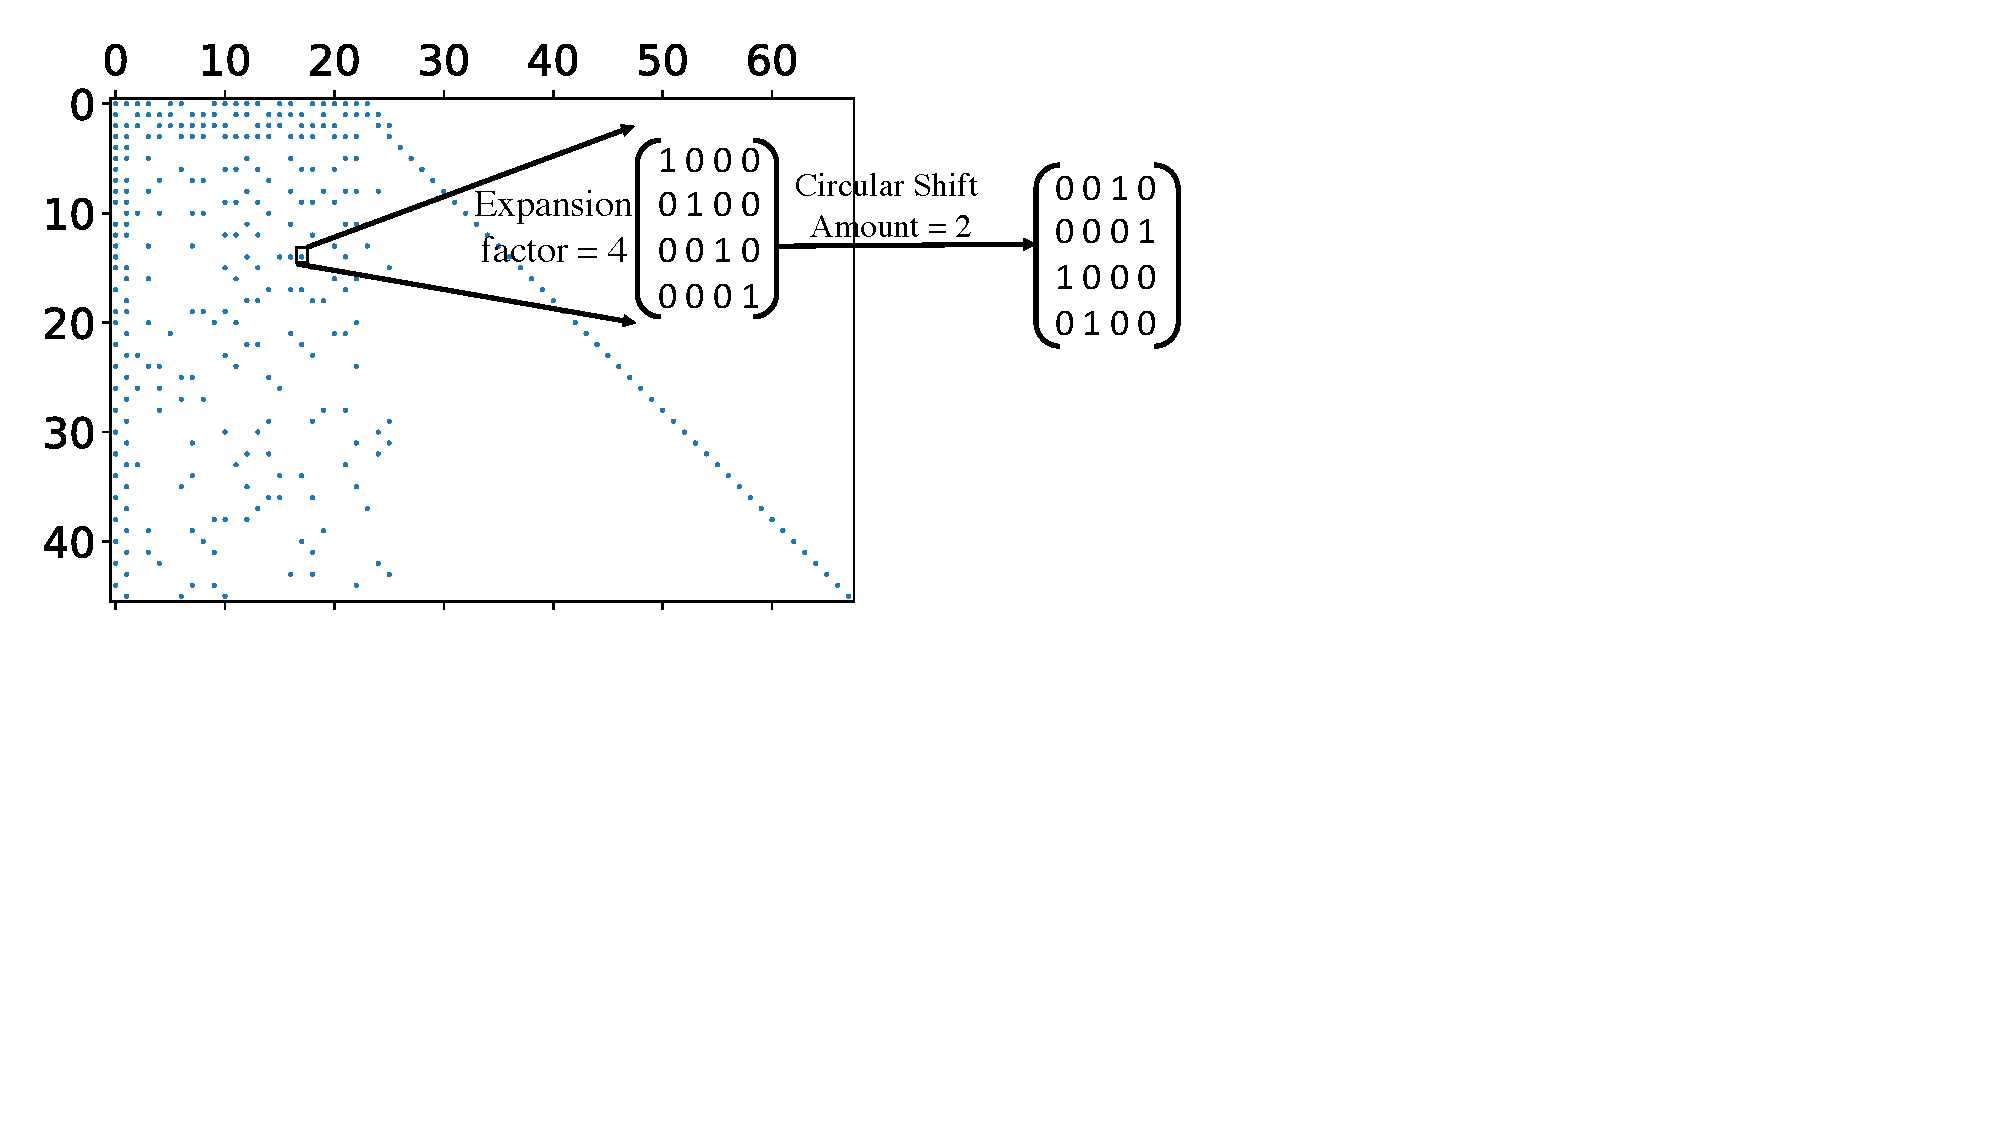
\includegraphics[width=1.9in]{FIGS/circular_shift.pdf}}
    \caption{Structure of 5G-NR standard base graph 1. Each blue dot represents a nonzero element which will be replaced by a circular identity matrix based on the expansion factor as shown.}
    \label{fig:5g-nr}
\end{wrapfigure}

Once the base graph is chosen, each zero entry is replaced with a $Z \times Z$ all-zero matrix. Each nonzero entry is replaced with a $Z \times Z $ circularly shifted identity matrix. $Z$ is called an expansion factor. The amount of circular shift depends on the value of the nonzero element. The values of the nonzero elements range from 0 to $Z-1$. If the value is 0, replace the element with the $Z \times Z$ identity matrix; otherwise, circularly shift the identity matrix based on the value. Fig.~\ref{fig:5g-nr} shows an example with an expansion factor of 4 and a circular shift amount of 2. The 5G-NR standard allows different discrete expansion factors ranging from 2 to 384. For further details, please refer to \cite{bae2019overview}.
\end{boxedminipage}
\end{figure}

\begin{figure}[htp]
    \centerline{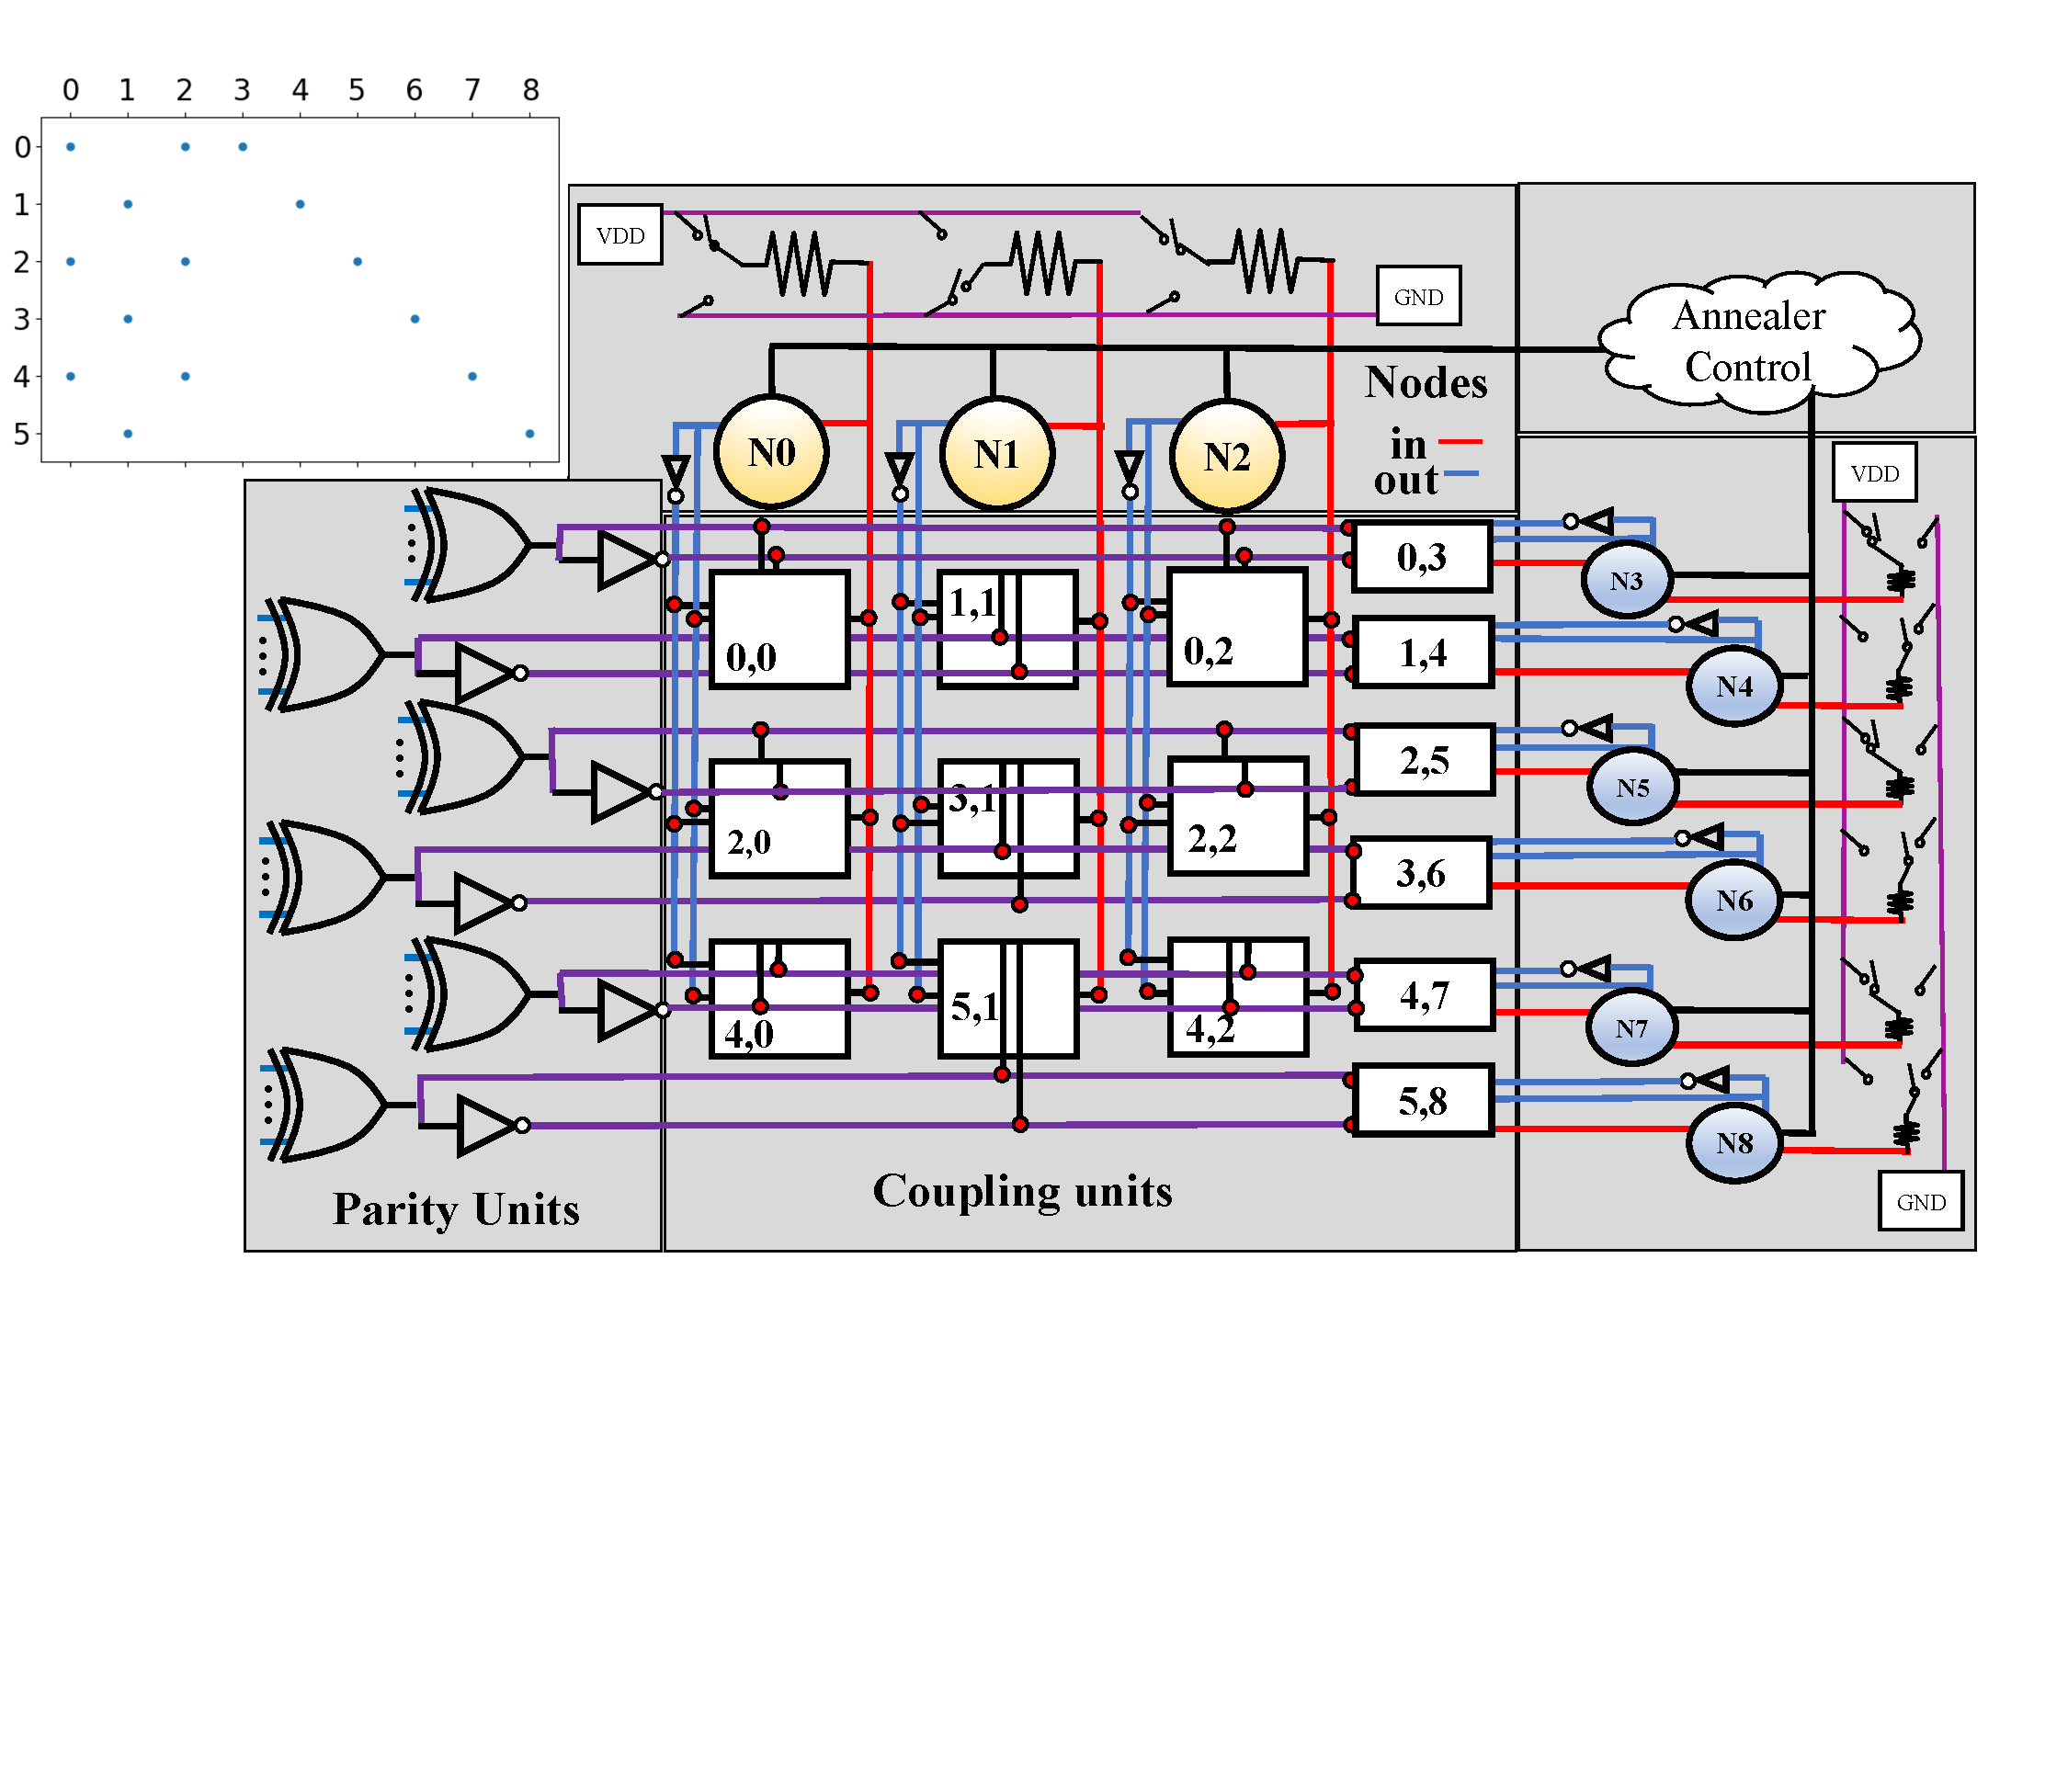
\includegraphics[width=0.50\textwidth]{FIGS/ldpc_arch_new_new1.pdf}}
    \caption{Illustration of our Ising machine-based LDPC decoder using a specific portion 
    (shown in top left) of the parity check matrix.} \label{fig:arch}
    %\todo{need to add pseudo matrix }
\end{figure}

\subsubsection{\bf Structure of the matrix}
As the name low-density suggests, the matrix is rather sparse, reducing the number of couplers
needed. A particular property of the 5G base matrix is that a large portion of the code bits
are only involved in a single parity check (so-called extension checks). In other words, many
columns (representing bits) have only one non-zero element. This portion is organized as a
diagonal submatrix and can be seen in Fig.~\ref{fig:5g-nr}. Because these spins have only one
coupler, their couplers can be easily incorporated into their node design. Overall, the coupling
array can be organized as a 2-d grid with auxiliary spins (parity checks) as one dimension
regular spins as another, with the checksum bit having single parities forming a special column.
The structure is shown in Fig.~\ref{fig:arch}.

To recap, with this architecture, the number of couplers equals the number of 1s in the
parity check matrix and is thus a constant (given a matrix), not affected by the number of
auxiliary spins we added. The auxiliary spins are generated from the XOR of all bits involved
in a parity check and thus have no degrees of freedom on their own. The state space of the
dynamical system is only a function of the number of regular spins.



\subsection{Circuit design}
\label{ssec:circuit}

\subsubsection{\bf Nodes}

In our baseline Ising machine~\cite{afoakwa.hpca21}, the spins are represented 
by voltage polarities on capacitors. %which are terminated to a \emph{virtual} ground (at half $V_{dd}$).
When representing $\sigma_i=+1$, corresponding to bit $\tilde{C_i}=0$,
the capacitor has a positive voltage.
Conversely, for $\sigma_i=-1$, its voltage is negative.

In the circuit implementation of the proposed Ising machine,
a spin is stored on a capacitor, and a node maintains the spin 
and interfaces with other circuits with its input/output circuit.
Fig.~\ref{fig:QuBRIM_node} shows an initial circuit design of a node. 
Besides the spin capacitor, it consists of three core functional blocks: 
a current conveyor, a one-bit quantizer, and a pair of spin-fix (SF) switches.
This node circuit takes an input current at $IN$, and generates an output voltage at $OUT$. 
The $OUT$ port of a node carries quantized voltage signals to both parity units and coupling units. 
The $IN$ port receives currents from coupling units. 
The node output can also be stored synchronously as a bit by an additional D flip-flop (DFF) when necessary.

%\begin{figure}[htp]
%\centering
%\includegraphics[width=0.30\textwidth]{LDPC codes/FIGS/qubrim_node.pdf}
%\caption{Circuit implementation of Node of LDPC decoder.} \label{fig:QuBRIM_node}
%\end{figure}

The current conveyor is constructed as a class-AB current mirror~\cite{kawahito1996cmos} %\cite{see Team QuiCC referenc}, 
which is designed for high slew rate and large input dynamic range. 
$M_5$-$M_8$ convey the input current from port $IN$ to node $Z$, 
hence charging/discharging the capacitor. 
The two current sources $I_{bias}$ set the bias condition for $M_1$-$M_4$, 
and hence the operating-point voltage at $Y$ is equal to that at $X$. 
By biasing node $X$ to $V_X=1/2(V_{DD}-V_{SS})$, 
$V_Y$ is effectively biased to the same voltage. 
The input impedance (at port $IN$) of this circuit is low,
allowing port $IN$ to operate as a current input.

\begin{wrapfigure}{r}{1.7in}
     {\includegraphics[width=1.7in]{FIGS/qubrim_node.pdf}}
     \caption{Circuit implementation of Node of LDPC decoder.}
     \label{fig:QuBRIM_node}
\end{wrapfigure}

The capacitor's voltage at node $Z$ represents the spin state: 
$V_Z<V_X$ for $\sigma_i=-1$, and $V_Z>V_X$ for $\sigma_i=+1$.
Note that this voltage $V_Z$ is an \emph{analog} signal, and needs to be quantized 
before it is used as an input for the XNOR gates in the parity and coupling units. 
Since our system operates in continuous-time, 
this quantizer can be simply constructed with inverters in series. 
In Fig.~\ref{fig:QuBRIM_node}, $M_{9-12}$ function as both a quantizer and super-buffer.

In order to configure the system's initial spins, 
%before the machine's states are allowed to evolve in seeking an energy minimum
two switches ($S_{1,2}$) are connected to node $Z$ to set/reset it to $V_{DD}$ or $V_{SS}$. 
We can also use these two switches to perform spin-fix perturbations, 
which allow the machine to escape local minima in search of the optimal solution. 
$SF_i^+$ and $SF_i^-$ are two non-overlapping control signals generated by the \emph{Annealer Control} unit.

\subsubsection{\bf Auxiliary spins and couplings}



For the auxiliary spins represent parity checks, 
let us consider the concrete case of checksum $j=0$ in Eq.~\ref{eq:chksum_ex}
($\tilde{C_1} \xor \tilde{C_3}\xor \tilde{C_5}$)
(the spin-based representation is $(1-\sigma_1\sigma_3\sigma_5)/2$). 
The physical meaning of the coupling is quite straightforward: 
when $\tilde{C_1}\xor \tilde{C_3}\xor \tilde{C_5}=0$,
each node will receive one unit of current keeping the node in the same polarity.
Conversely, when $\tilde{C_1}\xor \tilde{C_3}\xor \tilde{C_5}=1$, each node will
receive one unit of current trying to change the polarity of the node. 
We achieve this by generating the checksum ($\tilde{C_1}\xor\tilde{C_3}\xor \tilde{C_5}$)
to select for each spin whether to couple to its positive or negative edge of its own
node. An alternative view is that the selector acts as an additional XOR gate to
``back out" its own node. Thus, for node 1, the coupling comes from 
$\tilde{C_1} \xor \tilde{C_3}\xor \tilde{C_5}\xor\tilde{C_1}=\tilde{C_3}\xor \tilde{C_5}$.
%\begin{wrapfigure}{r}{3in}
%    {
\includegraphics[width=3in]{LDPC codes/FIGS/circuit_diagram_ldpc_pass.pdf}}
%    \caption{Logical implementation of proposed LDPC decoder.}
%    \todo{show the new pass gate based coupling controlled by a single auxiliary spin. Also use the
%    same orientation as the matrix}
%    \label{fig:circuit_digaram}
%\end{warpfigure}

\begin{figure}[htp]
\centerline{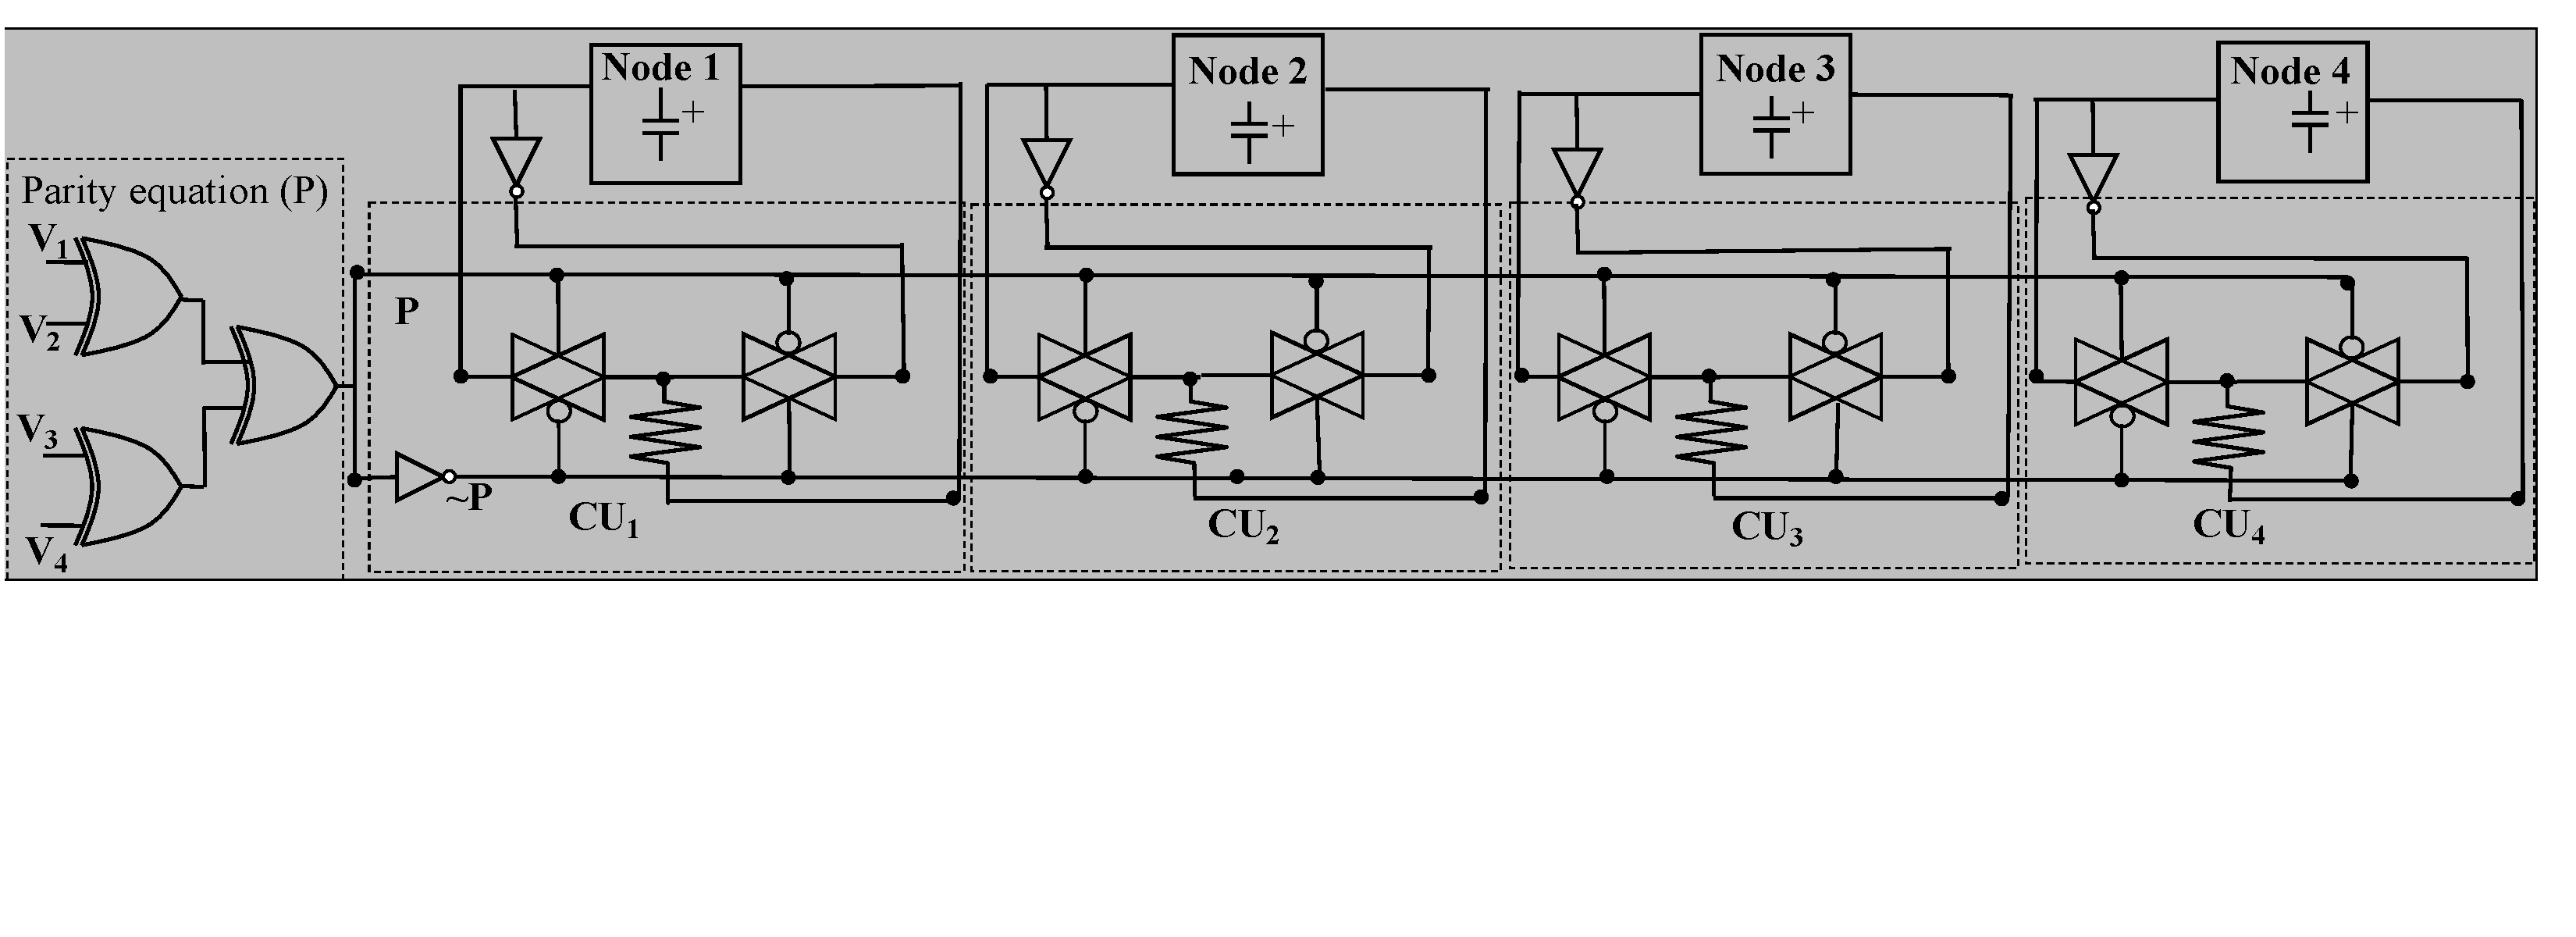
\includegraphics[width=0.5\textwidth]{FIGS/circuit_diagram_ldpc_pass.pdf}}
    \caption{Circuit implementation of parity check and its coupling to spins.} \label{fig:circuit_digaram}
\end{figure}

    %\todo{show the new pass gate based coupling controlled by a single auxiliary spin. Also use the same orientation as the matrix}
%We apply an additional optimization to reduce circuitry. This is best explained through an example. Let us assume row $j$ of $H$ has 4 non-zero elements, which we will simply refer to as Nodes 1 to 4. As the discussion above shows, each node will need an auxiliary spin that is the result of XOR of the other three nodes, \eg Node 2 will couple with the XOR of Nodes 1, 3, 4. This can be easily done by generating the XOR of all four nodes and then ``back out", say, Node 1 (by XOR'ing with it again) just before coupling with Node 1's capacitor.  Fig.~\ref{fig:circuit_digaram} shows the circuit.


%\subsubsection{\bf Parity, Coupling, and Bias Units}   Parity units represent the parity check equations or rows of a parity check matrix. As our design hardwires a particular parity check matrix, parity units are a binary tree of XNOR gates. These units are used to evaluate $P_j$ in the Equation~\ref{eq::LDPC_ising}. For the base graph 1 of the 5G standard, the maximum number of nodes involved in a parity check equation is 19; hence the maximum height of the binary tree will be five stages. As shown in the Figure~\ref{fig:arch} the output of each parity unit is fed into the columns of coupling units if a node ($N_i$) is involved in a parity check equation ($P_j$), the coupling unit ($CU_{i,j}$) is used for coupling the parity equation with the node. The coupling unit consists of an XNOR gate and a resistor. The output of the XNOR gate is connected to the $IN$ terminal of the node through a resistor. It determines the value of $P_{j \backslash i}$ and passes it to node $N_i$. The value of the resistor varies according to the $\alpha$ value. The bias represents the linear term in the Equation~\ref{eq::LDPC_ising}. It is implemented as a resistor connected to either VDD or GND, depending upon the sign of $R$. The absolute value of $R$ determines the value of the resistor.

\subsubsection{\bf Bias}
The linear terms ($-2R_i\sigma_i$ in Eq.~\ref{eq::LDPC_ising}) helps to 
constrain the decoded output closer to the received message, and is implemented by a 
bias current at each node proportional to the received value $R_i$. 
More specifically, according to Eq.~\ref{eq::LDPC_ising}, the bias current for
node $i$ needs to be $\frac{4R_i}{\alpha}$ time that of the coupling current from
the parity check. The sign of $R_i$ determines the polarity of the bias current. 

Putting everything together, 
Eq.~\ref{eqn:rim_node_simplifed} describes the circuit behavior.
We can see that if we use voltage $v_i$ (relative to virtual ground) 
as an approximation for spin $\sigma_i$ in Eq.~\ref{eq::LDPC_ising}, 
Eq.~\ref{eqn:rim_node_simplifed} is proportional to the gradient.
\begin{equation}\label{eqn:rim_node_simplifed}
\begin{split}
%    \dv{v_i}{t} = \frac{1}{C}(I_{in}) =  \frac{1}{C} \left[ \sum_{\mathclap{j}} J_{ij}*(P_{j\backslash i}) + {J_b}_i*({v_b}_i) \right]
    \dv{v_i}{t} = \frac{1}{C}(I_{in}) =  \frac{1}{C} \left[ \sum_{\mathclap{j}} J_{ij}*(P_{j\backslash i}) + {J_b}_i*({v_b}_i) \right] \\
    \dv{v_i}{t} = \frac{J}{C}(I_{in}) =  \frac{J}{C} \left[ \frac{4R_i}{\alpha}*{v_b}_i  + 
    \sum_{\mathclap{H_{j,i}=1}} \sigma_{j\backslash i} \right]
\end{split}
\end{equation}

 %As shown in Fig ~\ref{fig:PU} an XNOR gate (X1) with inputs $V_i+$ and $P_j^{in}$ are used to determine function \ding{172}. The output of the gate X1 is connected to $V_i-$ via a programmable coupling resistor ($T_1$) which acts as a switch. The programmable coupling resistor is implemented using a transistor whose charge on gate capacitance determines if the switch is on or off. According to parity equation $P_j$, if node $V_i$ is involved, then the switch $T_1$ would be turned on; otherwise, off. \ding{173} function is implemented using another XNOR gate (X2). As shown in Fig ~\ref{fig:PU} the inputs of XNOR (X2) gate are $P_j^{out}$ and $V_i+$.  $P_j^{out}$ represents the value of the parity equation ($P_j$) determined by the previous nodes in the column. If node $V_i$ is involved in the equation, then the node's current state should be XNORed with $P_j^{out}$ to determine the final value. If it is not involved in the equation, we should pass the value on to other nodes. To implement this, we used two switches $T_2$ and $T_3$ operating conversely. If node $V_i$ is involved then $T_2$ is turned on and $T_3$ is off; otherwise $T_3$ is turned on and $T_2$ is left off. These coupling resistors are programmed using a row selector and a column selector, which will be discussed in the next section. After determining the final value of $P_j$, it is passed as input to the parity units to calculate $P_j\backslash i$. The nodes c1, c2, and c3 in Figure~\ref{fig:BRIM_arch} represent the connection of wires between the $P_j^{out}$ and $P_j^{in}$. In this way, we have changed the architecture, nodes, and coupling unit structure of BRIM to directly map the LDPC decoding problem to the system. The rest of the unit's functionality is the same as BRIM, but we discuss it here also.
%Figure~\ref{fig:arch} shows architecture design of our LDPC decoder for a  base graph with 3 rows and 4 columns and for an expansion factor of 4. It has three main architectural components, \ding{172}  Node units blocks (N1 to Nn), \ding{173} parity units Block, \ding{174} check nodes units block (CNB1 to CNB3). The shaded regions represent zero elements in the base graph. Each block is replaced with an array of units based on the expansion factor as shown in figure. These units are hardwired based on the parity check matrix. The rows in~\ref{fig:arch} represent columns of the base graph and vice versa.
%Row $i$ are used for calculating $\sum_j P_{j\backslash i}$ of a node $i$ by summing the output currents from parity units of that row. Column $j$ is used to evaluate the parity equation "$P_j$." 

\begin{comment}    

\subsubsection{\bf Nodes}

We slightly modified bistable nodes $v_i$ of BRIM to implement biasing. In Fig.~\ref{fig:node_and_iv} we show a more detailed illustration of one node. A ZIV diode is used as the feedback circuit to stabilize the voltages at the desired levels (\eg $\pm V_{dd}$). The figure shows the IV curve of the ZIV diode. When capacitor voltages are in between $-V_{dd}$ and $V_{dd}$, the diode acts as an active element charging its voltage closer to $\pm V_{dd}$. Conversely, for voltages outside the range, the ZIV diode acts essentially as a linear resistor to discharge the capacitor. 

Each node is supplied with two pairs of switches to set the capacitor voltage to a known spin state. It is helpful for specific initialization or to change the system state as described in the  "Annealing Control "(Sec.~\ref{ssec:anneal_control}). Finally, the spin of the node can be read 
out by a digital latch (\eg a D flip-flop) connected to the ZIV diode's 
$V+$ terminal. It converts the spin to a bit (1 or 0). The pins labeled $V+$, and $V-$ are used to connect to the parity units' inputs and outputs. The bias determined by the received message is applied as a voltage through resistors (B+, B-) as shown in figure~\ref{fig:node_and_iv}. The value of resistance depends upon the value and sign of the received message.

\begin{figure}[htp]\centering
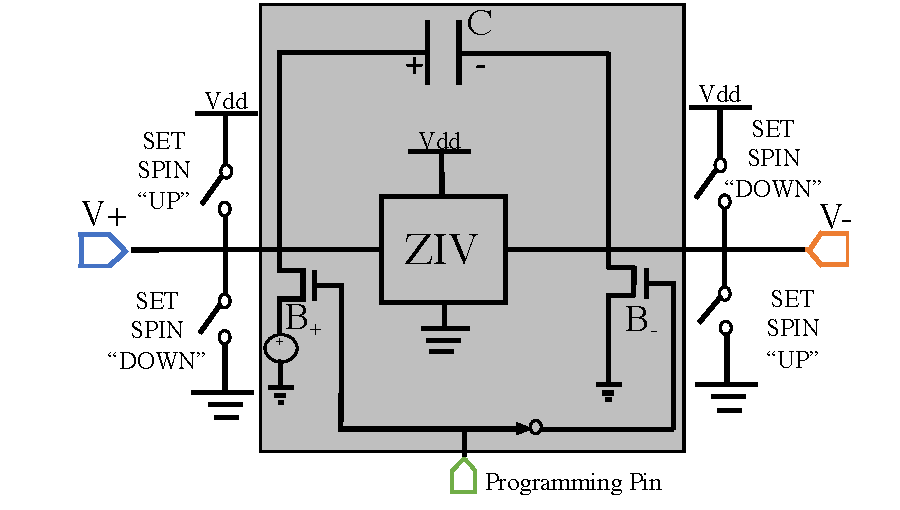
\includegraphics[width=0.28\textwidth]{FIGS/variable_node.pdf}
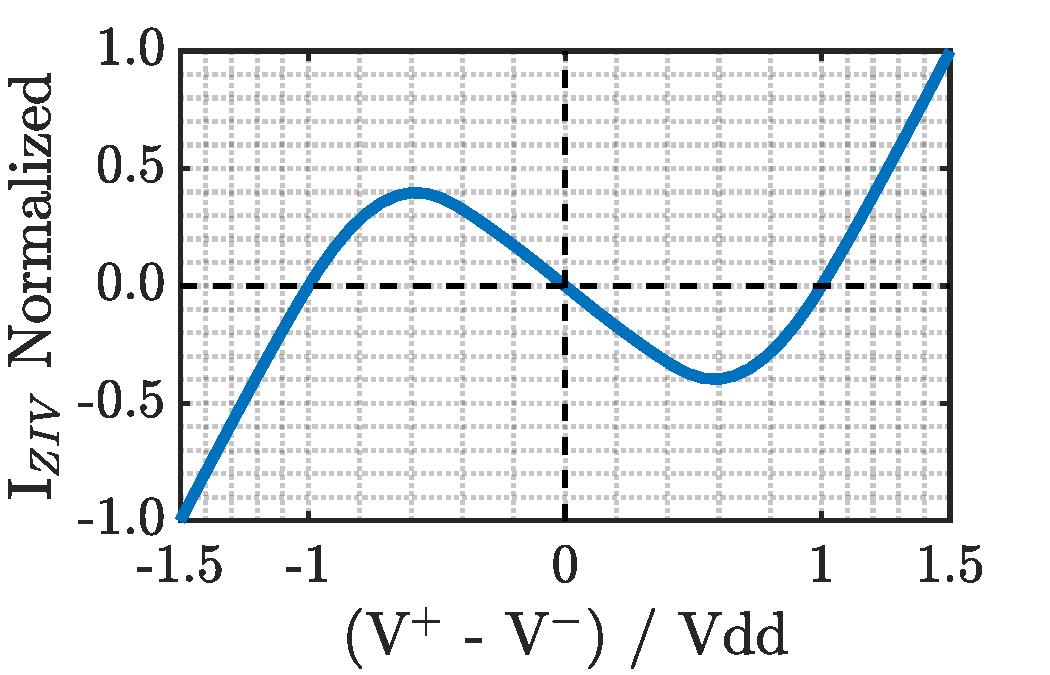
\includegraphics[width=0.20\textwidth]{ziv_curve.pdf}
\caption{Simplified schematic of one BRIM node (left) and ZIV diode's IV 
characteristic (right). \label{fig:node_and_iv}}
\end{figure}

\subsubsection{\bf Parity Unit}

The parity unit ($PU_{ij}$) represents the coupling unit in BRIM. Here, it is used for coupling node $V_i$ to parity equation $P_j$ and vice versa. It has the following functionalities \ding{172} to determine value $P_{j \backslash i}$ and pass it to node $V_i$ ,\ding{173} to evaluate the parity equation $p_j$ if node $V_i$ is connected to parity equation $P_j$, otherwise just pass the previous value of $P_j$ value to other nodes in same column.

 As shown in Fig ~\ref{fig:PU} an XNOR gate (X1) with inputs $V_i+$ and $P_j^{in}$ are used to determine function \ding{172}. The output of the gate X1 is connected to $V_i-$ via a programmable coupling resistor ($T_1$) which acts as a switch. The programmable coupling resistor is implemented using a transistor whose charge on gate capacitance determines if the switch is on or off. According to parity equation $P_j$, if node $V_i$ is involved, then the switch $T_1$ would be turned on; otherwise, off. \ding{173} function is implemented using another XNOR gate (X2). As shown in Fig ~\ref{fig:PU} the inputs of XNOR (X2) gate are $P_j^{out}$ and $V_i+$.  $P_j^{out}$ represents the value of the parity equation ($P_j$) determined by the previous nodes in the column. If node $V_i$ is involved in the equation, then the node's current state should be XNORed with $P_j^{out}$ to determine the final value. If it is not involved in the equation, we should pass the value on to other nodes. To implement this, we used two switches $T_2$ and $T_3$ operating conversely. If node $V_i$ is involved then $T_2$ is turned on and $T_3$ is off; otherwise $T_3$ is turned on and $T_2$ is left off. These coupling resistors are programmed using a row selector and a column selector, which will be discussed in the next section. After determining the final value of $P_j$, it is passed as input to the parity units to calculate $P_j\backslash i$. The nodes c1, c2, and c3 in Figure~\ref{fig:BRIM_arch} represent the connection of wires between the $P_j^{out}$ and $P_j^{in}$. In this way, we have changed the architecture, nodes, and coupling unit structure of BRIM to directly map the LDPC decoding problem to the system. The rest of the unit's functionality is the same as BRIM, but we discuss it here also.
 
\begin{figure}[htp]
    \centerline{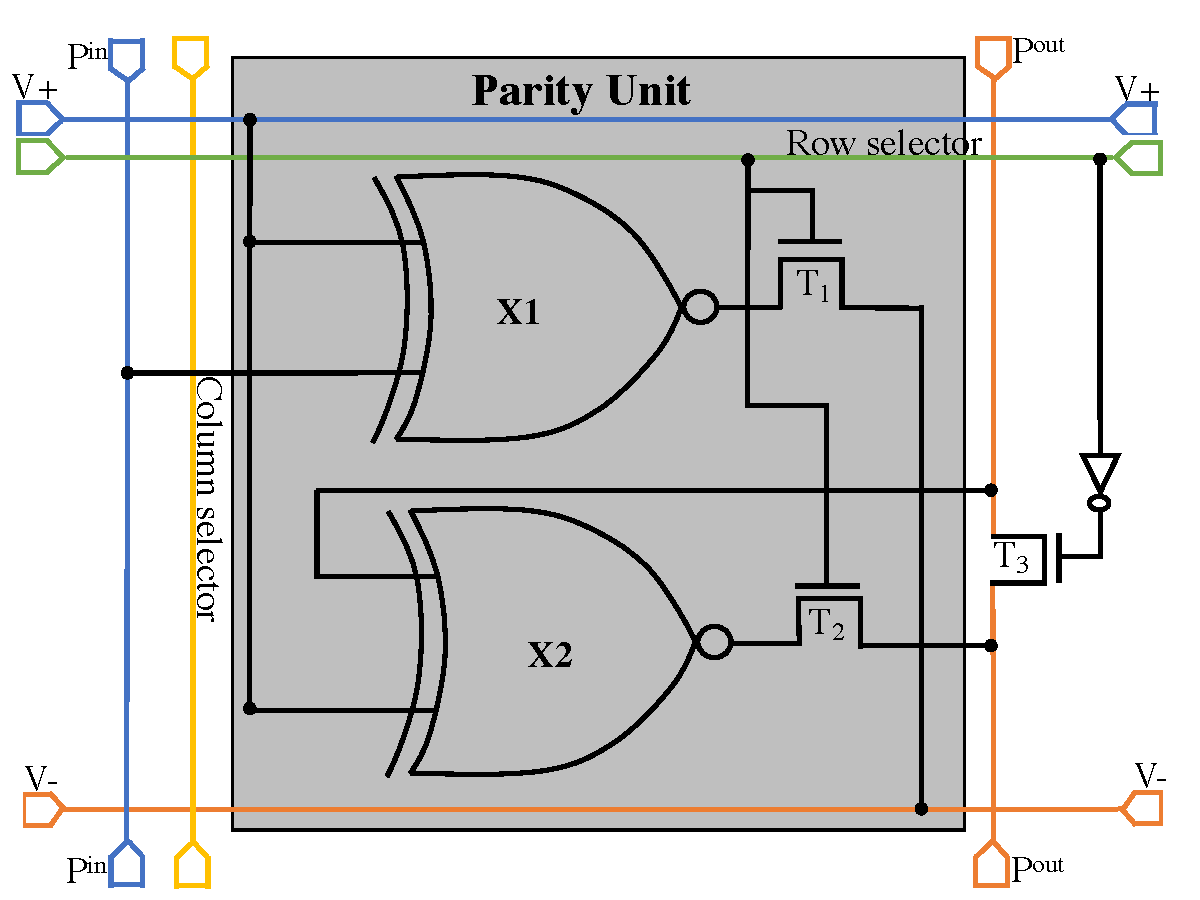
\includegraphics[width=0.5\textwidth]{FIGS/parity_unit_ldpc.pdf}}
    \caption{Schematic of parity unit. Color schemes are matched to system-level block diagram in Fig ~\ref{fig:arch} }
    \label{fig:PU}
\end{figure}

\end{comment}
%If the sign of the message is positive, switch B+ is turned on, and B- is turned off, and vice versa. These switches are programmed using the programming pin.
%\end{comment}

\begin{comment}
    

\subsubsection{\bf Programming units}
Both the initial nodal values and the coupling resistances in parity units are programmable.
Programming of a resistor is achieved through a transistor with adjustable 
gate voltage.
% The details of the circuit design are discussed in Appendix~\ref{ ssec:circuit}. 
To the right of the parity unit array in 
Fig.~\ref{fig:arch} is the programming array. This array consists of 
digital memory for storing the weights which drive an array of digital-to-analog 
converters (DACs).

A small amount of such DACs are sufficient to program all the parity units in a time-interleaved fashion per column. In such configuration, 
we need corresponding column selectors and pull-down logic as shown below 
the coupling units in Fig.~\ref{fig:arch}.

\subsubsection{\bf Annealing control}\label{ssec:anneal_control}

As our system is primarily an optimizer, it can get stuck in local minima. To avoid this, two commonly used mechanisms for annealers were adopted and incorporated to allow the system to escape local optima. First, the coupling strength is globally increased over time. In this way, at the very beginning, the machine is only weakly coupled, rendering the energy landscape relatively flat. It helps the system explore the landscape in a coarse granularity. We choose an exponential annealing schedule because (a) it is a common practice, and (b) it can be conveniently achieved by discharging an appropriately-sized capacitor as the global annealing scheduler. The voltage from this capacitor is then used to control the variable gain buffer in each node to achieve the change in coupling strength.

Second, we adopt a similar strategy as that used in simulated annealing. In Simulated annealing, the spins are flipped based on a probability decided by the differences in the energy. Doing the same thing in hardware is a complex process. To simplify the process, we use a "spin fix"; we randomly choose a node and briefly clip it to one of the supply rails. The nodal spin either maintains its current state or swaps to the opposite state. The probability/frequency of spin fixes is determined based on temperature. The temperature follows the same exponential annealing schedule discussed above. In other words, the frequency of spin fixes decays exponentially over time.
\end{comment}

%\subsection{Theoretical analysis}
%\todo{needs to be changed}
%We can theoretically define the evolution of above described LDPC decoder using equation~\ref{eqn:rim_node_simplifed}. It shows how the voltage of a capacitor representing each node change over time. $J_{ij}$ represents the effective conductance of the coupling with the parity equations. $B_i$ represents the bias current representing the bias term in the equation~\ref{eq::LDPC_ising}. %and  $g_{\!_{ZIV}}(v_{i})$ represents the current due to $ZIV$ diode.
%\begin{equation}\label{eqn:rim_node_simplifed}
%\begin{split}
%    \dv{v_i}{t} = \frac{1}{C}(I_{in} - I_{ZIV}) =  \frac{1}{C} \left[ \sum_{\mathclap{j}} J_{ij} P_{j\backslash i} + B_i  \right]
%\end{split}
%\end{equation}
%With this equation, we can provide the same Lyapunov stability analysis as shown in the following paper~\cite{afoakwa.hpca21} to prove our ability for optimum-seeking

\begin{comment}

\subsection{Architecture of hybrid LDPC decoder}
\label{ssec:arch}

We now discuss the architectural changes made to BRIM to implement an LDPC decoder. The system is illustrated in Fig.~\ref{fig:BRIM_arch} and consists of: 
\ding{172} bistable nodes (V1 to V4) and their digital interface (DFF 1-4); 
\ding{173} parity units connecting the nodes ($PU_{ij}$); \ding{174} 
programming units to configure parity units (including: memory, multiplexers,
digital-to-analog converters, and the column control systems); and \ding{175} annealing control. The rows (i) represent the variable nodes, and the columns (j) represent check nodes in a Tanner graph. Row $i$ is used for calculating $\sum_j P_{j\backslash i}$ of a node $i$ by summing the output currents from parity units of that row. Column $j$  is used to evaluate the parity equation "$P_j$." We discuss each unit in turn as follows:

\begin{figure}[htp]
    \centerline{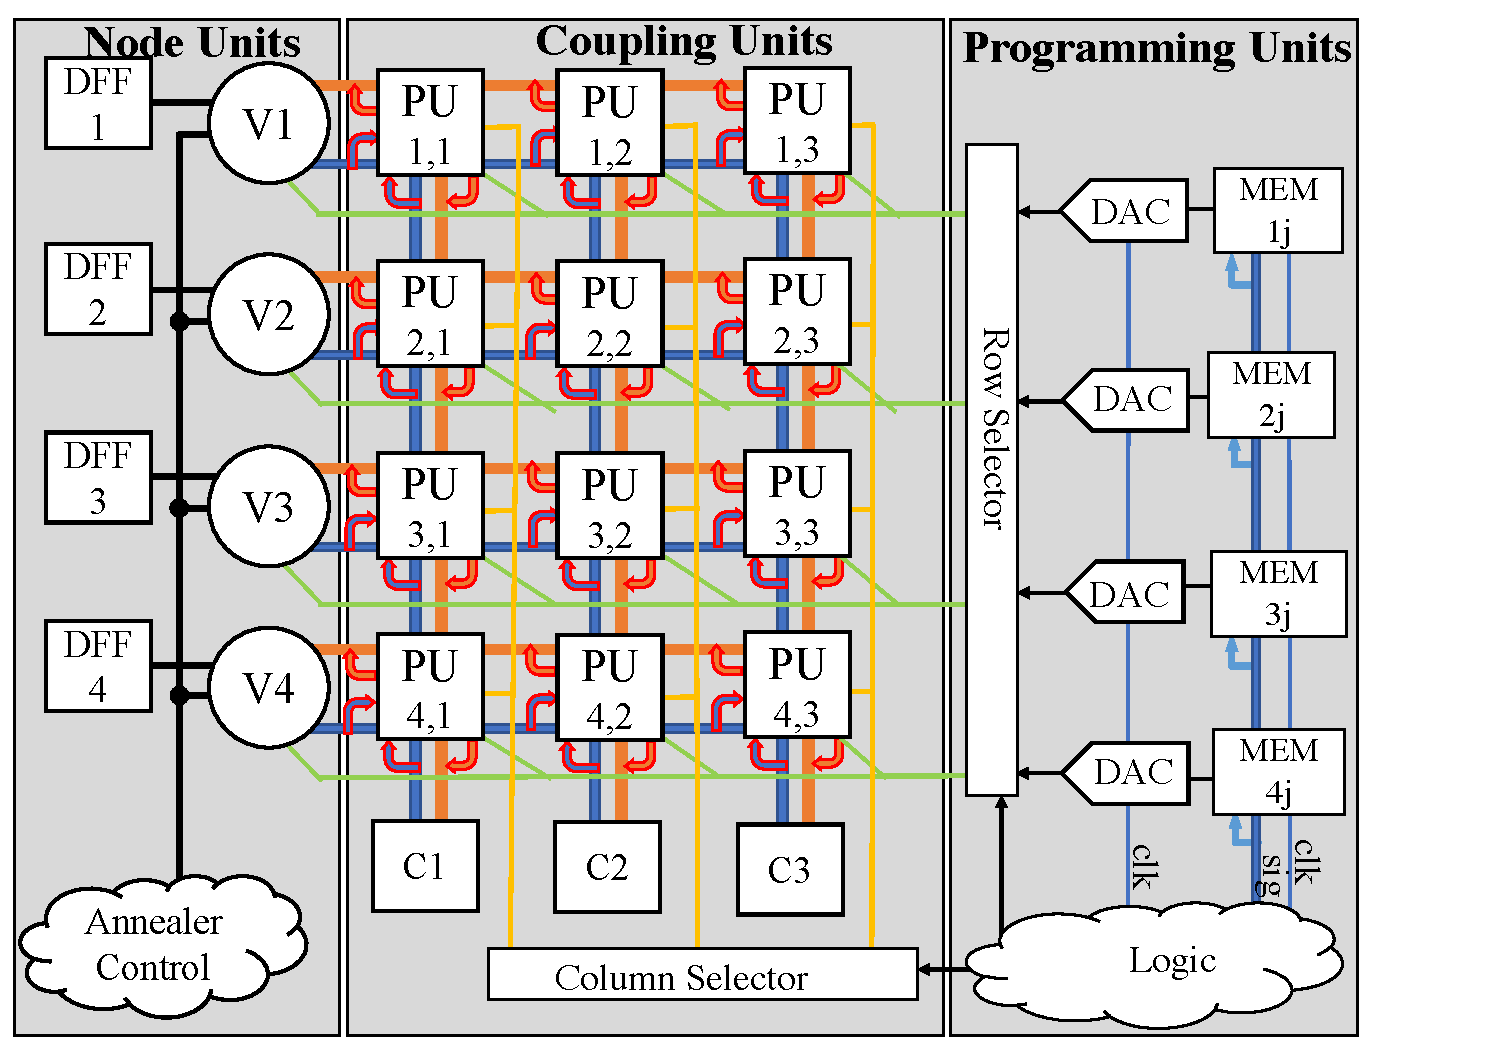
\includegraphics[width=0.45\textwidth]{FIGS/ldpc_new_arch.pdf}}
    \caption{Block diagram of BRIM based LDPC decoder's system components. Nodes are $N_i$ and parity units $PU_{i,j}$. The multi-colored interconnecting links are wires}
    \label{fig:BRIM_arch}
\end{figure}

\subsubsection{\bf Nodes}

We slightly modified bistable nodes $v_i$ of BRIM to implement biasing. In Fig.~\ref{fig:node_and_iv} we show a more detailed illustration of one node. A ZIV diode is used as the feedback circuit to stabilize the voltages at the desired levels (\eg $\pm V_{dd}$). The figure shows the IV curve of the ZIV diode. When capacitor voltages are in between $-V_{dd}$ and $V_{dd}$, the diode acts as an active element charging its voltage closer to $\pm V_{dd}$. Conversely, for voltages outside the range, the ZIV diode acts essentially as a linear resistor to discharge the capacitor. 

Each node is supplied with two pairs of switches to set the capacitor voltage to a known spin state. It is helpful for specific initialization or to change the system state as described in the  "Annealing Control "(Sec.~\ref{ssec:anneal_control}). Finally, the spin of the node can be read 
out by a digital latch (\eg a D flip-flop) connected to the ZIV diode's 
$V+$ terminal. It converts the spin to a bit (1 or 0). The pins labeled $V+$, and $V-$ are used to connect to the parity units' inputs and outputs. The bias determined by the received message is applied as a voltage through resistors (B+, B-) as shown in figure~\ref{fig:node_and_iv}. The value of resistance depends upon the value and sign of the received message.

%If the sign of the message is positive, switch B+ is turned on, and B- is turned off, and vice versa. These switches are programmed using the programming pin.

\begin{figure}[htp]\centering
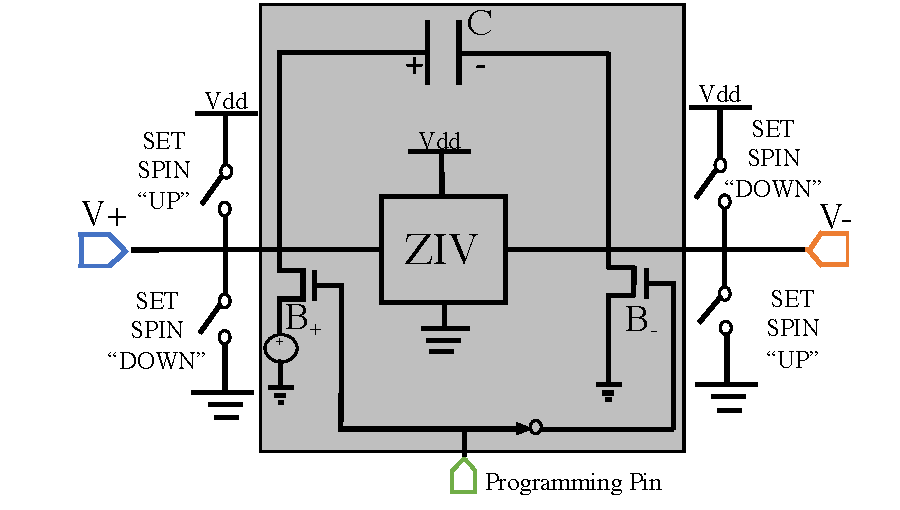
\includegraphics[width=0.28\textwidth]{FIGS/variable_node.pdf}
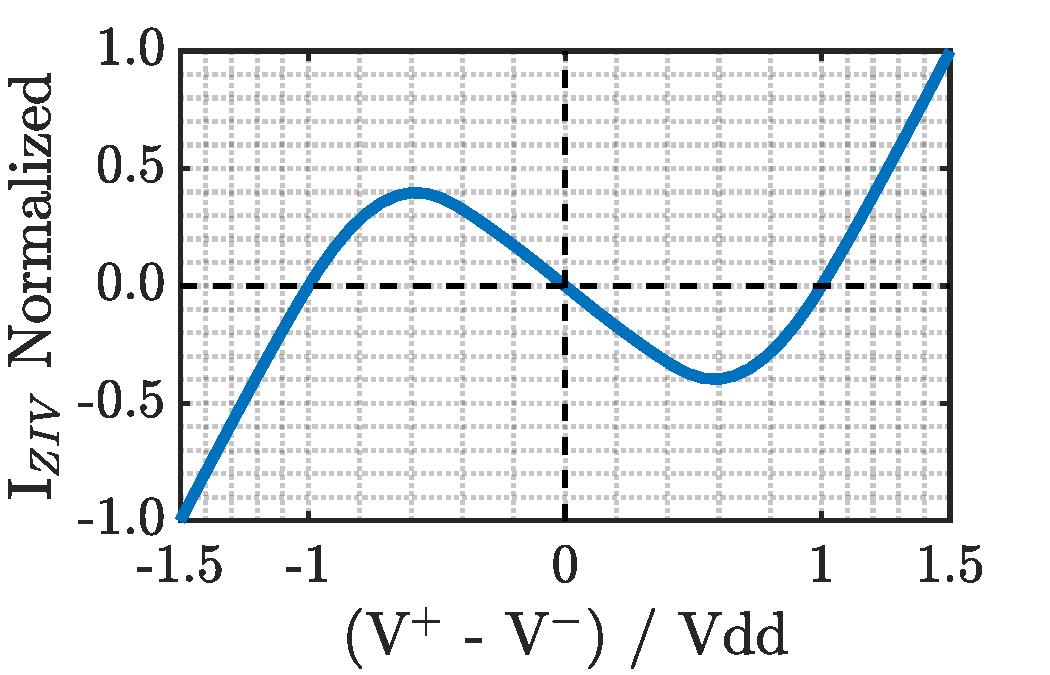
\includegraphics[width=0.20\textwidth]{ziv_curve.pdf}
\caption{Simplified schematic of one BRIM node (left) and ZIV diode's IV 
characteristic (right). \label{fig:node_and_iv}}
\end{figure}

\subsubsection{\bf Parity Unit}

The parity unit ($PU_{ij}$) represents the coupling unit in BRIM. Here, it is used for coupling node $V_i$ to parity equation $P_j$ and vice versa. It has the following functionalities \ding{172} to determine value $P_{j \backslash i}$ and pass it to node $V_i$ ,\ding{173} to evaluate the parity equation $p_j$ if node $V_i$ is connected to parity equation $P_j$, otherwise just pass the previous value of $P_j$ value to other nodes in same column.

 As shown in Fig ~\ref{fig:PU} an XNOR gate (X1) with inputs $V_i+$ and $P_j^{in}$ are used to determine function \ding{172}. The output of the gate X1 is connected to $V_i-$ via a programmable coupling resistor ($T_1$) which acts as a switch. The programmable coupling resistor is implemented using a transistor whose charge on gate capacitance determines if the switch is on or off. According to parity equation $P_j$, if node $V_i$ is involved, then the switch $T_1$ would be turned on; otherwise, off. \ding{173} function is implemented using another XNOR gate (X2). As shown in Fig ~\ref{fig:PU} the inputs of XNOR (X2) gate are $P_j^{out}$ and $V_i+$.  $P_j^{out}$ represents the value of the parity equation ($P_j$) determined by the previous nodes in the column. If node $V_i$ is involved in the equation, then the node's current state should be XNORed with $P_j^{out}$ to determine the final value. If it is not involved in the equation, we should pass the value on to other nodes. To implement this, we used two switches $T_2$ and $T_3$ operating conversely. If node $V_i$ is involved then $T_2$ is turned on and $T_3$ is off; otherwise $T_3$ is turned on and $T_2$ is left off. These coupling resistors are programmed using a row selector and a column selector, which will be discussed in the next section. After determining the final value of $P_j$, it is passed as input to the parity units to calculate $P_j\backslash i$. The nodes c1, c2, and c3 in Figure~\ref{fig:BRIM_arch} represent the connection of wires between the $P_j^{out}$ and $P_j^{in}$. In this way, we have changed the architecture, nodes, and coupling unit structure of BRIM to directly map the LDPC decoding problem to the system. The rest of the unit's functionality is the same as BRIM, but we discuss it here also.
 
\begin{figure}[htp]
    \centerline{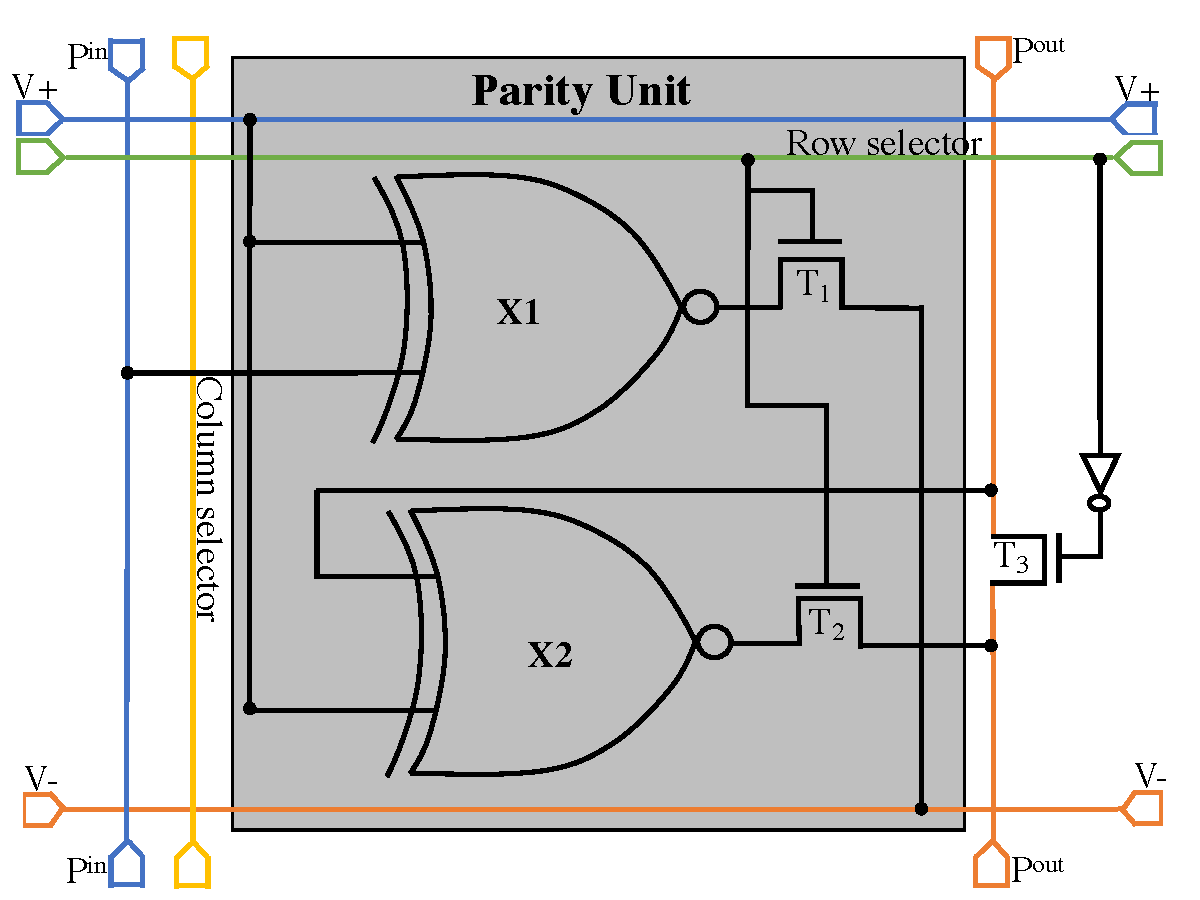
\includegraphics[width=0.5\textwidth]{FIGS/parity_unit_ldpc.pdf}}
    \caption{Schematic of parity unit. Color schemes are matched to system-level block diagram in Fig ~\ref{fig:BRIM_arch} }
    \label{fig:PU}
\end{figure}

\subsubsection{\bf Programming units}
Both the initial nodal values and the coupling resistances in parity units are programmable.
Programming of a resistor is achieved through a transistor with adjustable 
gate voltage.
% The details of the circuit design are discussed in Appendix~\ref{ ssec:circuit}. 
To the right of the parity unit array in 
Fig.~\ref{fig:BRIM_arch} is the programming array. This array consists of 
digital memory for storing the weights which drive an array of digital-to-analog 
converters (DACs).

A small amount of such DACs are sufficient to program all the parity units in a time-interleaved fashion per column. In such configuration, 
we need corresponding column selectors and pull-down logic as shown below 
the coupling units in Fig.~\ref{fig:BRIM_arch}.

\subsubsection{\bf Annealing control}\label{ssec:anneal_control}

As our system is primarily an optimizer, it can get stuck in local minima. To avoid this, two commonly used mechanisms for annealers were adopted and incorporated to allow the system to escape local optima. First, the coupling strength is globally increased over time. In this way, at the very beginning, the machine is only weakly coupled, rendering the energy landscape relatively flat. It helps the system explore the landscape in a coarse granularity. We choose an exponential annealing schedule because (a) it is a common practice, and (b) it can be conveniently achieved by discharging an appropriately-sized capacitor as the global annealing scheduler. The voltage from this capacitor is then used to control the variable gain buffer in each node to achieve the change in coupling strength.

Second, we adopt a similar strategy as that used in simulated annealing. In Simulated annealing, the spins are flipped based on a probability decided by the differences in the energy. Doing the same thing in hardware is a complex process. To simplify the process, we use a "spin fix"; we randomly choose a node and briefly clip it to one of the supply rails. The nodal spin either maintains its current state or swaps to the opposite state. The probability/frequency of spin fixes is determined based on temperature. The temperature follows the same exponential annealing schedule discussed above. In other words, the frequency of spin fixes decays exponentially over time.



\subsection{Theoretical analysis}

We can theoretically define the evolution of above described LDPC decoder using equation~\ref{eqn:rim_node_simplifed}. It shows how the voltage of a capacitor representing each node change over time. $J_{ij}$ represents the effective conductance of the coupling with the parity equations. $B_i$ represents the bias current representing the bias term in the equation~\ref{eq::LDPC_ising} and  $g_{\!_{ZIV}}(v_{i})$ represents the current due to $ZIV$ diode.

\begin{equation}\label{eqn:rim_node_simplifed}
\begin{split}
    \dv{v_i}{t} = \frac{1}{C}(I_{in} - I_{ZIV}) =  \frac{1}{C} \left[ \sum_{\mathclap{j}} J_{ij} P_{j\backslash i} + B_i - g_{\!_{ZIV}}(v_{i}) \right]
\end{split}
\end{equation}

With this equation, we can provide the same Lyapunov stability analysis as shown in the following paper~\cite{afoakwa.hpca21} to prove our ability for optimum-seeking.
\end{comment}

\begin{comment}
\todo{The commented section was not checked in editing -Andrew}

\subsection{Theoretical analysis} \label{ssec:theory}

\todo{Need to be modified}
We present same  Lyapunov stability analysis
of our LDPC decoder to show its ability for optimum-seeking as shown in the following paper~\cite{afoakwa.hpca21}.
Fig.~\ref{fig:brim} shows a simplified node $i$ in LDPC decoder where other nodes are 
coupled into $i$ from the right.
Writing the current equation, we get Eq.~\ref{eqn:rim_node_simplifed}, where $J_{ij}$ is the 
effective conductance of the coupling taking into account the polarity of
the coupling:
\begin{equation}\label{eqn:rim_node_simplifed}
\begin{split}
    \dv{v_i}{t} = \frac{1}{C}(I_{in} - I_{ZIV}) =  \frac{1}{C} \left[ \sum_{\mathclap{j}} J_{ij} P_{j\backslash i} - g_{\!_{ZIV}}(v_{i}) \right]
\end{split}
\end{equation}

LDPC decoder is a continuous time system where the state is summarized by
$v(t)=[v_1(t), v_2(t), ...\,, v_N(t)]^T$. (For brevity, in the following, $v_i(t)$
will be abbreviated as $v_i$.) Recall that in Lyapunov analysis, if a function
$H(v)$ can be found such that $\dv{H(v)}{t} = 0$ at point $v^e$
and $\dv{H(v)}{t} < 0$ in the region around $v^e$, then $v^e$ is the
equilibrium point~\cite{nonlinear_system_analysis}. In our case, this point is the solution to the equation set
$\dv{v_i}{t} = 0;\ i=1..N$.
\donotshow{\footnote{For those unfamiliar with the analysis, here is a roughly
explanation: if the condition $\dv{H(v)}{t} \leq 0$ is satisfied in a region
$v \in W$, that means once the system enters region $W$ at time $t_0$,
function $H(v(t))$ can only decrease or maintain its value (because its time
derivative is non-positive), thus a future state then clearly $H(v)$ can not
increase for a dynamical system can be identified, the system can be shown to
be stable at points where the function reaches minimum.}}
In other words, once the system enters a region, it will inevitably evolve
towards lowering $H(v)$ (because its time derivative is negative) until
it reaches the equilibrium point $v^e$.

To ensure $\dv{H(v)}{t}$ is non-positive, we can construct
it to be in a negative square form. This can be achieved 
by imposing the following construction rule.
\begin{equation}
\label{eqn:rule}
\pdv{H(v)}{v_i}=-\alpha\dv{v_i}{t}; \ \alpha>0
\end{equation} 

Following the chain rule, it is not difficult to see that:
\begin{equation}
\label{eqn:H_partials}
\dv{H(v)}{t} =\sum_{\mathclap{i}}\left(\pdv{H(v)}{v_i}\dv{v_i}{t} \right)
=-\alpha\sum_{\mathclap{i}}\left(\dv{v_i}{t}\right)^2
\end{equation}

One choice of a Lyapunov function satisfying the conditions in Eq.
\ref{eqn:rule} is shown in Eq.~\ref{eqn:Lyap_RIM}, where $G(v_i)$ is obtained
from $g_{\!_{ZIV}}(v_i)$ by integration over $v_i$. 
\begin{equation}
\label{eqn:Lyap_RIM}
H(v)= \frac{\alpha}{C}\Big(-\sum_{\mathclap{i}} \sum_{\mathclap{j}} J_{ij} P_{j\backslash i} v_i + \sum_i G(v_i)\Big)
\end{equation}
It is important to
notice that the ``Z" shape of $g_{\!_{ZIV}}(v)$ will give $P(v)$ a double-well
profile (as shown in Fig.~\ref{fig:brim}-right) with two stable equilibrium points at voltages corresponding to two
non-trivial zero-crossings of the IV curve (\eg $v_i= \pm 1V $) and a saddle
point at $v_i=0V$. Given the double-well profile of $P(v)$, the state of a
stable solution will consist of voltages at (or at least very close to) 
these equilibria (\eg $\pm 1V$).
Thus, the second term of Eq.~\ref{eqn:Lyap_RIM} will be (close to) a constant. 
Consequently, minimizing $H(v)$ is equal to minimizing the first term $-\sum_{i<j}J_{ij}v_iP_{j\backslash i}$, which is the Ising formula.

% \begin{figure}[htp]\centering
%     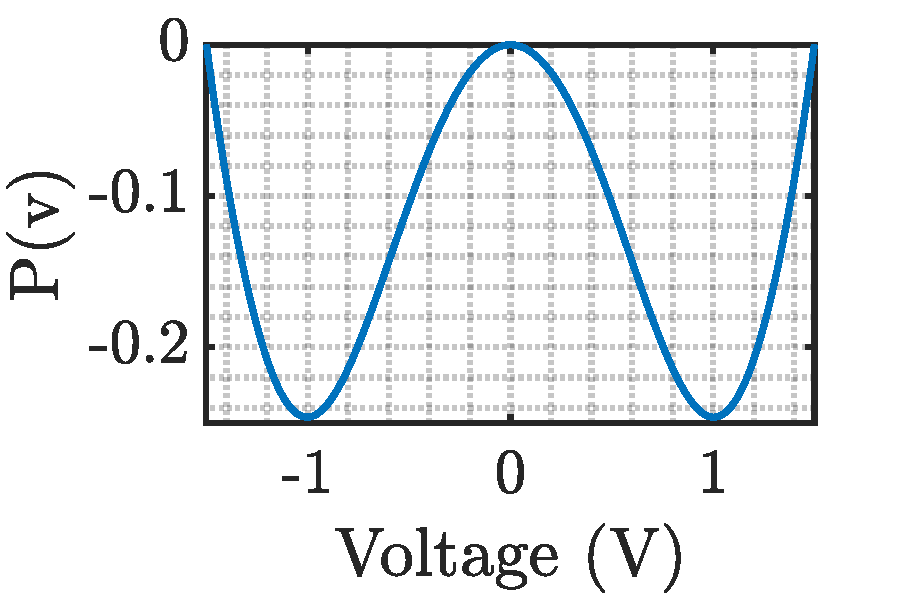
\includegraphics[width=0.4\textwidth]{double_well.pdf}
%     \caption{\fixme{double well of the -P(v)}}
%     \label{fig:double_well}
% \end{figure}

%Since function $H(v)$ satisfies the conditions in Eq.
%\ref{eqn:H_partials} for all $i's$ representing a sufficient condition
%for $\frac{dH(v)}{dt}=-\sum_{i}\frac{\partial H(v_i)}{\partial
%v_i}\frac{dv_i}{dt}\leq0$, the system is stable in the Lyapunov sense and it
%is guaranteed to converge to a minimum of $H(v)$.

Note that this analysis does not guarantee that the system will converge to a
\emph{global} minimum as it depends on the energy landscape and initial 
conditions. This is similar to other annealers: None 
has strong guarantees for reaching ground state in a typical usage scenario
(as opposed to ideal conditions) or in an efficient manner. For example, it
is shown that simulated annealing can reach ground state in a system with
a finite phase space. However, the time it takes to do so may be longer than
enumerating the space~\cite{varty2017simulated}.
\end{comment}

\section{Experimental Analysis}
\label{sec:evaluations}

In this section, we discuss the experimental analysis of our design by describing the experimental methodology and comparing our system to existing LDPC decoders in solution quality, throughput, and energy consumption. 
These decoders can be implemented using GPUs, FPGAs, or as ASICs and are often 
explicitly designed to a particular code. We chose 3 implementations representating 
the state of the art ASIC decoders for 5G standards to compare against.

Behavioral simulation of our LDPC decoder's is done by solving Eq.~\ref{eqn:rim_node_simplifed}, 
using MATLAB's nonstiff, single step, 5th-order differential solver (ode45). Circuit parameters are 
obtained using Cadence with 45nm Generic Process Design Kit (GPDK045). 
We also ran a state-of-the-art variant~\cite{Isakov}  of 
Simulated Annealing to obtain solution quality for LDPC decoding using the traditional
QUBO formulation.

%which shows how the capacitor's voltage representing each node changes over time. $J_{ij}$ represents the effective conductance of the coupling with the parity equations. ${J_b}_i$ represents the bias conductance, ${v_b}_i$ represents the bias voltage. %and $v_i$ represents the current voltage on the node.



\begin{comment}
    

\subsection{Benchmarks and Metrics}

They are many standards defining LDPC codes for different applications. Most recently, the LDPC code has been standardized for wireless enhanced-mobile broad-band (eMBB) communication in 5G new radio (NR) by the 3-generation partnership project (3GPP). We use the LDPC codes defined by this standard as our benchmarks to compare the solution quality of different algorithms.

\begin{figure}[htp]
    \centerline{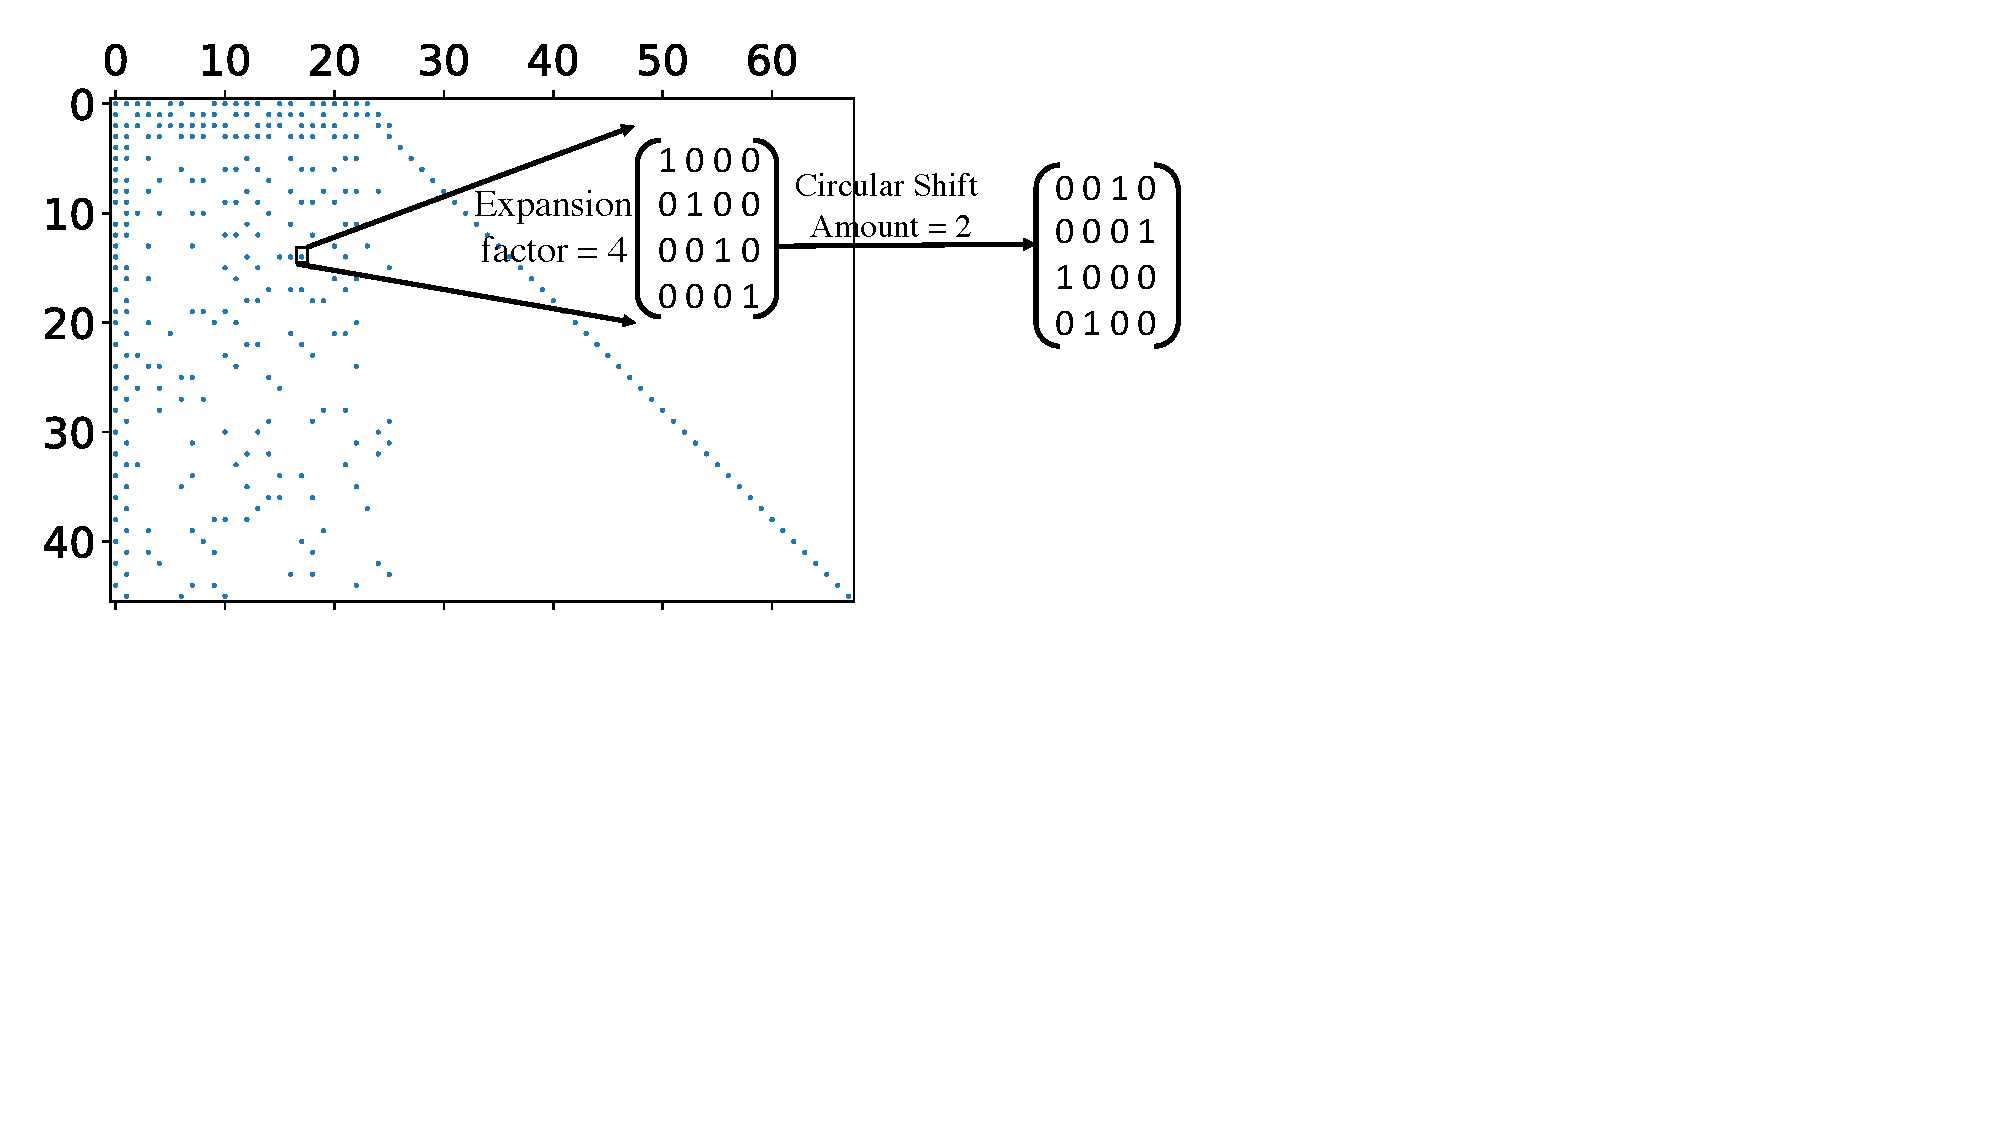
\includegraphics[width=0.47\textwidth]{FIGS/circular_shift.pdf}}
    \caption{Structure of 5G-NR standard base graph 1. Each blue dot represents a nonzero element which will be replaced by a circular identity matrix based on the expansion factor as shown.}
    \label{fig:5g-nr}
\end{figure}

\subsubsection{5G-NR standard} \label{sec:5g_nr_standard}
 The 5G standard describes two base-graph (BG) matrices: BG1 and BG2, which are used to construct a parity check matrix. Figure~\ref{fig:5g-nr} shows the structure of BG1. The blue dots in the figure~\ref{fig:5g-nr} show nonzero elements of the matrix. It has 46 rows and 68 columns, and the BG2 matrix has 42 rows and 52 columns. Rows in the base graphs describe parity check equations. By default, BG1 generates an LDPC code with a rate equal to $1/3$, and BG2 generates an LDPC code with a rate equal to $1/5$. Based on the required rate, we chose the base graph. 

Once the base graph is chosen, each zero entry is replaced with a $Z \times Z$ all-zero matrix. Each nonzero entry is replaced with a $Z \times Z $ circular shifted identity matrix. $Z$ is called an expansion factor. The amount of circular shift depends on the value of the nonzero element. The values of the nonzero elements range from 0 to z. If the value is 0, replace the element with the $Z \times Z$ identity matrix; otherwise, circularly shift the identity matrix based on the value. In figure ~\ref{fig:5g-nr} an example with an expansion factor of 4 and the circular shift amount of 2 is shown. The 5G-NR standard allows different discrete expansion factors ranging from 2 to 384. For any further details please refer to the following paper~\cite{bae2019overview}.

\subsubsection{Metrics}

To compare the solution quality of different algorithms, we use a metric called Bit Error Rate (BER). It defines the probability of a bit being erroneous; mathematically, it is defined as the ratio of the number of error bits by the total number of bits. The number of error bits is equal to the Hamming distance between the decoded and original message. Lower is better.

%The LDPC decoders are designed for different standards based on other design principles using alien technology. So we decided to use $Gbits/sec/Watt$ as the final figure of merit for comparison among different LDPC decoders

%\subsection{Architectural details for 5G-NR standards}\label{sec:5g-nr}
\end{comment}



%\subsection{Comparison with existing LDPC decoders}

\begin{comment}
\begin{table*}[htb]
\centering
\caption{comparison of hybrid LDPC decoder with existing decoders}
\label{table:comparision}
%\resizebox{\columnwidth}{!}
{
%\setlength{\tabcolsep}{4pt}
\begin{tabular}{|c|c|c|c|c|c|c|} 
\hline
\bf {Design\textbackslash Decoder} & \thead{~\cite{schlafer2013new}}  & \thead{~\cite{lin202133}} & \thead{~\cite{cheng2014fully}}   & \thead {~\cite{lee2022multi}}  & \thead{~\cite{thi2021low}} & \thead{this work}\\  
\hline\hline

CMOS Technology  &   65nm LVT  & 28nm & 90nm   & 65nm  & 65nm & 45nm\\ 
\hline
Standard        &  IEEE802.11ad   & 5G-NR   & -    &5G-NR & 5G-NR & 5G-NR \\ 
\hline
Decoding Algorithm & Min-Sum & \thead{ Normalized\\Min-Sum}   &  \thead{ Normalized\\Min-Sum}  & \thead{ offset\\Min-Sum} & \thead{Combined \\ Min-Sum} & \thead{hybrid \\ Ising model}  \\
\hline
Block size         &  672  &  \thead{all cases of 5G}  & 2048 & \thead{all cases of 5G} & 3808 & \thead{all cases of 5G} \\
\hline
\thead{Decoding Latency \\(iterations or annealing time) }  &  10 & 5 &  9 & 3 &10 & 0.22 $\mu sec$\\
\hline
Max Throughput (GBs/sec) & 160.8 & 6.7  & 45.09  & 21.78 &3.04 & 118.6 \\
\hline
Max Power (mW)    & 5360 & 232 & 1110 & 413 & 259 & 1566 \\
\hline
Area ($mm^2$) &   12.09  & 1.97 & 9.6 & 5.74 & 1.49 & 33\\
\hline
Energy (pJ/bit)  & 36.1 & 145  & 20.33  & 94.89 & 85.2& 13.14\\

%\hline
%Gbits/Sec/$mm^2$  & 13.30 & 3.4  & 4.7  & 3.82 & 2.04& -\\
%\hline

\hline
\end{tabular}
}
\end{table*} 
\end{comment}

\subsection{Comparison with existing LDPC decoders}
\begin{comment}
\begin{table*}[htb]
\centering
\caption{comparison of hybrid LDPC decoder with existing decoders}
\label{table:comparision}
%\resizebox{\columnwidth}{!}
{
%\setlength{\tabcolsep}{4pt}
\begin{tabular}{|c|c|c|c|c|c|} 
\hline
\bf {Design\textbackslash Decoder} & \thead{~\cite{schlafer2013new}}  & \thead{~\cite{lin202133}}   & \thead {~\cite{lee2022multi}}  & \thead{~\cite{thi2021low}} & \thead{this work}\\  
\hline\hline

CMOS Technology  &   65nm LVT  & 28nm   & 65nm  & 65nm & 45nm\\ 
\hline
Standard        &  IEEE802.11ad   & 5G-NR & 5G-NR & 5G-NR & 5G-NR \\ 
\hline
Decoding Algorithm & Min-Sum & \thead{ Normalized\\Min-Sum}   &  \thead{ offset\\Min-Sum} & \thead{Combined \\ Min-Sum} & \thead{hybrid \\ Ising model}  \\
\hline
Block size         &  672  &  \thead{all cases of 5G}  & \thead{all cases of 5G} & 3808 & 1088 \\
\hline
\thead{Decoding Latency per iteration\\ (nsec)} &  4  & 787 & 1530  & 125.33  & 220  \\
\hline
\thead{Max Throughput per iteration \\(GBs/sec)} & 160.8 & 33.2  & 17.06 & 30.38 & 4 \\
\hline
Max Power (mW)    & 5360 & 232  & 413 & 259 & 6.59 \\
\hline
Area ($mm^2$) &   12.09  & 1.97  & 5.74 & 1.49 & - \\
\hline
Energy (pJ/bit) per iteration  & 36.1 & 29  & 24.2 & 8.52 & 1.33\\
\hline
\thead{BER @ SNR 3 \\ exp\_factor = 16 \\ bit width =8bits }  &  5.69E-02 & \red{3.67E-02}  & 3.67E-02 & \red{3.67E-02} & 1.61E-02\\
\hline
\end{tabular}
}
\end{table*}

\todo{block size must be the same, increase either area or latency to compensate for the block size, equation}

\end{comment}

\begin{table}[htb]
\centering
\caption{Comparison of the proposed LDPC decoder with existing decoders, all parameters are adjusted to implement highest expansion factor}


%\donotshow{
%}

\label{table:comparision}
\resizebox{\columnwidth}{!}{
\setlength{\tabcolsep}{4pt}
\begin{tabular}{|c|c|c|c|c|} 
\hline
\bf {Design\textbackslash Decoder}  & \thead{~\cite{lin202133}}   & \thead {~\cite{lee2022multi}}  & \thead{~\cite{thi2021low}} & \thead{this work}\\  
\hline\hline

CMOS Technology    & 28nm   & 65nm  & 65nm & 45nm\\ 
\hline
Standard          & 5G-NR & 5G-NR & 5G-NR & 5G-NR \\ 
\hline
Decoding approach & \thead{ Normalized\\Min-Sum}   &  \thead{ offset\\Min-Sum \\ (OMS)} & \thead{Combined \\ Min-Sum} & \thead{Augmented \\ Ising machine}  \\
\hline
Block size         &  26112 & 26112 & 3808 (26112$^*)$  & 26112 \\
\hline
\thead{Decoding Latency per iteration\\ (nsec)}  & 787 & 1530  & 125.33 (860$^*)$  & 320  \\
\hline
\thead{Max Throughput per iteration \\(Gbs/sec)}  & 33.2  & 17.06 & 30.38 & 81.6 \\
\hline
Max Power (mW)     & 232  & 413 & 259 & 158.24 \\
\hline
Area ($mm^2$)  & 1.97  & 5.74 &  1.49 & 5.44 \\
\hline
Energy (pJ/bit) per iteration   & 29  & 24.2 & 8.52 & 1.94\\
\hline
quantization   & 5  & 8  & 4 & 8\\
\hline
%\thead{BER \\  SNR = 2 \\exp\_factor = 64}   & - & - & - &-\\
%\hline
\end{tabular}
}
\footnotesize *Latency scaled for direct comparison with other designs.
%\todo{change xxx and yyy to original paper numbers}
\end{table}


\subsubsection {Comparison with ASIC LDPC decoders}
Table~\ref{table:comparision} shows a detailed comparison of our work with existing ASIC LDPC decoders. 
The decoders are designed for 5G standards.~\cite{lin202133},~\cite{lee2022multi} support all the LDPC codes described by the 5G standards, whereas~\cite{thi2021low} is designed for a particular code created by a specific expansion factor.~\cite{thi2021low} reported their parameters for a decoder intended for an expansion factor of 56. We have modified its decoding latency to represent the decoder designed for an expansion factor of 384 by keeping area and power constant—all the other parameters are directly obtained from the corresponding papers. The table shows that our physical computation-based decoder consumes 4.4 times less energy per bit than the state of the art. Finally, earlier work using Ising machine for LDPC decoding achieves only 21Mb/s~\cite{kasi2020towards}.

\begin{comment}
These ASIC LDPC decoders use different standards and different technologies. They are designed by hard-wiring different variations of the Min-Sum algorithm. 

We designed our BRIM-based LDPC decoder to implement all the codes defined by the 5G-NR standards. The maximum expansion factor allowed by 5G standards is 384, and the maximum number of columns and rows are 68 and 46, respectively. If we construct a code using these factors, it results in a parity check matrix of size $17664 \times 26112$. Suppose we choose a naive design to accommodate this parity check matrix. In that case, we require a system with $26112$ nodes and $17664 \times 26112 = 461242368$ parity units. As described in section~\ref{sec:5g_nr_standard}, the nonzero elements are replaced by a circular shift identity matrix. So even if we consider all $46 \times 68$ matrix to be nonzeros, maximum, we require $46 \times 68\times 384=1024512$ parity units. So to reduce the space and energy, we designed our system with $26112$ rows but $46$ columns. Each row would represent a node, and each column would represent $384$ parity equations. To represent these parity equations, we need $384\times 2$ different wires in each column. If we layout our chip with 45nm technology using four metal layers, 27 $\mu$m wide~\footnote{According to the following paper~\cite{sicard2011introducing} in 45nm technology in metal layers, 1 to 4, the wire width is 60nm, and the space between wires is 80nm}.
If we consider the parity units to be $1\mu$m in length, then the total area of the chip would be 33$mm^2$ approximately. The total annealing time to decode a code word is $0.22 \mu s$, which results in a throughput of 118.6 Gbits/sec. We calculated the maximum power consumed by this system to be 158.24 mW~\footnote{There are 316 nonzero elements in base graph 1. So only $316X384 = 121344$ parity units will be active for a parity check matrix constructed using an expansion factor of 384.}. Hence from this design, we can at least achieve an order of magnitude reduction in energy consumption per bit when compared to other state of the art designs.

\begin{figure}[htbp]
    \centering
    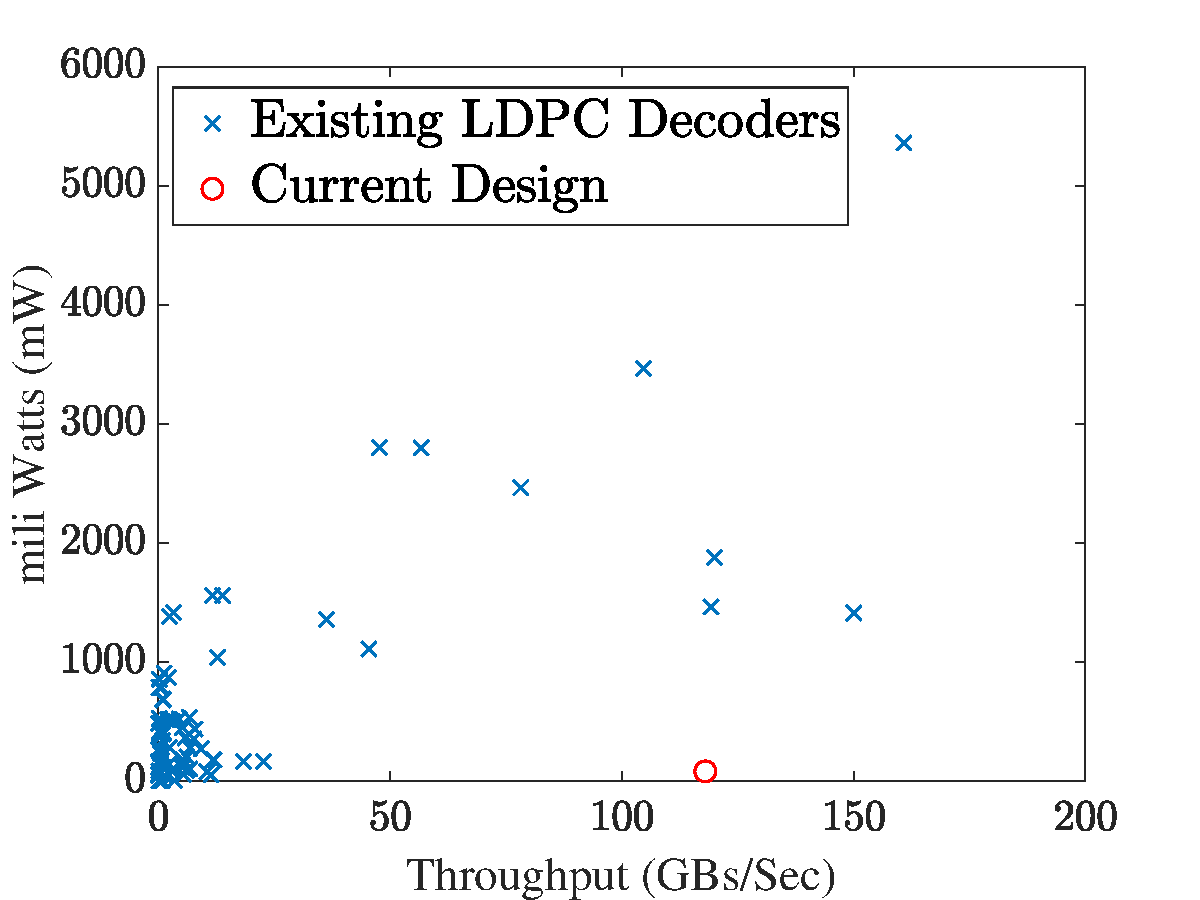
\includegraphics[width=0.45\textwidth]{FIGS/perfomance_ldpc.pdf}
    \caption{Performance vs Power Consumption of various LDPC decoders implemented in literature}
    \label{fig:ldpc_results}
\end{figure}

Figure~\ref{fig:ldpc_results} shows the graph of throughput vs power consumption of ASIC LDPC decoders. The graph is obtained from the following survey papers ~\cite{kingston2021certain,maunder2016survey}. \blue{Even in this graph, all the LDPC decoders are designed with different technology and for different standards. The graph shows that power consumption grows exponentially with the growth in throughput. In our design, parity units are responsible for most power consumption. They grow linear to the expansion factor. Hence, using our design, we could achieve linear growth in power consumption with throughput.}
\end{comment}
%\subsubsection{Comparison with existing Ising machines}

%As discussed in the following section~\ref{?} after conversion, the problem size of 5G-NR LDPC code with an expansion factor of 384 increases to \blue{48769} spins. 

%\todo{need to write}
\begin{comment}

\subsection{Comparison of solution quality of different algorithms }\label{sec:solution_quality}

One thousand messages were encoded using different LDPC codes to obtain the solution quality. These codes were constructed using the 5G-NR standard's base graph 1 with varying factors of expansion. The encoded messages were then modulated using BPSK modulation. The noise was added to the modulated signals based on the signal-to-noise ratio (SNR). These corrupted signals were used to test the different algorithms for solution quality. 

In Figure~\ref{fig:ber} labels 1 to 10 represent the maximum number of iterations used for decoding in the Min-Sum algorithm. QUBO represents the decoding of LDPC codes using QUBO formulation. Modified QUBO represents LDPC decoding using the proposed design. Both modified QUBO and QUBO were annealed for 0.22$\mu$s to obtain BER. The Min-sum algorithm is deterministic, whereas QUBO and modified QUBO are probabilistic. So, we used a different metric called Expected BER to estimate the solution quality. Each message (or instance) was annealed 100 times with random initializations. Each different anneal gives us a different solution. We find the distinct solutions in these different anneals and rank them according to their Ising energies. Considering this order static, the \textit{expected} Bit Error rate (E(BER($N_a$)))~\cite{kim2019leveraging} for each instance is calculated using the formula~\ref{eqn:expected_ber}.

%Figure ~\ref{fig:ber} shows the Bit Error Rate (BER) of different algorithms at different SNR values. The titles of each graph show the expansion factor used for creating the LDPC codes.

\begin{equation}\label{eqn:expected_ber}
\begin{split}
E(BER(N_a)) = \sum_{k=1}^{L} \left[ (\sum_{r=k}^{L} P_I(r))^{N_a} -  (\sum_{r=k+1}^{L} P_I(r))^{N_a}\right] \\ F_I(k)/N     
\end{split}
\end{equation}

 

where N is the number of bits in the message, L is the number of unique solutions obtained by different anneals, r is the rank index of each solution, $P_I(r)$ is the probability of obtaining the $r_{th}$ solution, and $F_I$ is the number of bit errors in the $k^{th}$ solution, relative to the ground truth. The average of 1000 different expected BER is reported as the final Bit Error rate for each SNR. As shown in the figure, modified QUBO gives us the best BER when compared to all the other algorithms.

\begin{figure}[htb]
  \centering
 \begin{minipage}[b]{.40\textwidth}
  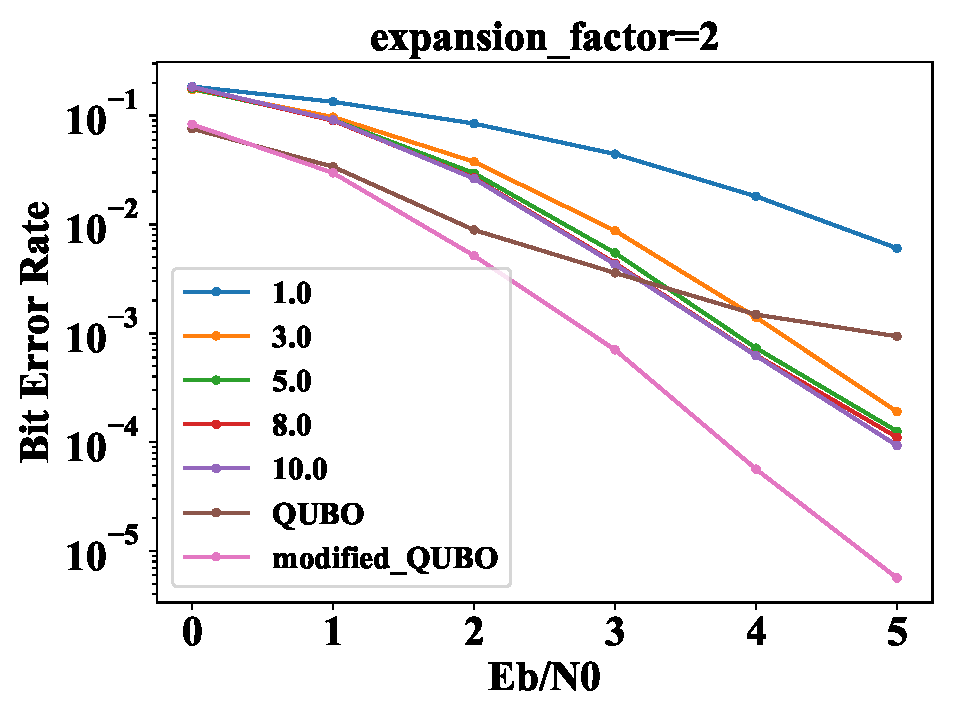
\includegraphics[width=\textwidth]{FIGS/2_.pdf}
  %\caption{This is first figure}
  \end{minipage}%
  \hfill
  \begin{minipage}[b]{.5\textwidth}
  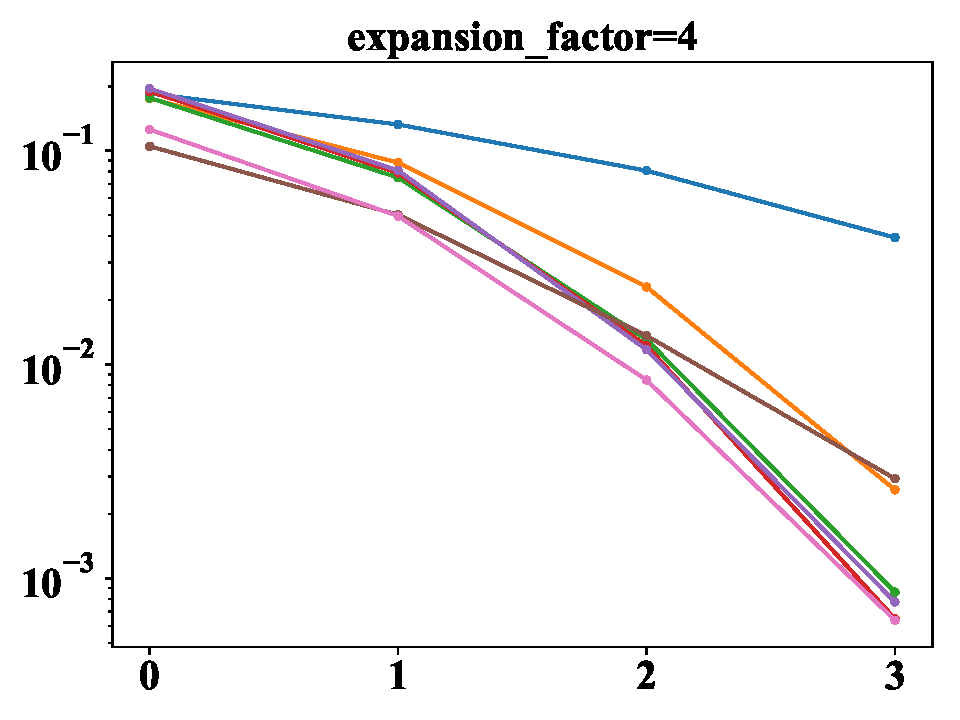
\includegraphics[width = 0.32\textwidth]{FIGS/4_.pdf}
  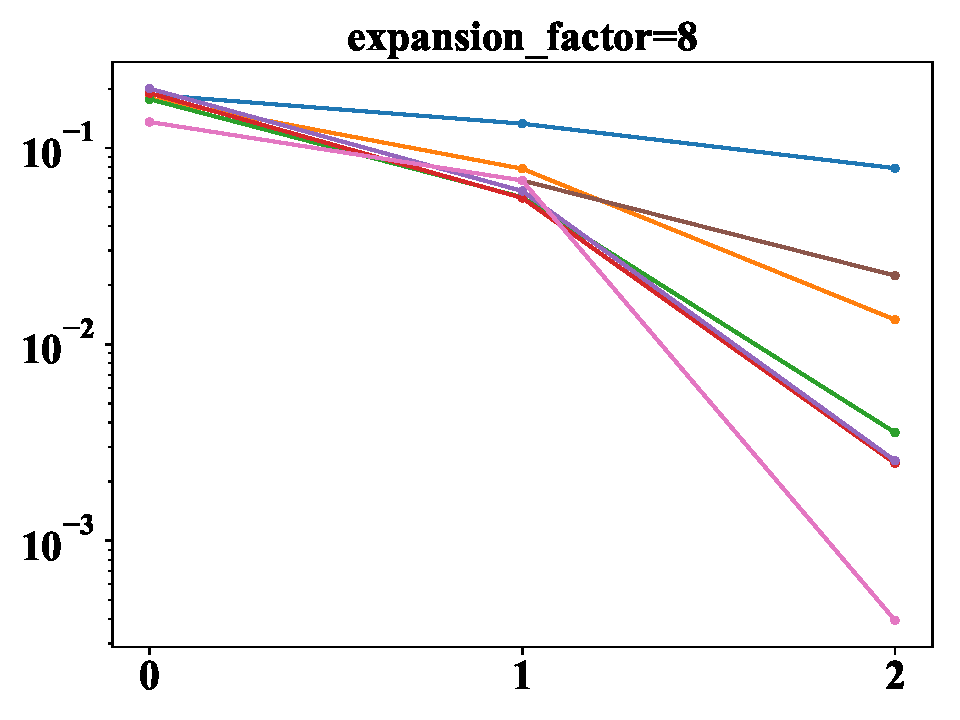
\includegraphics[width = 0.32\textwidth]{FIGS/8_.pdf} 
  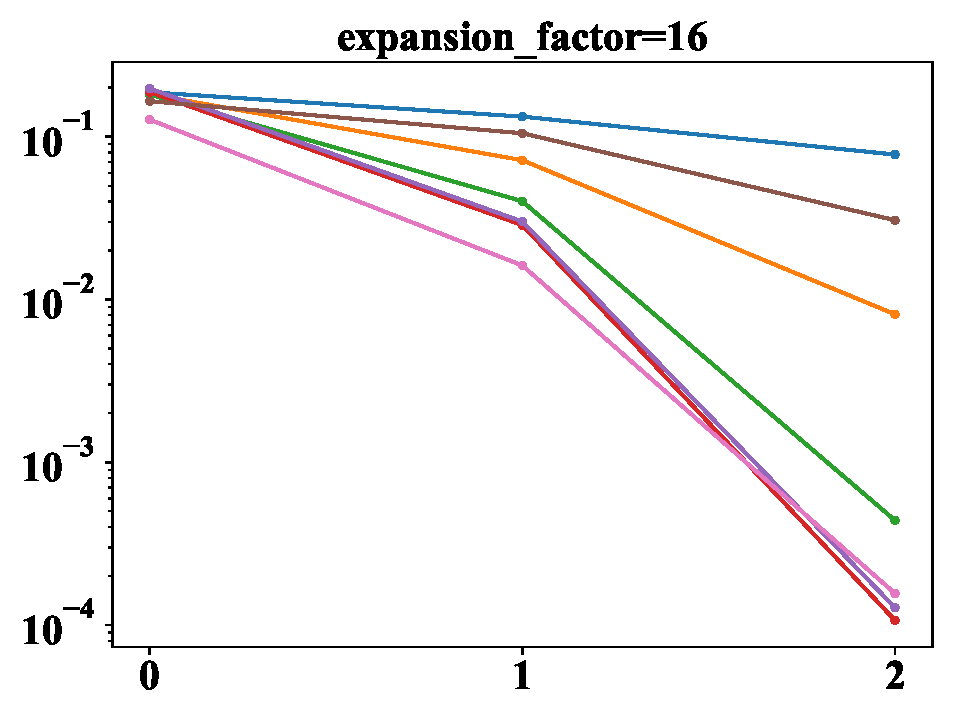
\includegraphics[width = 0.32\textwidth]{FIGS/16_.pdf}
  %\caption{caption}
  \end{minipage} 
  \caption{Bit Error rate achieved by different algorithms at different Signal-noise ratios. Lower the better.}
\label{fig:ber}
\end{figure}

\subsection{Impact of circuit element's noise on solution quality}

\todo{To be implemented}

%\subsection{Circuit Implementation using Cadence}

%\todo{To be implemented}
\end{comment}


\subsection{Comparison with traditional QUBO Formulation }\label{sec:solution_quality}

One thousand messages were encoded using different LDPC codes to obtain the solution quality. These codes were constructed using the 5G-NR standard's base graph 1 with varying expansion factors. The encoded messages were then modulated using BPSK modulation. Noise was added to the modulated signals based on the signal-to-noise ratio (SNR). These corrupted signals were used to test the different algorithms for solution quality. 

Fig.~\ref{fig:ber} shows the solution quality of LDPC decoding using standard QUBO formulations and our proposed formulation (hybrid Ising model or modified QUBO). Since we are analyzing the
quality of the formulation, we use the much faster 
Simulated Annealing (for 10000 iterations) to measure BER. Each message was annealed 10 times with random initializations. Fig.~\ref{fig:ber} shows the average of the bit error rate obtained. We can observe from the graphs that, given the runtime, both the formulations of QUBO yield worse BER compared to our proposed formulation. 

The better performance for our formulation is part of the reason our co-designed
Ising machine performs much better than earlier work using D-Wave annealer.
Additionally, our proposed architecture requires far fewer couplers:
20K couplers (expansion factor 64) vs 
443K and 290K couplers for unary or encoding requires  respectively.

%We find the distinct solutions in these different anneals and rank them according to their Ising energies. Considering this order static, the \textit{expected} Bit Error rate (E(BER($N_a$)))~\cite{kim2019leveraging} for each instance is calculated using the formula~\ref{eqn:expected_ber}.

%\begin{equation}\label{eqn:expected_ber}
%\begin{split}
%E(BER(N_a)) = \sum_{q=1}^{L} \left[ (\sum_{r=q}^{L} P(r))^{N_a} -  (\sum_{r=q+1}^{L} P(r))^{N_a}\right] \\ F(q)/K   
%\end{split}
%\end{equation}
%where K is the number of bits in the message, L is the number of unique solutions obtained by different anneals, r is the rank index of each solution, $P(r)$ is the probability of obtaining the $r_{th}$ solution, $F$ is the number of bit errors in the $q^{th}$ solution, relative to the ground truth and $N_a$ represents number of anneals. The average of 1000 different expected BER is reported as the final Bit Error rate for each SNR. As shown in the figure, modified QUBO gives us the better BER when compared to QUBO formulation.

\begin{figure}[htb]
 \begin{minipage}[b]{.6\columnwidth}
   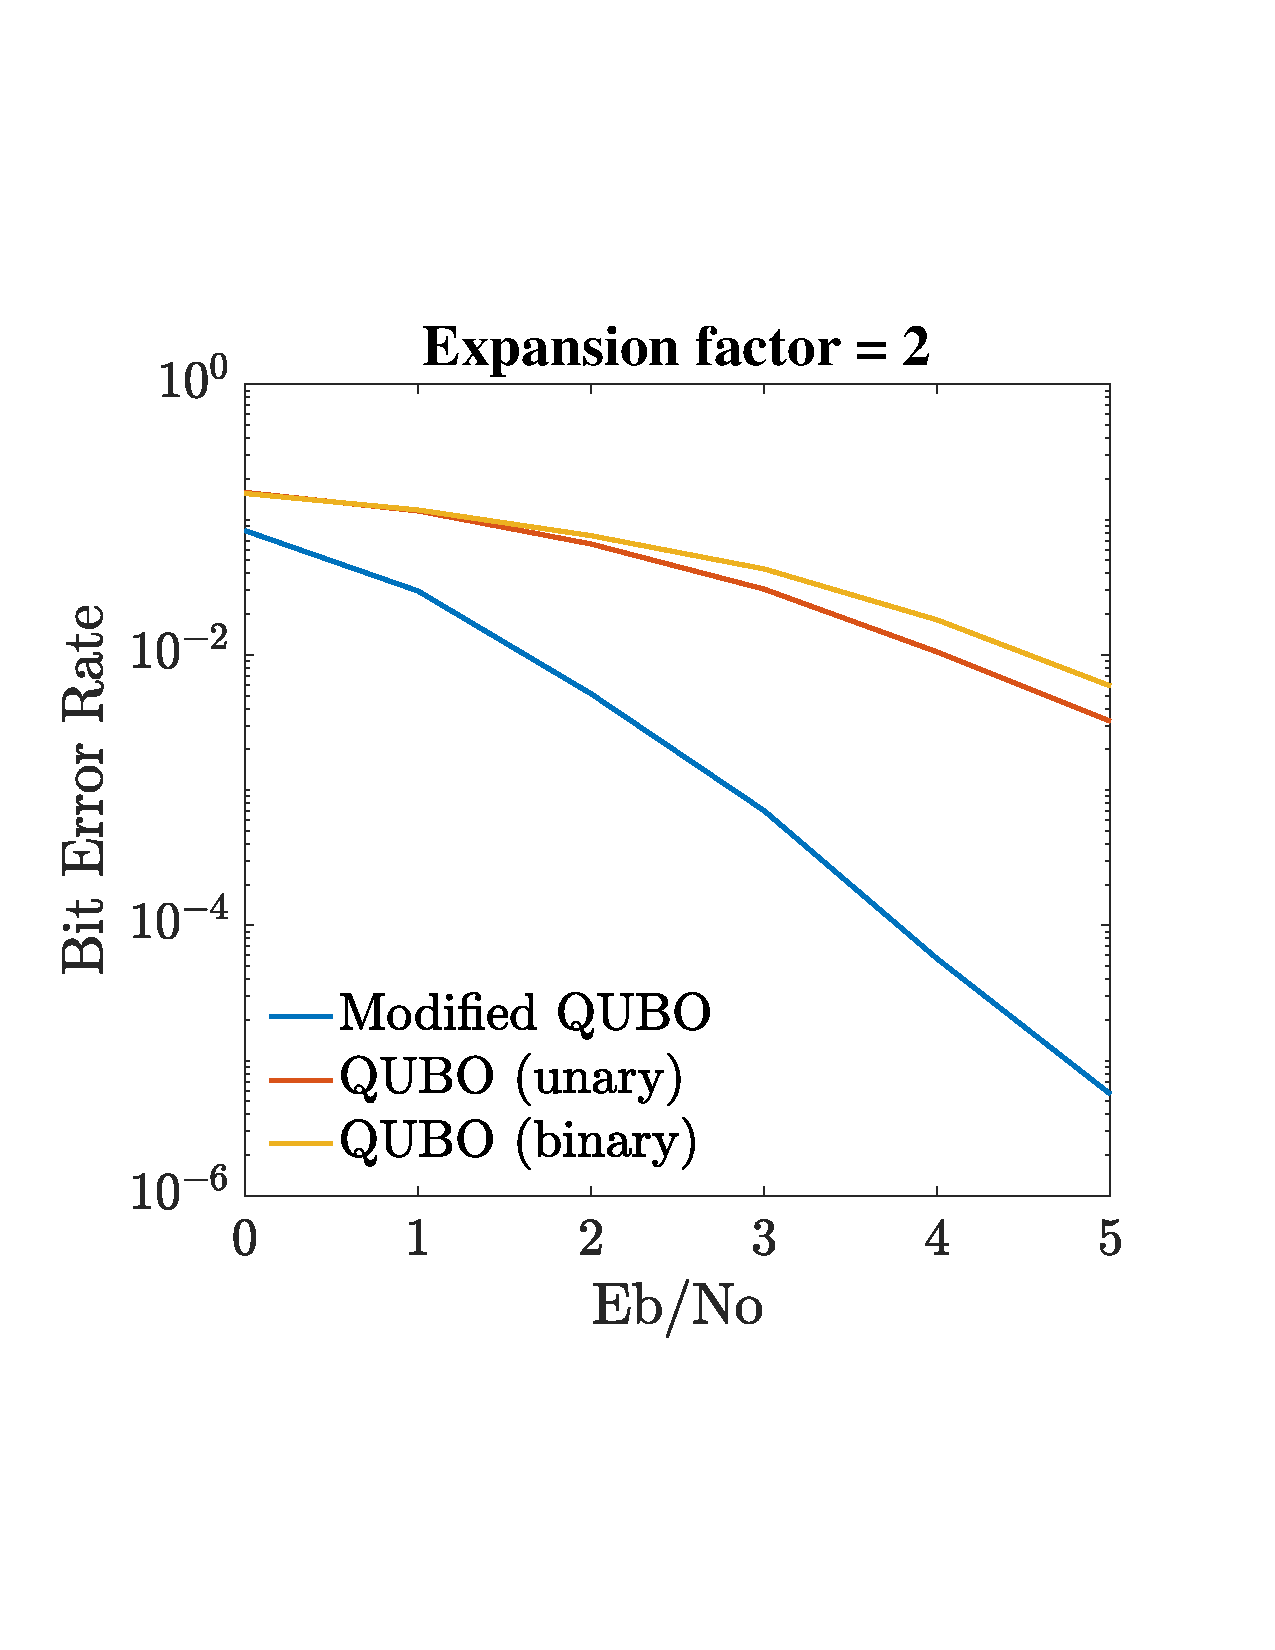
\includegraphics[width =\textwidth]{FIGS/qubo_2.pdf}
  %\caption{This is first figure}
  \end{minipage}%
  \hfill
  \begin{minipage}[b]{.35\columnwidth}
  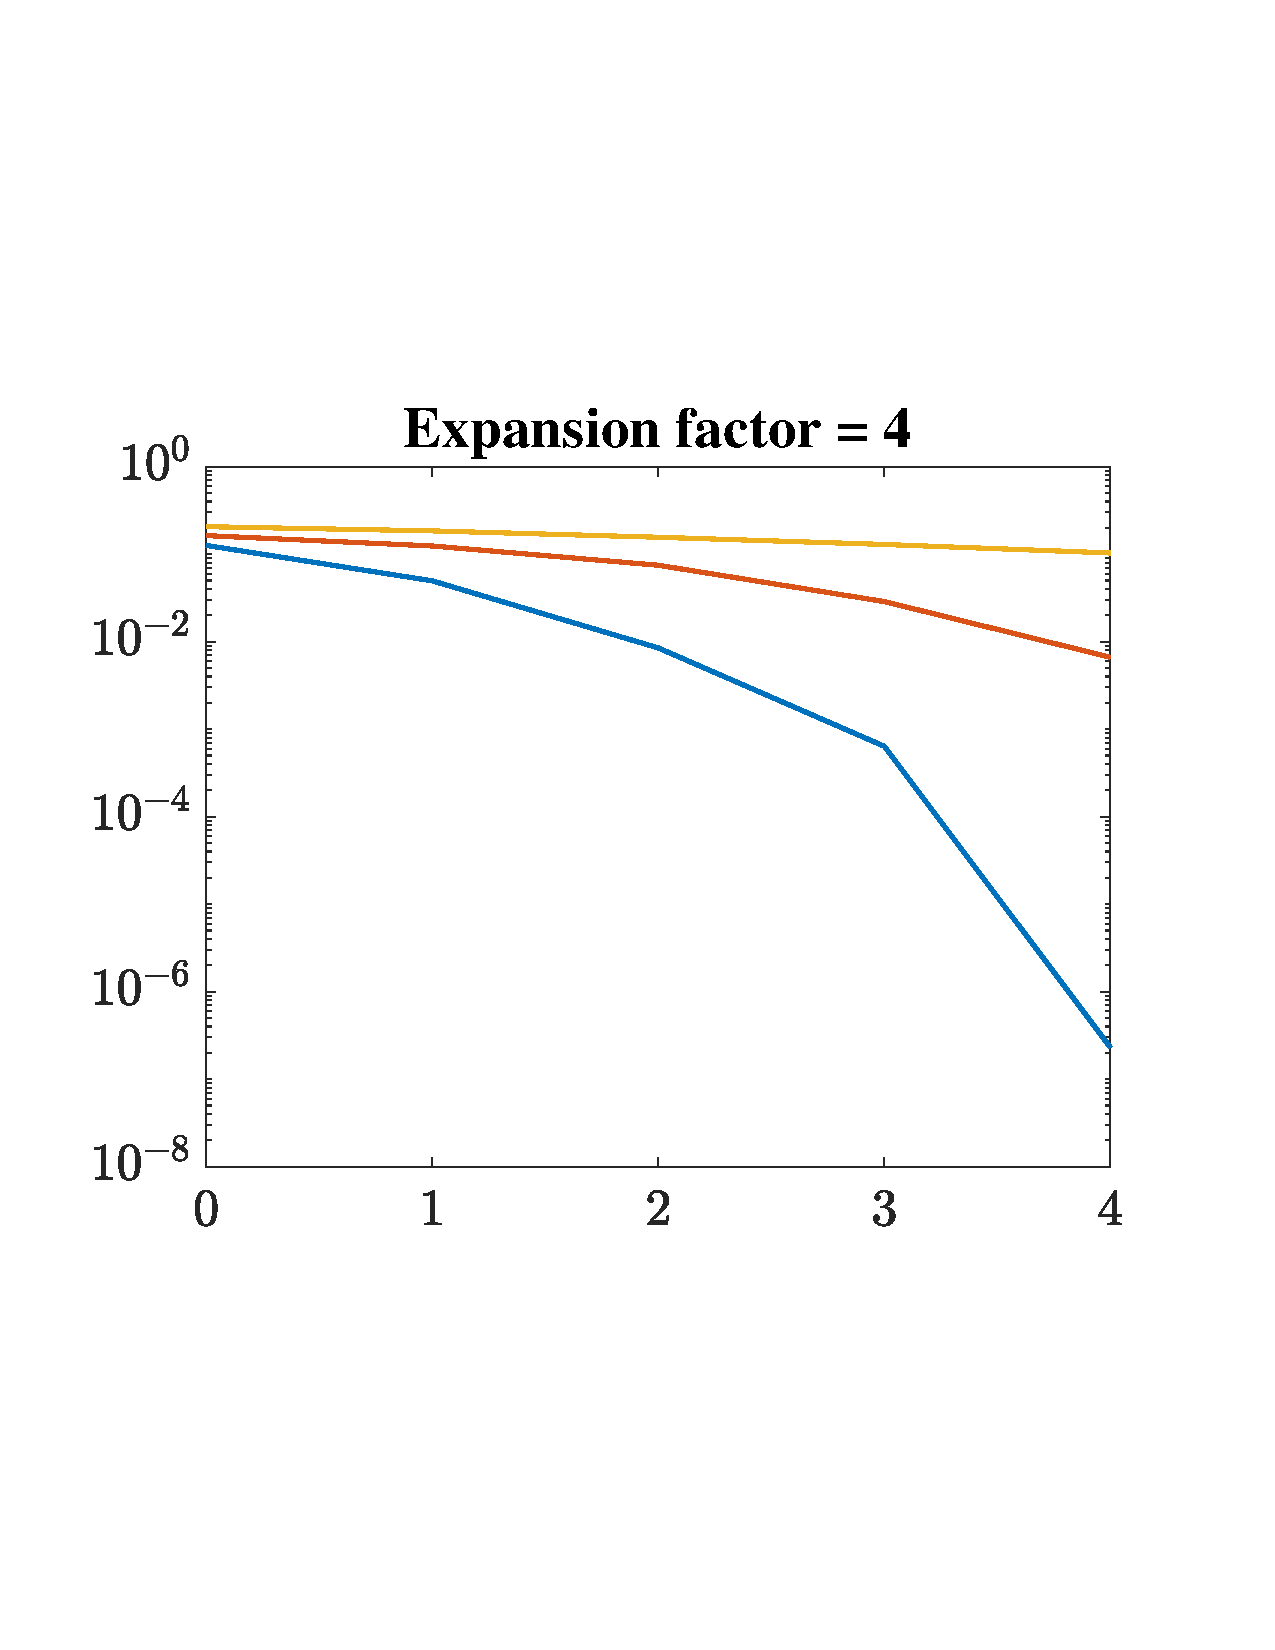
\includegraphics[width = \columnwidth]{FIGS/qubo_4.pdf} 
  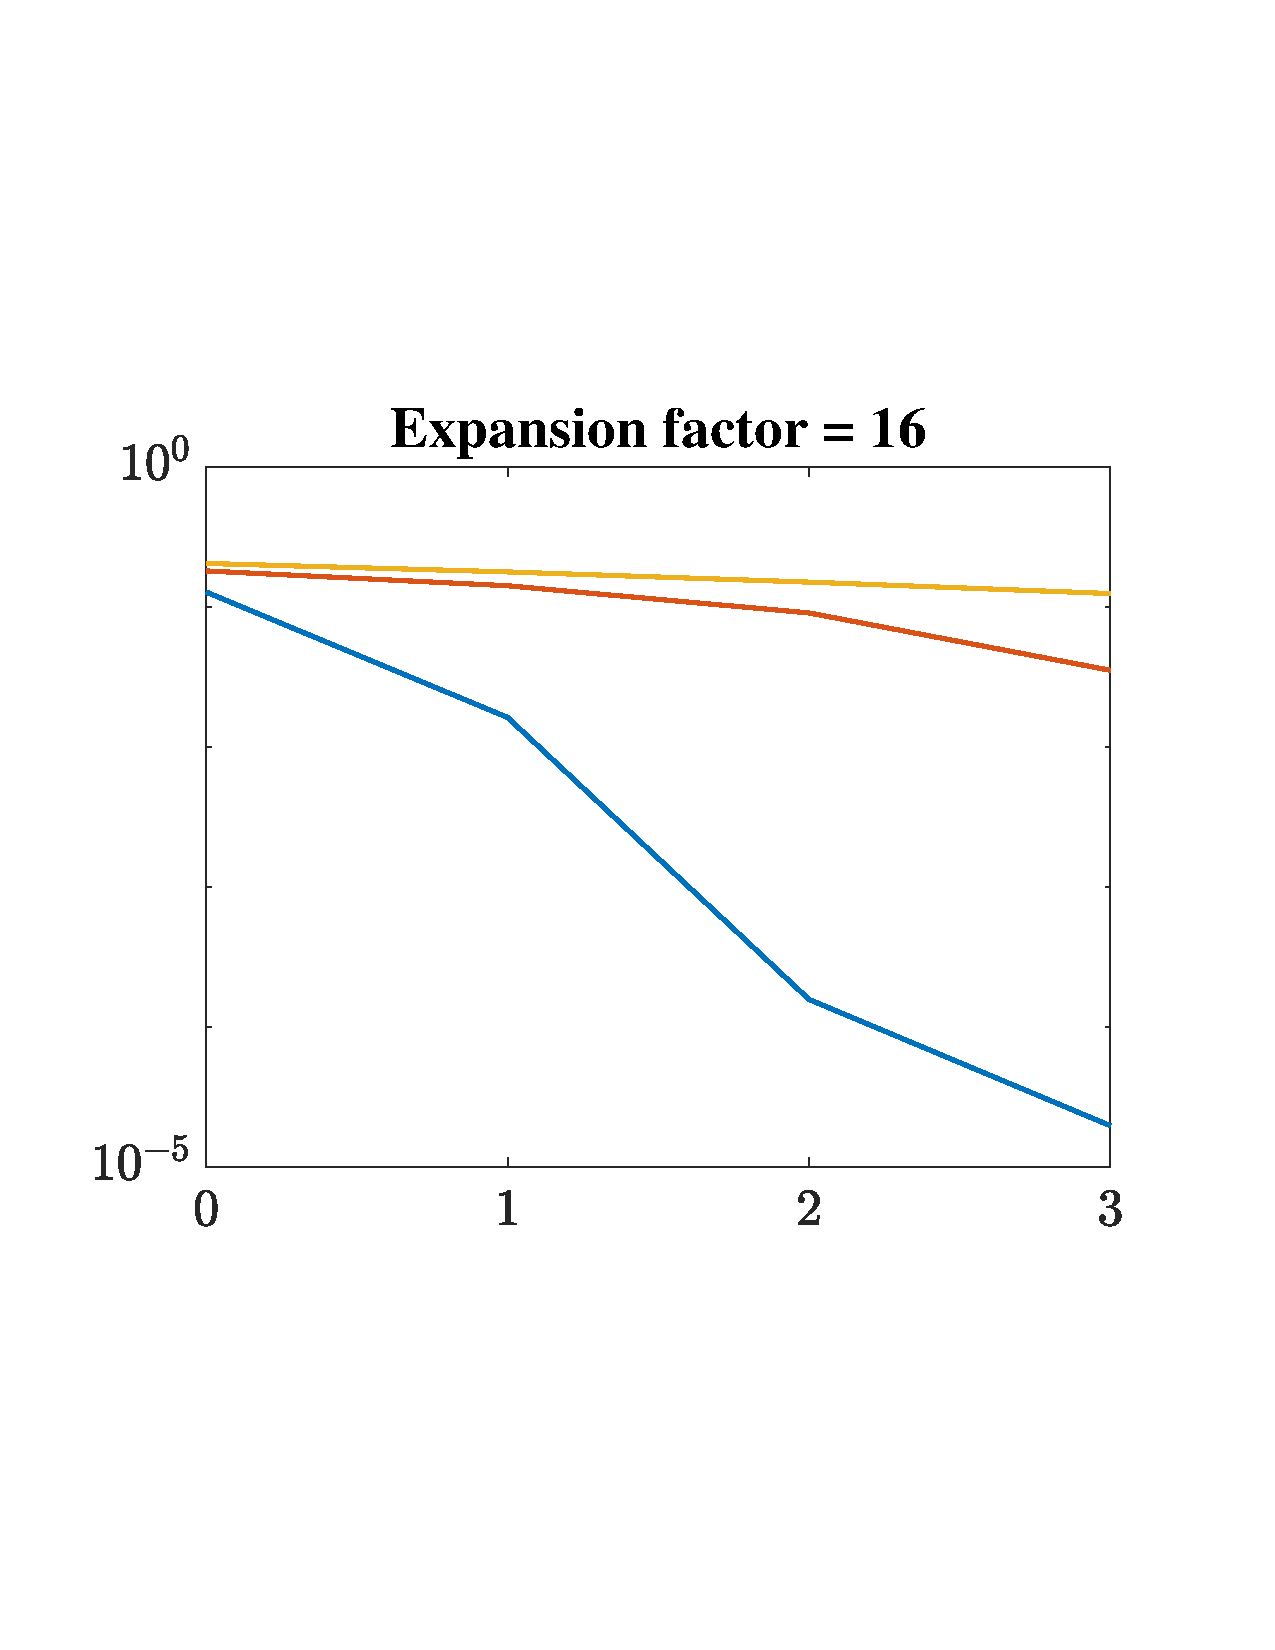
\includegraphics[width = \columnwidth]{FIGS/qubo_16.pdf}
  %\caption{caption}
  \end{minipage} 
  \caption{Bit Error Rate (BER) achieved by different algorithms at different Signal-noise ratios (Eb/No). Lower is better.}
\label{fig:ber}
\end{figure}

\begin{comment}
\begin{figure}[htb]
 \begin{minipage}[b]{.6\columnwidth}
   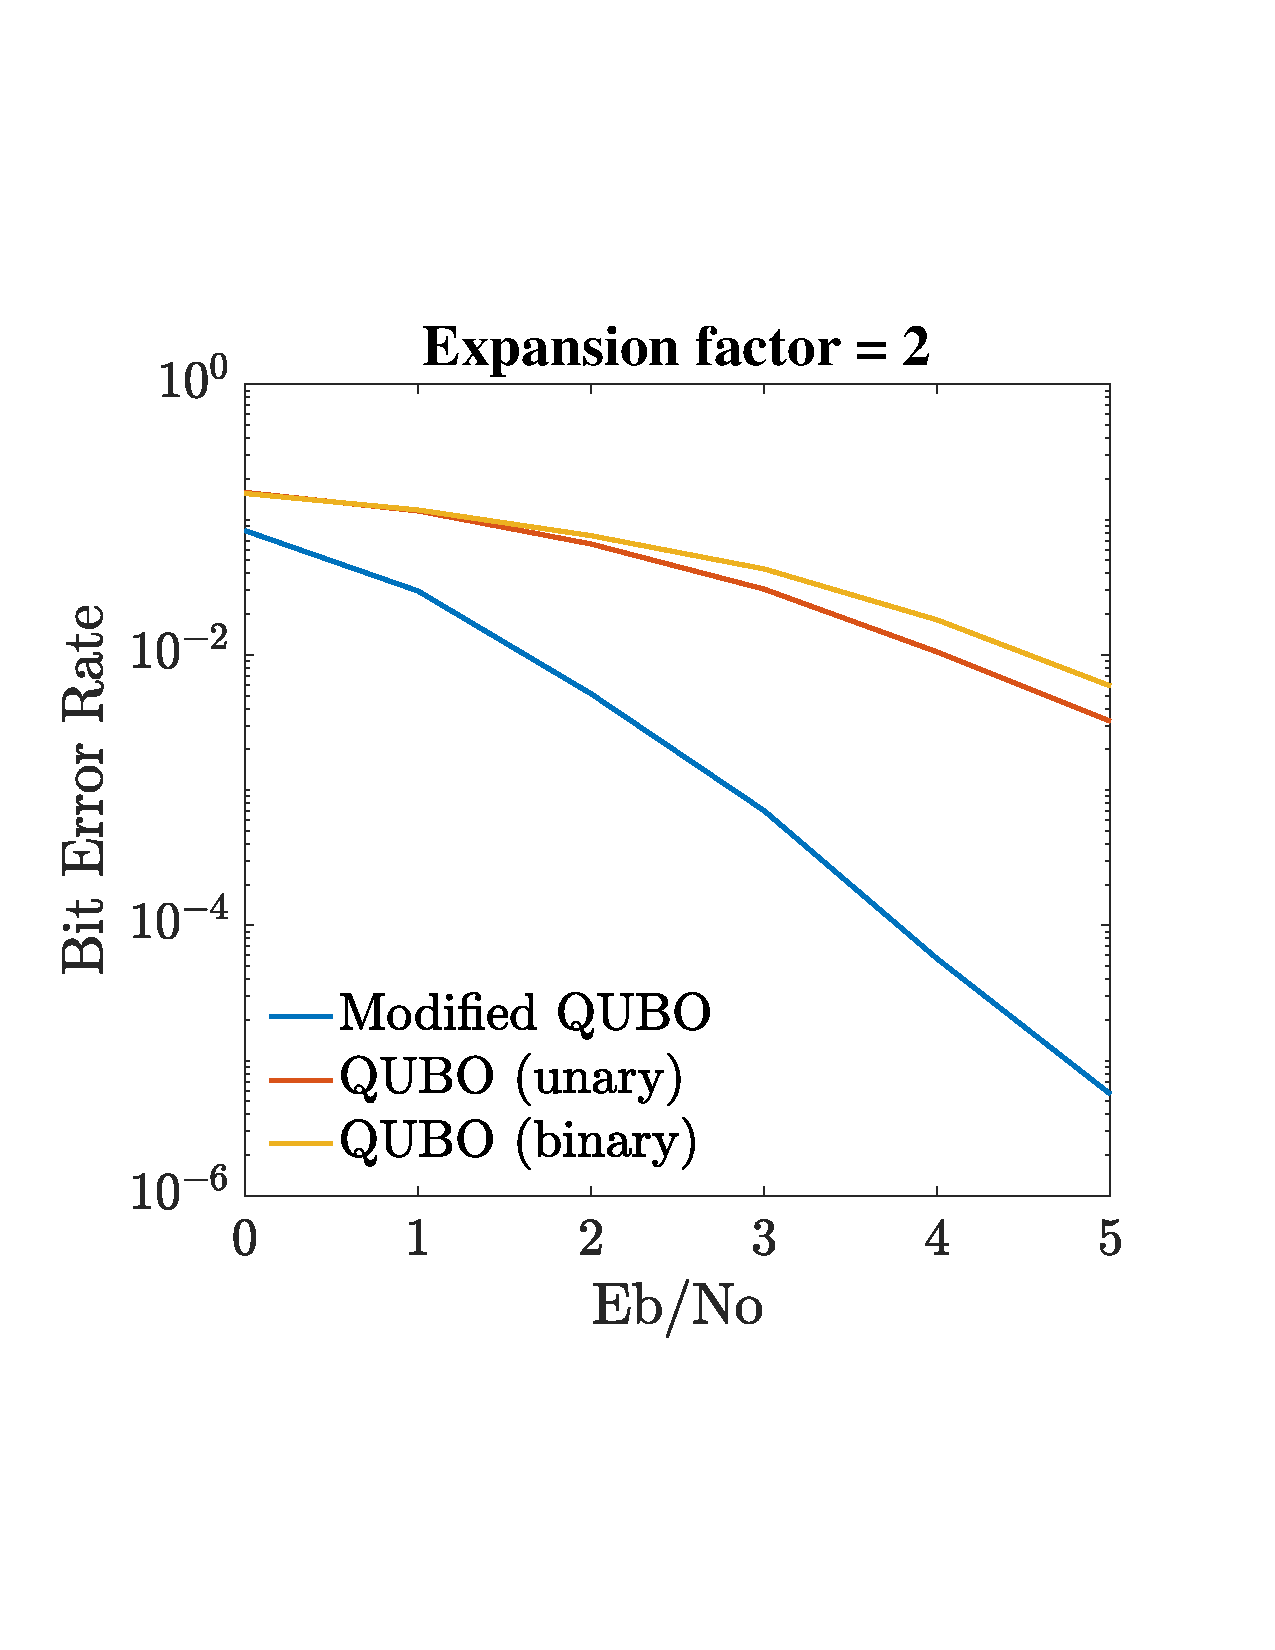
\includegraphics[width =\textwidth]{FIGS/qubo_2.pdf}
  %\caption{This is first figure}
  \end{minipage}%
  \hfill
  \begin{minipage}[b]{.35\columnwidth}
  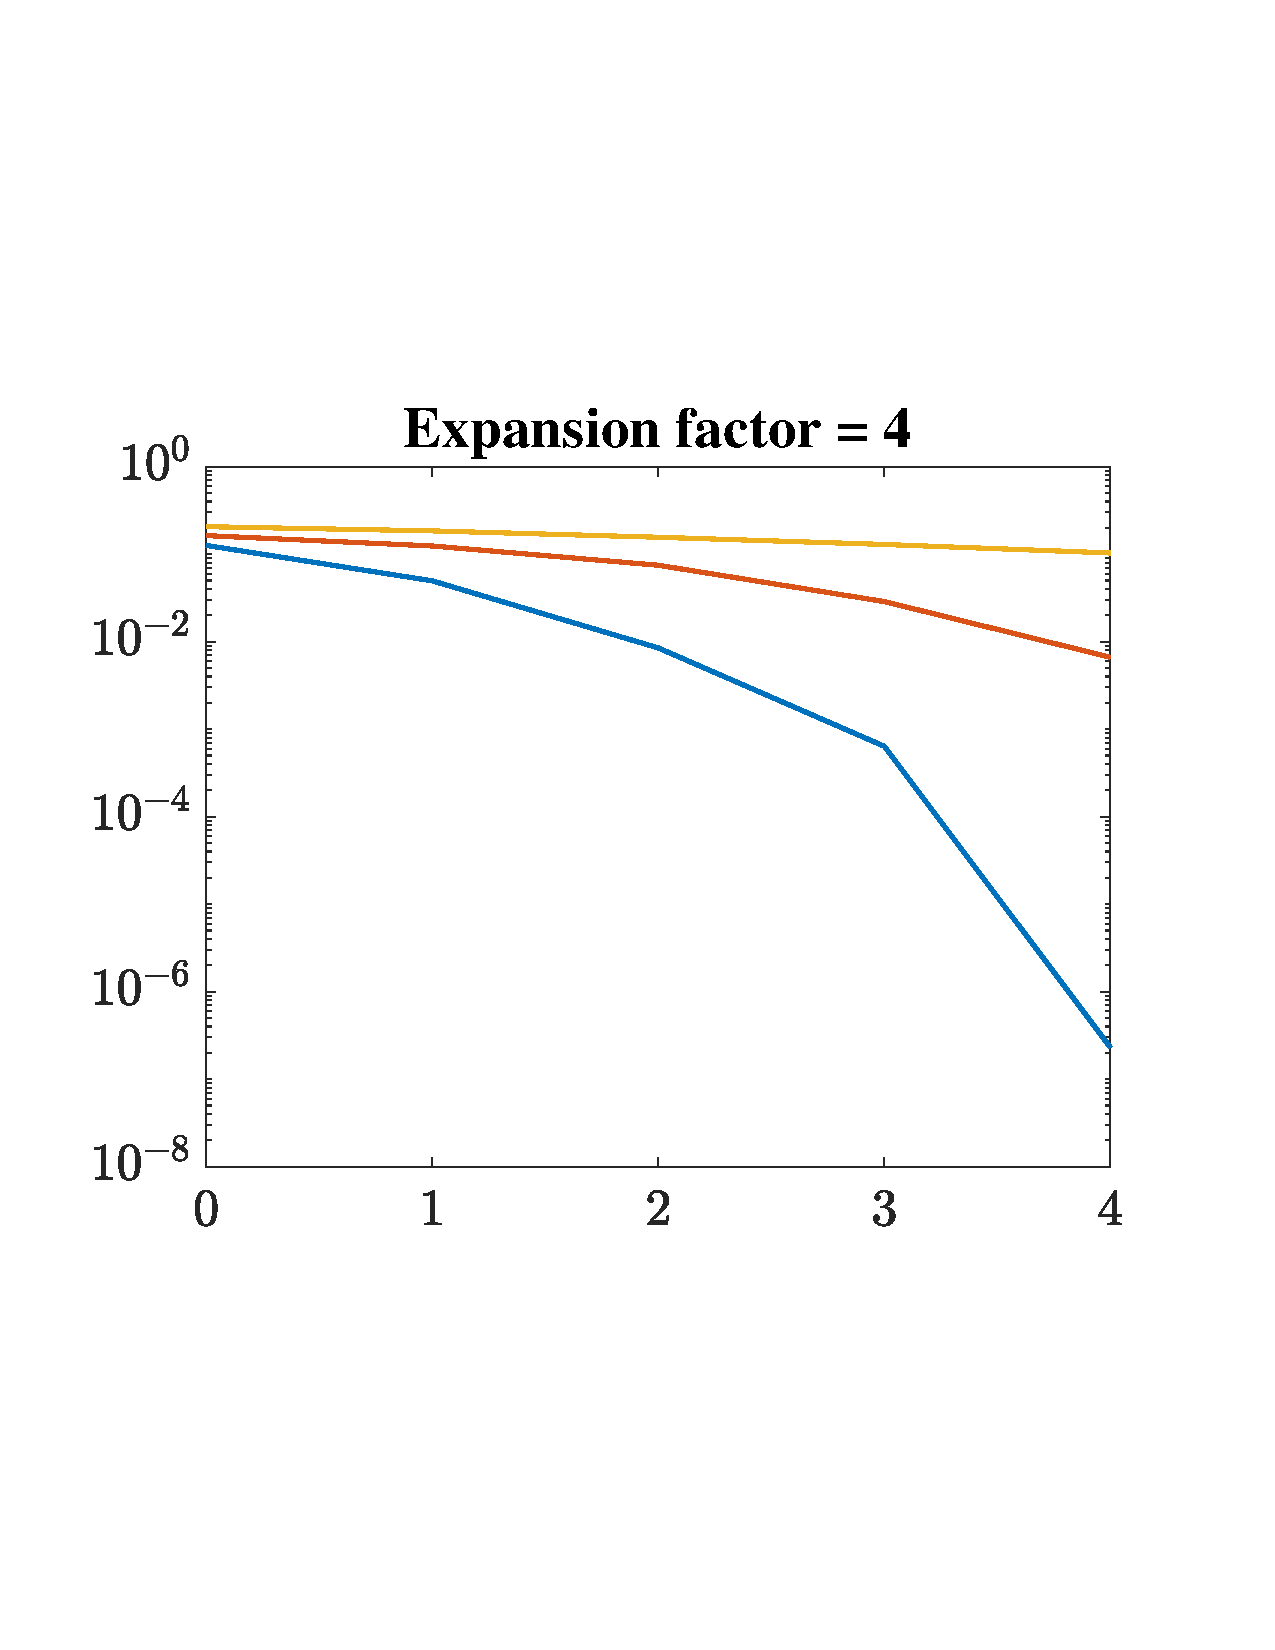
\includegraphics[width = \columnwidth, height=0.72\columnwidth]{FIGS/qubo_4.pdf} 
  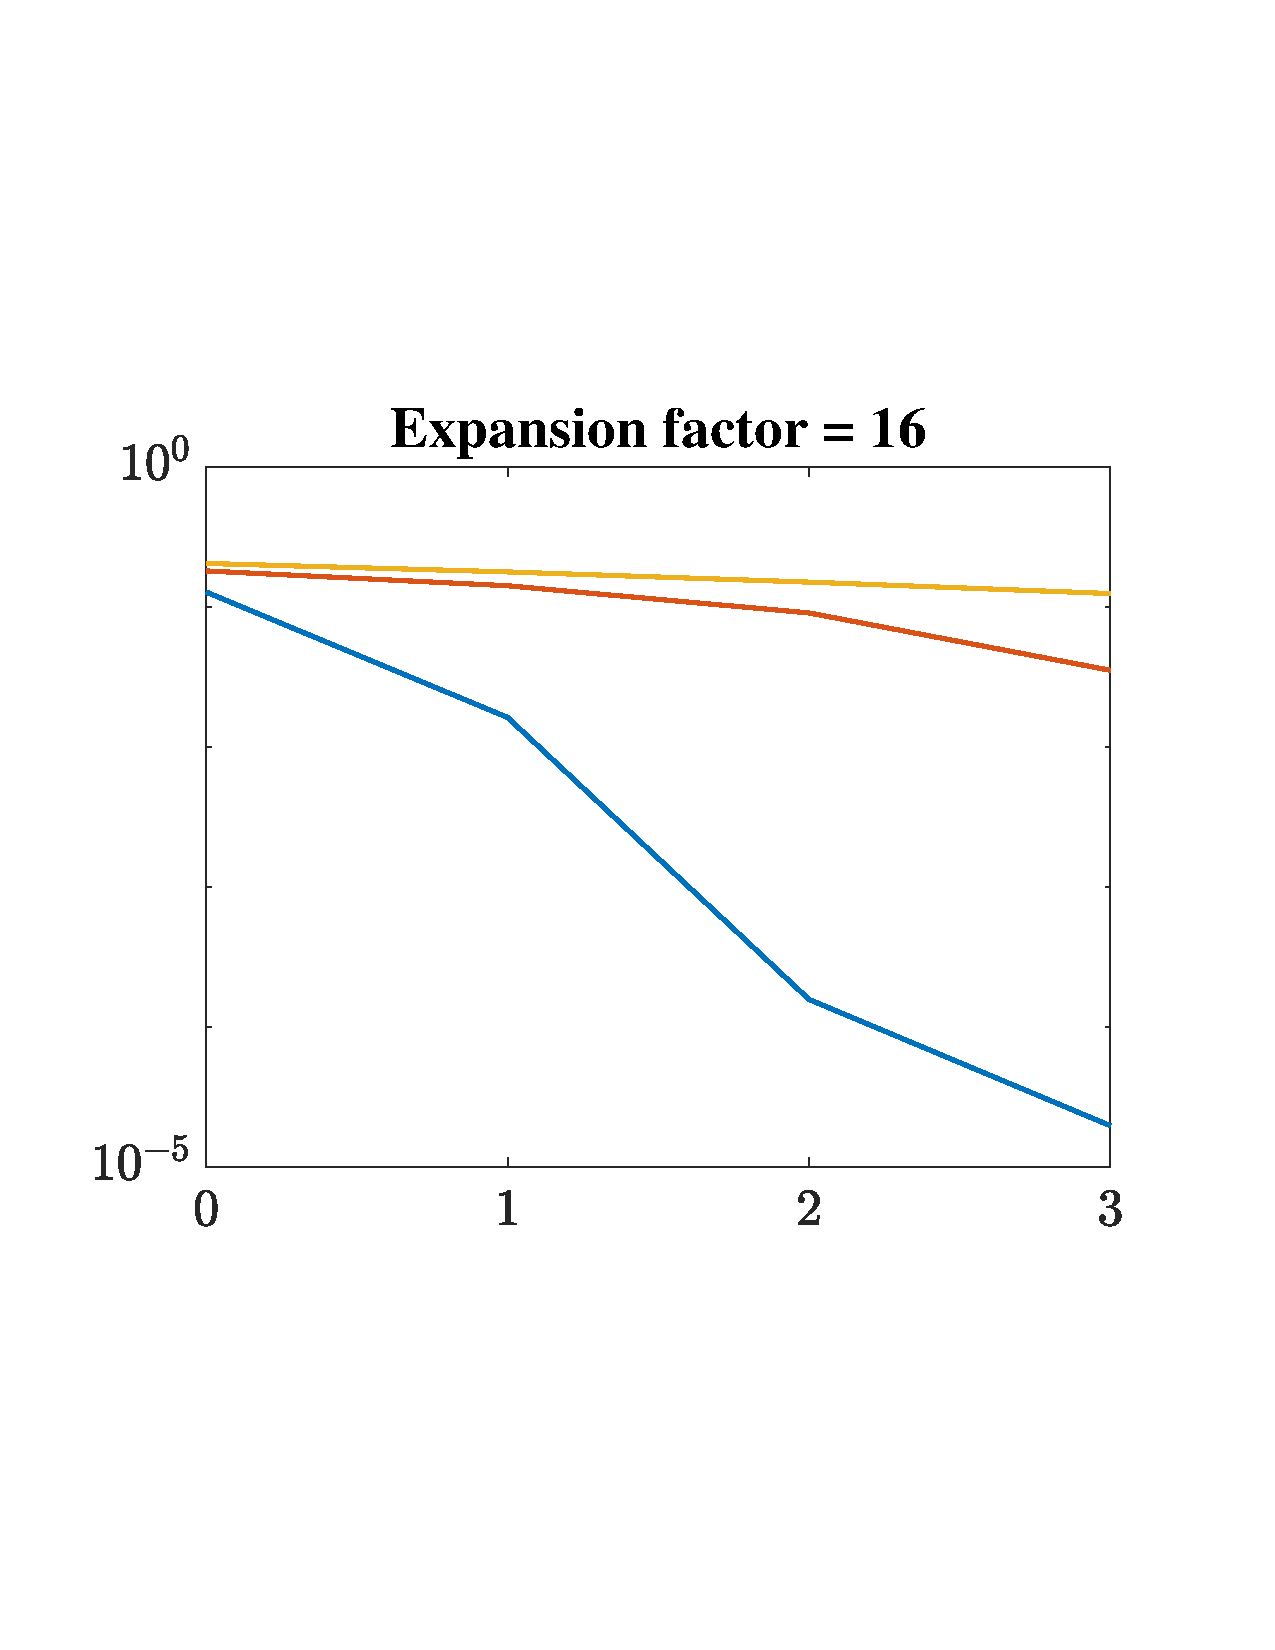
\includegraphics[width = \columnwidth, height=0.72\columnwidth]{FIGS/qubo_16.pdf}
  %\caption{caption}
  \end{minipage} 
  \caption{Bit Error Rate (BER) achieved by different algorithms at different Signal-noise ratios (Eb/No). Lower is better.}
\label{fig:ber}
\end{figure}
\end{comment}

%\todo{needs to be changed}

To compare the solution quality of our proposed design with different variants of belief propagation algorithm, we encoded ten thousand messages using LDPC code constructed using the 5G-NR standard's base graph 1 with an expansion factor of 64. Fig.~\ref{fig:ber_brim} shows the bit error rate obtained by different algorithms. `BP' and `OMS' in the legend represent layered Belief Propagation and layered Offset Min-Sum algorithm, respectively. 
BP and offset Min-sum algorithms were implemented using MATLAB's 5G toolbox. 
We simulate our system evolving for 2.2 $\mu s$. The graph shows that the BER obtained by the hardware approaches the BER rate obtained by BP and its variants at the 7th iteration. 


\begin{figure}[htb]
  \centering
   % 
\includegraphics[width =0.32\textwidth]{LDPC codes/FIGS/ber_sa.pdf}
   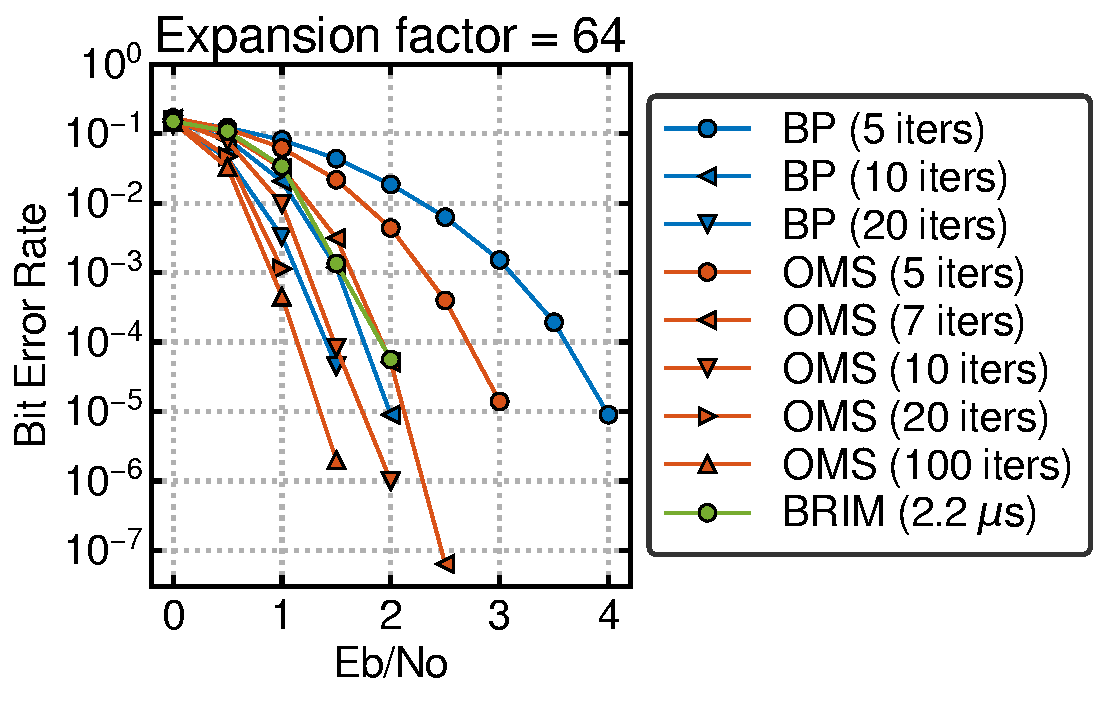
\includegraphics[width=0.50\textwidth]{FIGS/ber.pdf}
  \caption{Bit error rate achieved by different algorithms at different Signal-to-noise ratios. Lower is better.}
\label{fig:ber_brim}
\end{figure}



\input{Sections/5conclusion.tex}

\small
\bibliographystyle{IEEEtran}
\bibliography{main}

%\newpage
%\todo{Find out performance/energy of ``baseline Ising machine" so that we can discuss this improvement in abstract.}
\note{According to the following paper "https://arxiv.org/abs/2007.11069" a 2048 qbit dwave machine can implement a 420bit problem, which can achieve 0.021 gbits/sec  throughput. Whereas state of the art machines achieve 33.2 gbits/sec and we achive 81.6 gbits/sec}

\note{
expansion factor 4, binary;  number of spins: 689 , couplers: 15616; unary, number of spins: 1029 , couplers 25148; actual spins (our model) 272, couplers 1264\\
expansion factor 64, binary; number of spins:11009 ,
Couplers:290688; unary number of spins: 16449, couplers: 443200; acutal spins (our model) 4352.0, couplers 20224.
}

\note{ SNR = power of signal / power of noise; (No units, generally expressed in dB)

$N_0/2$ is the power spectral density of noise;

2W be the bandwidth;

P be the power of signal;

power of noise = $N_0/2*2W$ = $N_0*w$

so SNR = $P/N_0*W$

If 2W is the bandwidth of the signal, Time required to transmit a symbol without interference (T) = $1/2W$ (According to Nyquist rate)

So energy per symbol $(E_s)$ = P*T =  $P/2W$

The energy of noise = variance of noise ($\sigma^2$) = $N_0/2$; (This is derived)

so $E_s/\sigma^2$ = $P/N_0*W$ = SNR;

For BPSK Modulation

Energy per symbol = mean of square of symbol = $((-1)^2 + (1)^2)/2 = 1$

Hence SNR = $1/\sigma^2$

In an uncoded transmission number of information bits = number of symbols, Hence rate (R) = 1, but in a coded transmission R < 1, so to transmit same amount of information we need to use more energy in coded transmission compared to uncoded transmission. 

To have fair comparison between coded and uncoded we use a metric called $E_b/N_0$ instead of SNR,

$E_b$ = Energy per bit = $E_s/R$ = $(E_s*n)/k$

SNR = $E_s/sigma^2$ = $2*R*E_b/N_0$

$E_b/N_0 = 1/(2*R*\sigma^2)$

From the above formula we can calculate sigma for the noise based on $E_b/N_0$ value.

}
\note{equation of energy per bit: (power*latency)/number of bits }
\note{Time : SA = 1340ms; OMS = 1.4ms; ~\cite{thi2021low}=752ns; BRIM style ldpc\_decoder = 220ns}

\note{Solving G001: number of nodes: 800 
SA : number of instructions 2388227818
Number of spin flips: 220759
Total time per flip: (total number of instr per flip*time per cycle)/IPC

Assumming IPC: 2
total number of instr per flip = 10818
clk speed =  3 GHz  0.33ns
Total time per flip: $(10818*0.33*10^{(-9)})/2 = 2e-06$

BRIM: total time 2.2e-06
Number of spin flips: 105660
Total time per flip in BRIM : 2e-11

so total speedup = 2e-06/2e-11 = $10^5$

}

\note{minsum on cpu could solve in 1.4ms, ~\cite{thi2021low} solve in 752ns, approx 3 orders of speed up compared to cpu, compared to SA BRIM\_ldpc\_decoder is $6.5*10^6$ X faster approximated by scaling}

\note{ Explaining the speedup: ~\cite{thi2021low} has 56X19 functional units which is 3 orders more functional units compared to cpu.
}

\note{100 Messages SNR:3; exp\_f:2 each message was annealed 20 times

      1) annealing time 1.5 $\mu s$, number of anneals 1, BER: 5.11E-03;
      
      2 a) annealing time 300ns, number of anneals 5, total time 1.5 $\mu s$ BER: 7.05E-03;
      
      2 b) start from end result 

      2 c) start from hard decision point. 
      
      annealing time 150ns, number of anneals 9 and 1 anneal to get to the energy point at 150ns in total annealing time of approx 1.5 $\mu s$ BER: 8.85E-03

      annealing time 270ns, number of anneals 5  1 anneal to get the energy point at 30ns in total annealing time of 300ns total time 1.380 $\mu s$ BER:7.29E-03
}

\end{document}
